\documentclass[12pt,a4paper,openany]{book}
\usepackage[utf8]{inputenc}
\usepackage[T1]{fontenc}
\usepackage[italian, provide=*]{babel}
\usepackage{graphicx}
\usepackage{float}
\usepackage{geometry}
\usepackage[colorlinks=true, linkcolor=black, urlcolor=blue, citecolor=black]{hyperref}
\usepackage{amsmath}
\usepackage{amssymb}
\usepackage{microtype}
\usepackage{parskip}
\usepackage{booktabs}
\usepackage{wrapfig}

\usepackage{caption}
\usepackage{subcaption}
\usepackage{array}
\usepackage{tabularx}
\usepackage{fancyhdr}
\usepackage{emptypage}
\usepackage[titles]{tocloft}

\geometry{
  a4paper,
  top=3cm, bottom=3cm,
  inner=3cm, outer=2.5cm,
  headheight=30pt
}

\addtolength{\topmargin}{-14.5pt}

% Header/footer style
\pagestyle{fancy}
\fancyhf{}
\fancyhead[LE,RO]{\thepage}
\fancyhead[RE]{\textit{\leftmark}}
\fancyhead[LO]{\textit{\rightmark}}
\renewcommand{\headrulewidth}{0.4pt}

% Caption style
\captionsetup{font=small, labelfont=bf, margin=1cm}

% Nicer figure placement
\setcounter{topnumber}{3}
\setcounter{bottomnumber}{2}
\setcounter{totalnumber}{4}
\renewcommand{\topfraction}{0.85}
\renewcommand{\bottomfraction}{0.5}
\renewcommand{\textfraction}{0.15}
\renewcommand{\floatpagefraction}{0.7}

\title{\textbf{Appunti di Elettrofisiologia Cellulare}\\\large Versione definitiva integrata}
\author{}
\date{\today}

\begin{document}
\frontmatter
\maketitle
\tableofcontents

\mainmatter

\chapter{Richiami di elettrofisiologia cellulare}

\section{Struttura del neurone, potenziale di membrana, meccanismi di trasporto}

\subsection{La cellula nervosa}
Il sistema nervoso è ciò che distingue un animale e un non animale, la componente cellulare principale di tale sistema è il neurone (cellula nervosa).
Alla cellula nervosa sono associate tre funzioni principali. Il neurone, oltre a trasmettere impulsi, è considerato un ``piccolo centro di calcolo'' che svolge in maniera ridotta quello che fa il cervello.

\begin{itemize}
  \item la ricezione delle informazioni, da altre cellule o da ricettori, avviene
    nell'albero dendritico. Gli stimoli che pervengono sono molteplici: la cellula
    è dotata di più ingressi.
  \item \textbf{Integrazione:} le informazioni ricevute in ingresso devono essere
    elaborate (processo di integrazione). A tanti ingressi corrisponde una sola
    uscita (assone), tramite un meccanismo a soglia: se viene raggiunto il livello
    soglia la cellula genera un impulso, altrimenti ritorna all'equilibrio.
    L'integrazione è distribuita su tutta la membrana, sul soma e sull'albero
    dendritico, tranne che sull'assone.
  \item \textbf{Generazione e propagazione:} l'impulso, generato principalmente
    sul cono di emergenza dell'assone, è unidirezionale: parte dal soma, si
    propaga lungo l'assone e raggiunge le sinapsi, dove viene trasmesso ad altre
    cellule o agli attuatori (come la cellula muscolare), mettendo in pratica la
    decisione elaborata. Il bottone sinaptico, parte terminale dell'assone, porta
    sempre lo stesso segnale.
\end{itemize}
\begin{figure}[H]
\centering
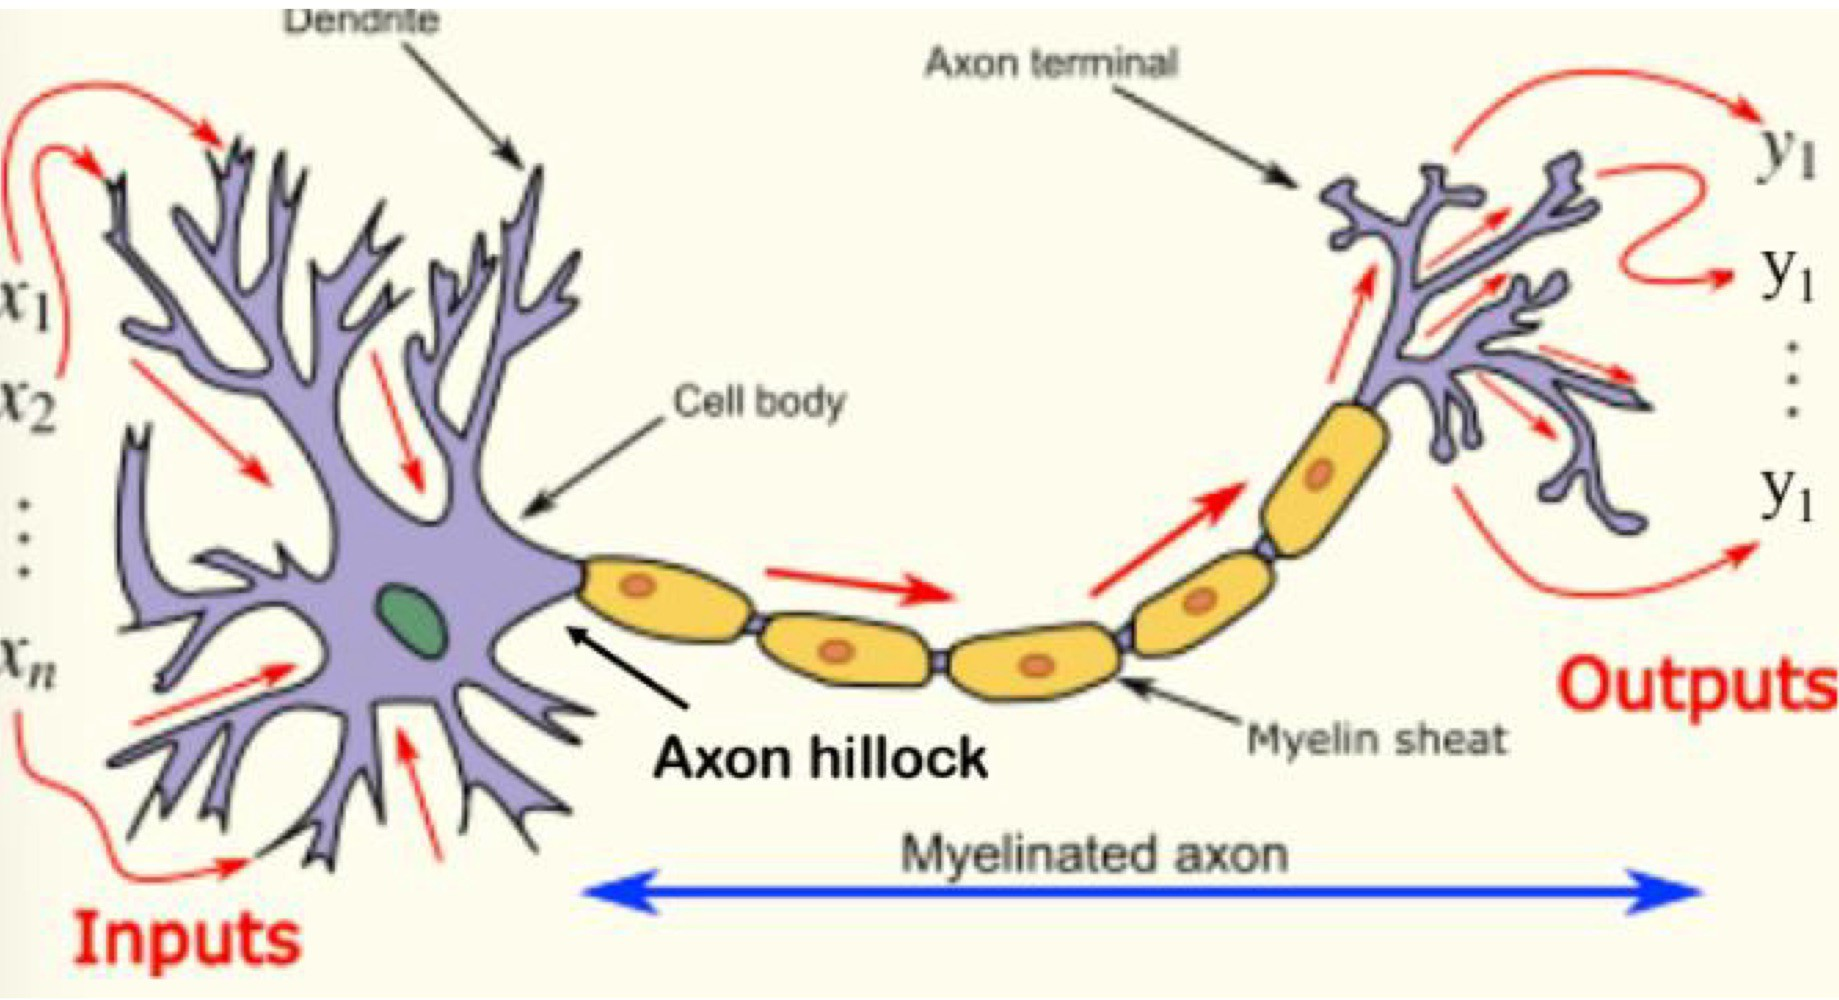
\includegraphics[width=0.80\textwidth]{images/image8.jpeg}
\end{figure}
La struttura delle cellule nervose non è sempre la stessa: ciò che varia è la
forma, mentre le componenti rimangono le medesime.

\subsection{Struttura della membrana neuronale}
Il cuore del funzionamento della cellula nervosa sta nella membrana cellulare: essa è ciò che distingue il neurone dalle altre cellule. Tale membrana svolge varie funzioni: tiene insieme la cellula, le dà una forma e assicura il corretto svolgimento delle funzioni precedentemente elencate. È caratterizzata dalla variazione di tre grandezze elettriche: potenziale di membrana, corrente di membrana e correnti intra extra cellulari.

\begin{figure}[H]
  \centering
  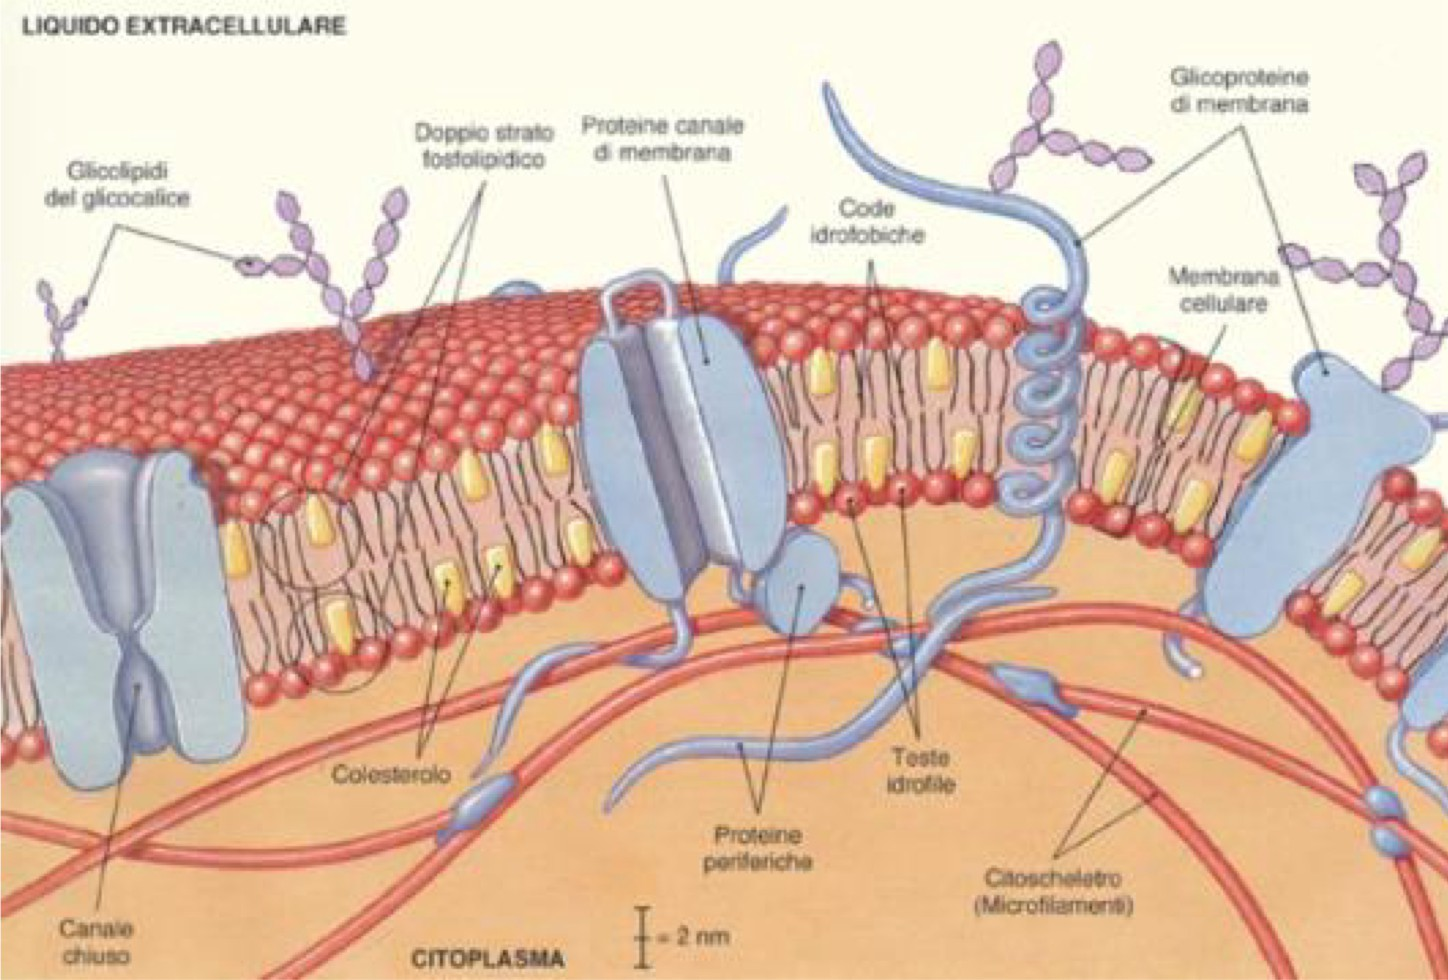
\includegraphics[width=0.80\textwidth]{images/image9.jpeg}
\end{figure}
La membrana è costituita da un doppio strato fosfolipidico, caratterizzato da teste fosforiche e idrofile e da code lipofile (non si collegano con l'acqua ma con i lipidi) e idrofobe, le teste si trovano esternamente mentre le code internamente. La membrana separa la parte interna della cellula (riempita di una soluzione a base acquosa, \textbf{citoplasma} o \textbf{citosol}) dall'esterno (ambiente \textbf{extracellulare}).
Ci sono delle proteine, dette proteine integrali, che attraversano la membrana da parte a parte, permettendo il passaggio controllato di sostanze; esistono delle proteine che si trovano solo sul lato esterno interno e sono dette proteine periferiche.

\subsection{Ioni coinvolti nell'attività neuronale}

I neuroni funzionano grazie al movimento di alcuni ioni (Na$^{+}$, K$^{+}$, Ca$^{2+}$ e Cl$^{-}$) dentro e fuori la cellula. Questi ioni non sono distribuiti in modo uguale: ce ne sono di più fuori o dentro a seconda del tipo (la letteratura ci dice le concentrazioni).
Questa differenza crea due effetti:

\begin{itemize}
  \item una differenza di concentrazione (chimica),
  \item una differenza di carica elettrica (elettrica),
\end{itemize}
Insieme formano la differenza elettrochimica, che è ciò che permette al neurone di trasmettere segnali.


\subsection{Il potenziale di membrana}

Il potenziale di membrana è la differenza di potenziale tra l'interno e l'esterno della cellula, misurata con un voltmetro (elettrodo di riferimento all'esterno, esplorante all'interno). La membrana alterna due condizioni: a riposo, quando è in equilibrio, e attiva, quando varia.
A riposo, il potenziale non è nullo ma rappresenta un ``riposo attivo'', simile a una molla carica, pronto a generare risposta. Tale valore deriva dall'equilibrio tra forze elettriche e chimiche che agiscono sugli ioni (Na$^{+}$, K$^{+}$, Ca$^{2+}$ e Cl$^{-}$).
L'equilibrio elettrochimico è dato da due forze, la differenza di concentrazione e temperatura (la forza chimica) e le forze
elettriche (ioni positivi attratti dal potenziale negativo, ioni negativi dal potenziale positivo).
L'effetto sommato di queste due forze dà origine ad un equilibrio, spiegato dall'equazione di Nernst.

\[
\Delta\mu = \textcolor{red}{RT \ln \frac{[X]_A}{[X]_B}} + \textcolor{blue}{zF(E_A - E_B)}
\]

Il termine chimico (in rosso) scompare se le concentrazioni sono uguali, mentre il termine
elettrico (in blu) dipende da $z$ (valenza, ovvero il numero di carica dello ione: ad esempio
$z=+1$ per Na$^+$ e K$^+$, $z=+2$ per Ca$^{2+}$, $z=-1$ per Cl$^-$) e dalla differenza
di potenziale.

Le due componenti agiscono insieme: se spingono lo ione nella stessa direzione, il movimento è facilitato; se agiscono in direzioni opposte, la direzione dipende dalla loro somma. Quando le due forze si equilibrano, si raggiunge il potenziale di equilibrio, cioè il valore stabile del potenziale di membrana a riposo.


\subsection{Energie in gioco}

Il movimento degli ioni è determinato da due forze principali: il \textbf{gradiente di concentrazione }e il \textbf{potenziale elettrico}.
Gli ioni possiedono energia cinetica dovuta alla temperatura, che li fa muovere casualmente secondo il moto browniano; se c'è una differenza di concentrazione tra due regioni, si crea uno spostamento netto dalla zona più concentrata a quella meno concentrata. Questo meccanismo è proporzionale alla temperatura: più le particelle si muovono velocemente, maggiore sarà la diffusione.
La seconda forza deriva dal potenziale elettrico della membrana. Gli ioni carichi vengono spinti verso l'interno o l'esterno a seconda del segno della loro carica e della polarità del potenziale: ad esempio, un ione positivo sarà attratto verso l'interno se l'interno della cellula è più negativo, mentre un ione negativo sarà respinto verso l'esterno.

In totale, si possono avere quattro combinazioni possibili tra segno della carica e polarità del potenziale, che determinano la direzione dello spostamento. In questo caso l'energia che muove gli ioni è l'energia potenziale elettrica.
Per descrivere questi fenomeni si utilizzano costanti diverse a seconda che si consideri un singolo ione o una mole di ioni: per un singolo ione si usa la costante di Boltzmann, mentre per una mole di ioni si usa la costante universale dei gas, ottenuta moltiplicando la costante di Boltzmann per il numero di Avogadro. L'energia elettrica, invece, dipende dalla valenza dell'ione e dalla differenza di potenziale.
In sintesi, il movimento ionico è il risultato dell'interazione tra energia termica e potenziale elettrico, con direzione e intensità determinate dal gradiente di concentrazione e dal campo elettrico, e con energia fornita rispettivamente dall'energia cinetica e dall'energia potenziale elettrica.


\subsection{Equazione di Nernst}

RECAP: L'equazione di Nernst descrive il potenziale di equilibrio elettrochimico
di un singolo tipo di ione attraverso una membrana. Gli ioni sono soggetti a due
forze principali: la forza chimica e la forza elettrica. Il potenziale di membrana
a cui queste due forze si bilanciano è chiamato \textbf{potenziale di equilibrio},
ed è il valore per cui uno specifico tipo di ione non si sposta più.

Prima di procedere, è utile richiamare i concetti di potenziale di riposo,
depolarizzazione e iperpolarizzazione, che descrivono i possibili stati della
membrana rispetto al suo valore basale di circa $-70$ mV:

\begin{figure}[H]
\centering
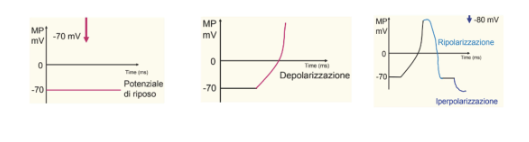
\includegraphics[width=0.85\textwidth]{images/image_stati_membrana.png}
\caption{Da sinistra: potenziale di riposo ($-70$ mV), depolarizzazione
(il potenziale diventa meno negativo) e iperpolarizzazione
(il potenziale diventa più negativo di $-70$ mV).}
\end{figure}

Per trovare il potenziale di equilibrio, si impone $\Delta\mu = 0$
nell'equazione elettrochimica, ricavando la differenza di potenziale
a cui lo ione non si sposta più:

\begin{figure}[H]
\centering
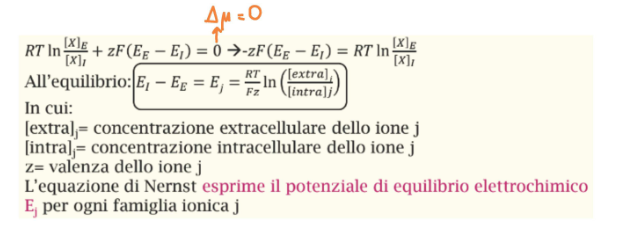
\includegraphics[width=0.80\textwidth]{images/image_nernst_derivazione.png}
\caption{Derivazione dell'equazione di Nernst: ponendo $\Delta\mu = 0$
si ricava il potenziale di equilibrio $E_j$ per ogni famiglia ionica $j$.}
\end{figure}

In generale:
\begin{itemize}
  \item se il potenziale di equilibrio $E_j$ è \textbf{inferiore} al potenziale
    di membrana $V_m$, gli ioni positivi tenderanno a \textbf{uscire} e quelli
    negativi a \textbf{entrare};
  \item se $E_j$ è \textbf{superiore} a $V_m$, gli ioni positivi
    \textbf{entreranno} e quelli negativi \textbf{usciranno}.
\end{itemize}

La tabella seguente riassume il comportamento dei quattro principali ioni
fisiologici, confrontando il loro potenziale di equilibrio con il potenziale
di riposo ($V_m = -70$ mV):

\begin{table}[H]
\centering
\renewcommand{\arraystretch}{1.5}
\begin{tabular}{p{2.5cm} p{2.5cm} p{2.5cm} p{6cm}}
\toprule
\textbf{Ione} & \textbf{$E_j$ (mV)} & \textbf{$V_m = -70$ mV} & \textbf{Cosa succede?} \\
\midrule
K$^+$ & $-90$ mV & $V_m = -70$ mV $\rightarrow$ più positivo di $E_j$ & 
K$^+$ tende a \textbf{uscire} dalla cellula, per portare $V_m$ verso il suo equilibrio più negativo. \\
\midrule
Na$^+$ & $+30$ mV & $V_m = -70$ mV $\rightarrow$ molto più negativo di $E_j$ & 
Na$^+$ tende a \textbf{entrare} nella cellula, per rendere $V_m$ più positivo, avvicinandosi a $+30$ mV. \\
\midrule
Ca$^{2+}$ & $+150$ mV & $V_m = -70$ mV $\rightarrow$ molto più negativo di $E_j$ & 
Ca$^{2+}$ tende a \textbf{entrare} nella cellula, spinto dal gradiente elettrochimico. \\
\midrule
Cl$^-$ & $-70$ mV & $V_m \approx E_j$ $\rightarrow$ quasi in equilibrio & 
Cl$^-$ è \textbf{quasi in equilibrio}: ha poco movimento netto. Se $V_m$ diventasse più negativo, Cl$^-$ tenderebbe a entrare; se più positivo, uscirebbe. \\
\bottomrule
\end{tabular}
\caption{Potenziali di equilibrio e comportamento atteso per i principali ioni
fisiologici a $V_m = -70$ mV.}
\end{table}

\subsection{Meccanismi di trasporto di membrana}

Gli spostamenti che avvengono seguendo il gradiente elettrochimico (visti ora) prendono il nome di \textbf{trasporto passivo}, in quanto lo spostamento avviene esclusivamente mediante l'energia (cinetica potenziale) fornita dagli ioni stessi.

Tuttavia esiste un altro tipo di trasporto detto \textbf{trasporto attivo}, non utilizza il gradiente elettrochimico (gli ioni si spostano contro gradiente) ma le \textbf{pompe ioniche}. L'energia usata questa volta è fornita dalla cellula ed è l'\textbf{ATP}.

Esistono diverse pompe ioniche, la più importante è la \textbf{pompa sodio-potassio}.
\begin{figure}[H]
\centering
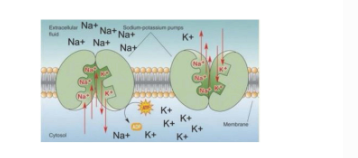
\includegraphics[width=0.80\textwidth]{images/sodio-potassio.png}
\end{figure}
La pompa sodio-potassio cambia la sua conformazione per esporre alternativamente i siti di legame verso l'interno o l'esterno della cellula. Durante il ciclo, trasporta 3 ioni sodio dall'interno verso l'esterno e 2 ioni potassio dall'esterno verso l'interno, consumando 1 molecola di ATP per ogni ciclo. Questo meccanismo non simmetrico permette di mantenere e ripristinare l'equilibrio ionico della cellula.

\subsection{Cause del potenziale di riposo}

Le quattro principali famiglie ioniche (Na$^{+}$, K$^{+}$, Cl$^{-}$, Ca$^{2+}$) vengono continuamente spostate attraverso la membrana dai tre meccanismi visti: diffusione, forze elettriche e pompe ioniche. Nonostante questo movimento costante, il potenziale di membrana rimane stabile nel tempo, perché la risultante di tutti gli spostamenti è bilanciata.
Questo stato di equilibrio dinamico prende il nome di \textbf{potenziale di riposo}, che nei neuroni è di circa -70 mV, con l'interno della cellula più negativo rispetto all'esterno, quindi la membrana è polarizzata.
Quando si verifica una perturbazione, flussi di ioni positivi attraversano la membrana, riducendo la sua polarizzazione: questo fenomeno si chiama \textbf{depolarizzazione}. Gli ioni che provocano questo effetto sono detti \textit{ioni depolarizzanti}, e le correnti generate si chiamano \textit{correnti depolarizzanti}. Successivamente, la membrana può tornare al potenziale di riposo attraverso la \textbf{ripolarizzazione}, dovuta a \textit{ioni e correnti ripolarizzanti}. Se la membrana diventa ancora più negativa del valore di riposo, si verifica l'\textbf{iperpolarizzazione}, cioè un aumento della polarizzazione.


\subsection{Diffusione facilitata: i canali ionici}

La diffusione facilitata avviene tramite \textbf{canali ionici}, tali proteine che
permettono il passaggio selettivo di specifici ioni attraverso la membrana, senza
consumo di energia (\textit{passaggio selettivo di ioni in modo passivo}), poiché
agiscono secondo gradiente di concentrazione.
Ogni canale è \textbf{selettivo}: ad esempio, un canale per il sodio non permette
il passaggio del potassio e viceversa.
I canali possono essere sempre aperti oppure dotati di un ``cancello'' che ne regola
l'apertura e la chiusura. L'apertura di questi canali può dipendere da diversi fattori:
\begin{itemize}
  \item agenti chimici (che si legano al canale direttamente o indirettamente, come
    nei recettori sinaptici) $\rightarrow$ canali chimico-dipendenti;
  \item variazioni del potenziale di membrana $\rightarrow$ canali voltaggio-dipendenti;
  \item stimoli fisici come luce, temperatura o pressione $\rightarrow$ canali attivati
    da stimoli fisici.
\end{itemize}

\textbf{Canale Na\textsuperscript{+} voltaggio-dipendente}
Il canale del sodio è una proteina di membrana che può assumere tre configurazioni: chiuso, aperto e inattivo. Nello stato di chiusura, il canale non permette il passaggio di ioni ma può aprirsi; nello stato di apertura, cambia forma e lascia passare gli ioni sodio; nello stato di inattivazione, il passaggio degli ioni è nuovamente impedito, ma il canale non può riaprirsi direttamente, deve prima tornare allo stato di chiusura.

\begin{wrapfigure}{H}{0.45\textwidth}
  \centering
  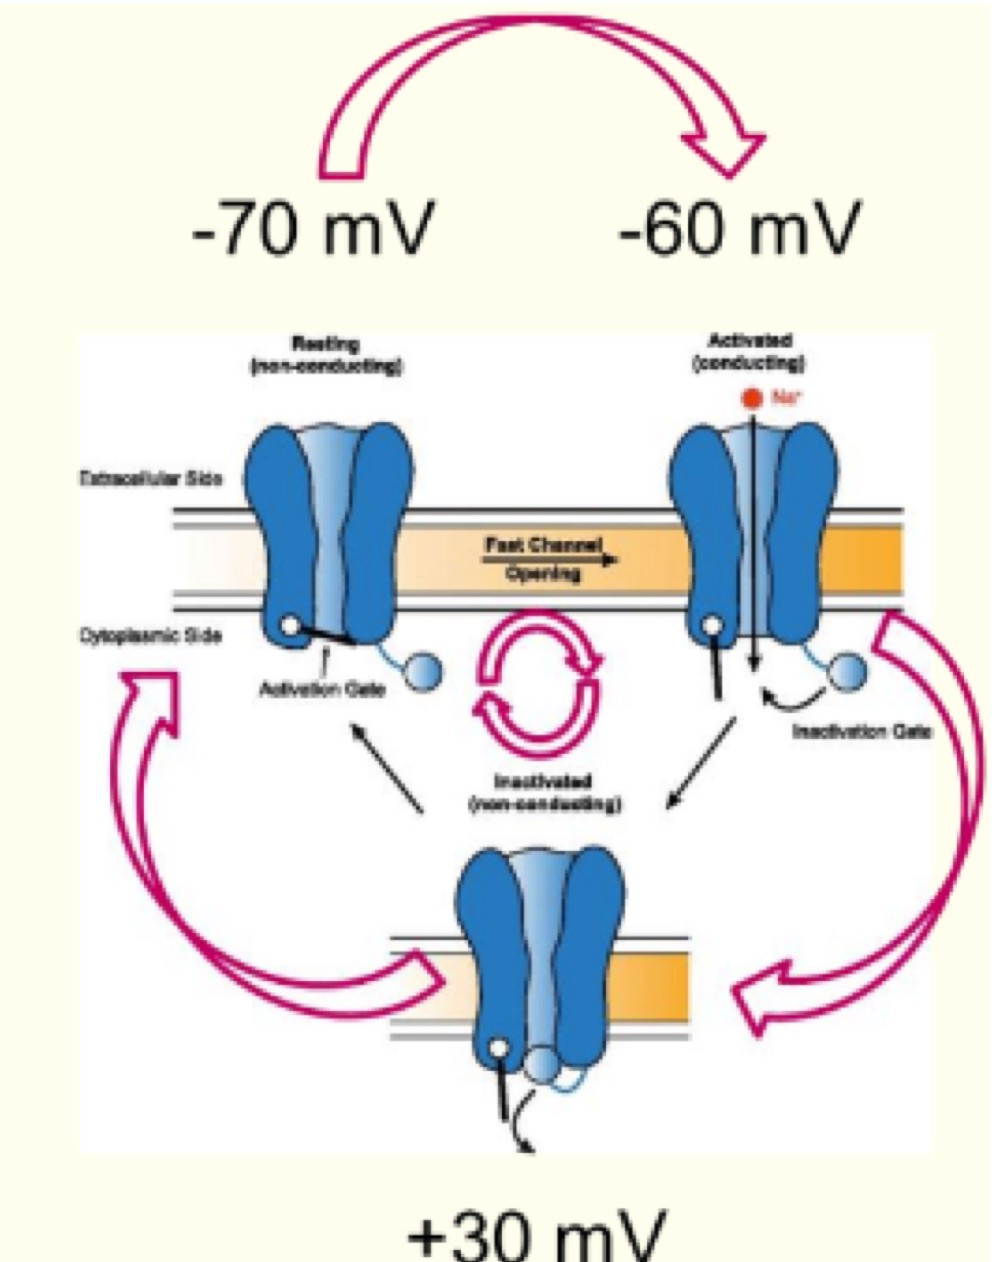
\includegraphics[width=0.30\textwidth]{images/image13.jpeg}
\end{wrapfigure}

Il passaggio tra questi stati dipende dal potenziale di membrana, che determina soglie specifiche di attivazione e inattivazione:

\begin{itemize}
  \item A --70 mV (potenziale di riposo), il canale è chiuso;
  \item Se il potenziale si depolarizza e raggiunge circa --60 mV, il canale si apre, permettendo l'ingresso di ioni sodio dall'esterno verso l'interno, secondo gradiente elettrochimico;
  \item L'ingresso di sodio aumenta la depolarizzazione fino a circa +30 mV, momento in cui il canale si inattiva e il flusso ionico si interrompe.
\end{itemize}

\begin{wrapfigure}{H}{0.45\textwidth}
  \centering
  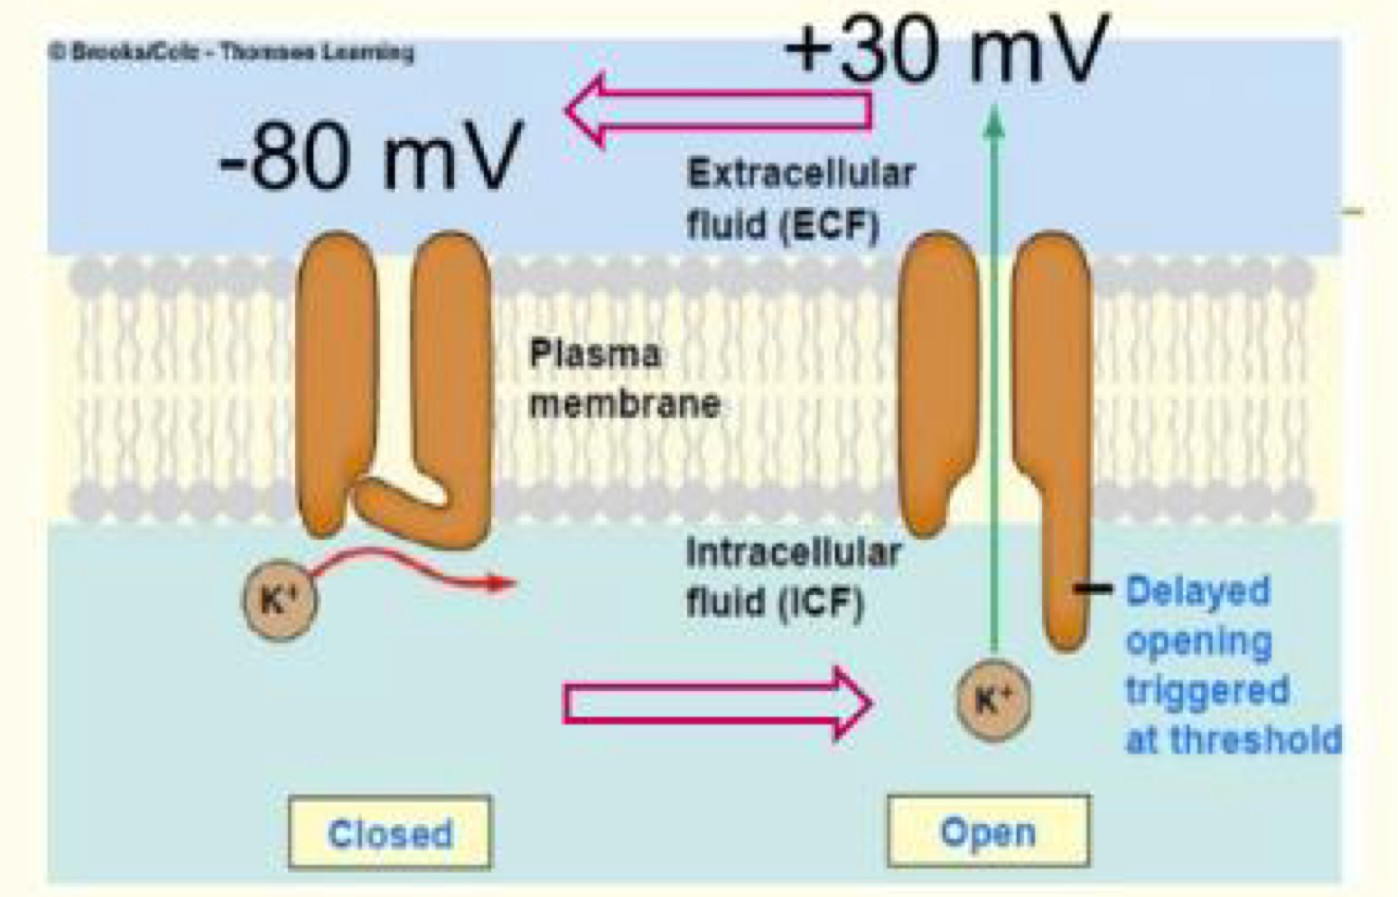
\includegraphics[width=0.40\textwidth]{images/image14.jpeg}
\end{wrapfigure}
Quando la membrana si ripolarizza (torna negativa), il canale non si riapre subito, ma passa dallo stato inattivo a quello chiuso a --70 mV, pronto a riattivarsi in seguito. Lo stato di inattività ha la funzione di impedire una riapertura troppo precoce del canale, garantendo che la sequenza di apertura e chiusura avvenga in modo ordinato e controllato durante il potenziale d'azione.
\textbf{Canale K+ voltaggio-dipendente}
Il canale del potassio (K$^{+}$) a voltaggio-dipendente è un canale a cancello elettricamente controllato, che cambia configurazione in base al potenziale di membrana. Può trovarsi solo in due stati: \textbf{aperto }o \textbf{chiuso}, con due soglie precise: +30 mV per l'apertura e --80 mV per la chiusura. A riposo (--70 mV) il canale è chiuso. Quando avviene una depolarizzazione, il canale rimane chiuso fino al raggiungimento di +30 mV, valore in cui il canale del sodio si inattiva e quello del potassio si apre, permettendo il passaggio degli ioni K$^{+}$. Il canale del potassio quindi agisce in senso opposto a quello del sodio, contribuendo al ritorno del potenziale a valori negativi.

\begin{figure}[H]
  \centering
  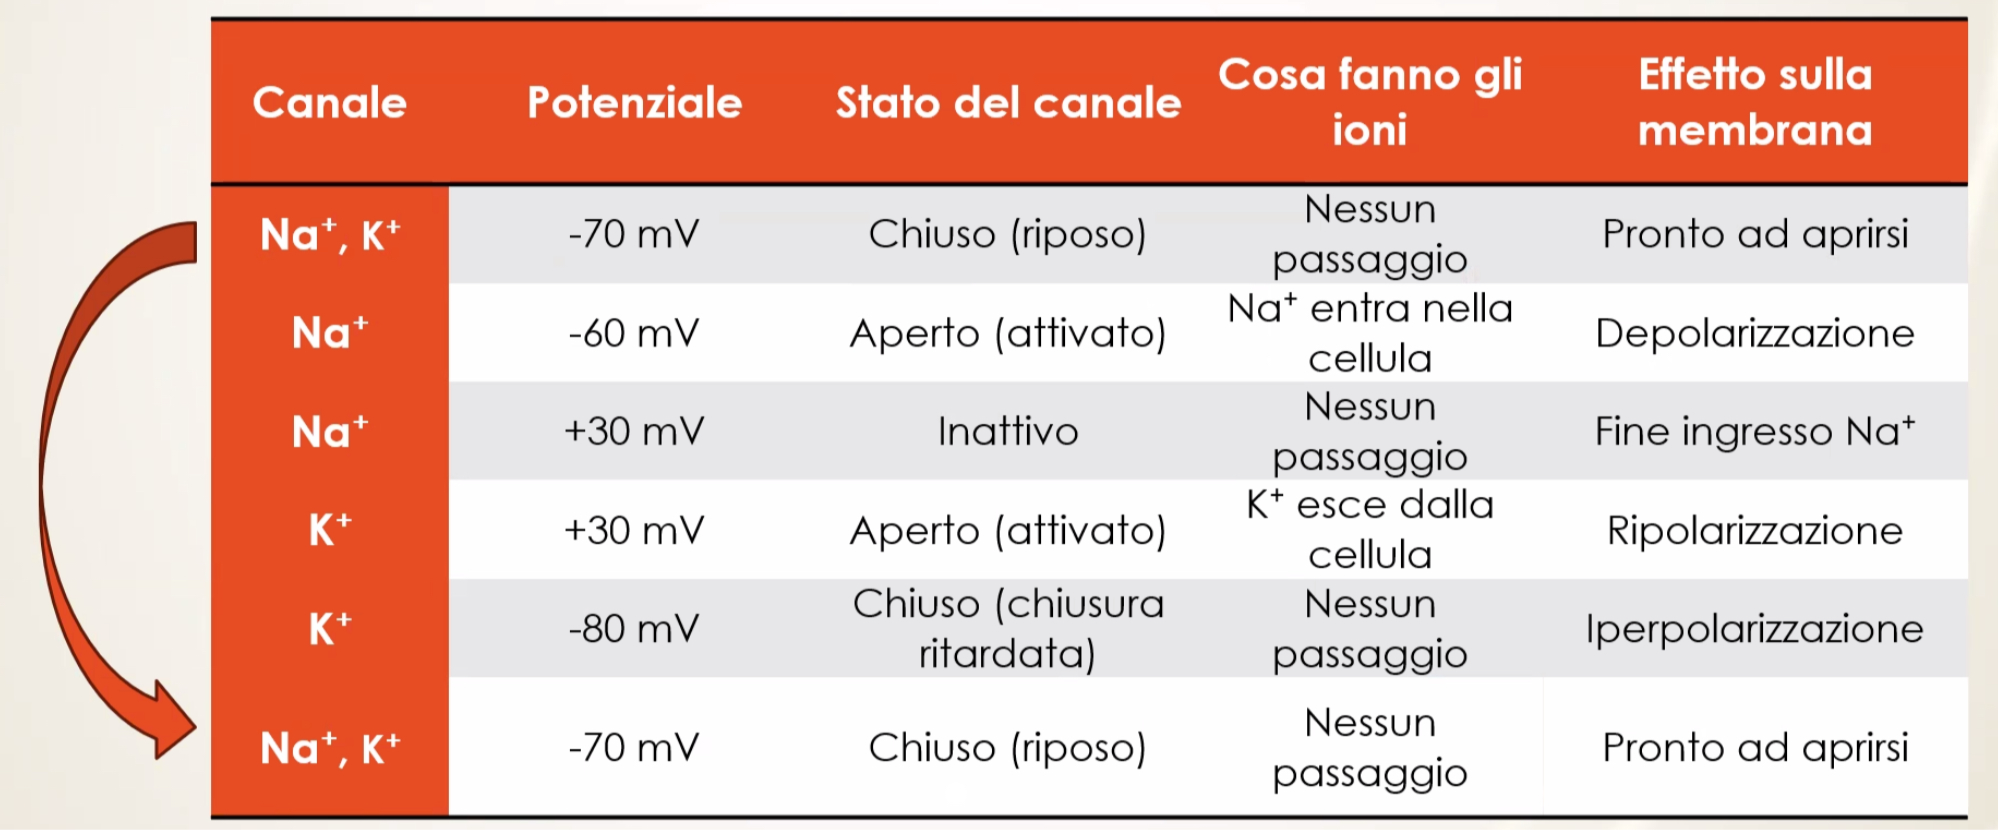
\includegraphics[width=0.65\textwidth]{images/image15.png}
\end{figure}

La soglia di chiusura è --80 mV, inferiore al potenziale di riposo (--70 mV), perciò è necessaria un'iperpolarizzazione per richiudere il canale. Poiché il potenziale di equilibrio del K$^{+}$ è --90 mV, gli ioni potassio continuano a uscire anche oltre i --80 mV, spingendo la membrana verso l'iperpolarizzazione e favorendo la chiusura del canale.
\textbf{1b. Generazione e propagazione del potenziale d'azione, potenziali graduati}

\subsection{Il potenziale d'azione}

Il potenziale d'azione è una variazione del potenziale di membrana (da qui ``potenziale'') osservabile in punti specifici della cellula, che permette alla cellula di inviare segnali ad altre cellule, entrando così ``in azione'' (da qui ``d'azione'').
Non tutte le cellule lo generano: solo le \textbf{cellule eccitabili }(nervose, muscolari striate e cardiache).
Ha una forma sempre identica, con ampiezza, durata e andamento costanti, per cui l'informazione non dipende da queste caratteristiche.
Funziona secondo il principio del ``tutto o nulla'': o non avviene, oppure, se si genera, è sempre uguale, come un segnale binario (0 o 1).
Si verifica quando la membrana si depolarizza fino a circa -60 mV, indicando che è regolato da un meccanismo a soglia.

\subsection{Generazione del potenziale d'azione}

In figura è rappresentato l'andamento del potenziale d'azione. Sull'asse delle ascisse si ha il tempo in ms, mentre sull'asse delle ordinate si ha il potenziale di membrana, espresso in mV.
\begin{figure}[H]
  \centering
  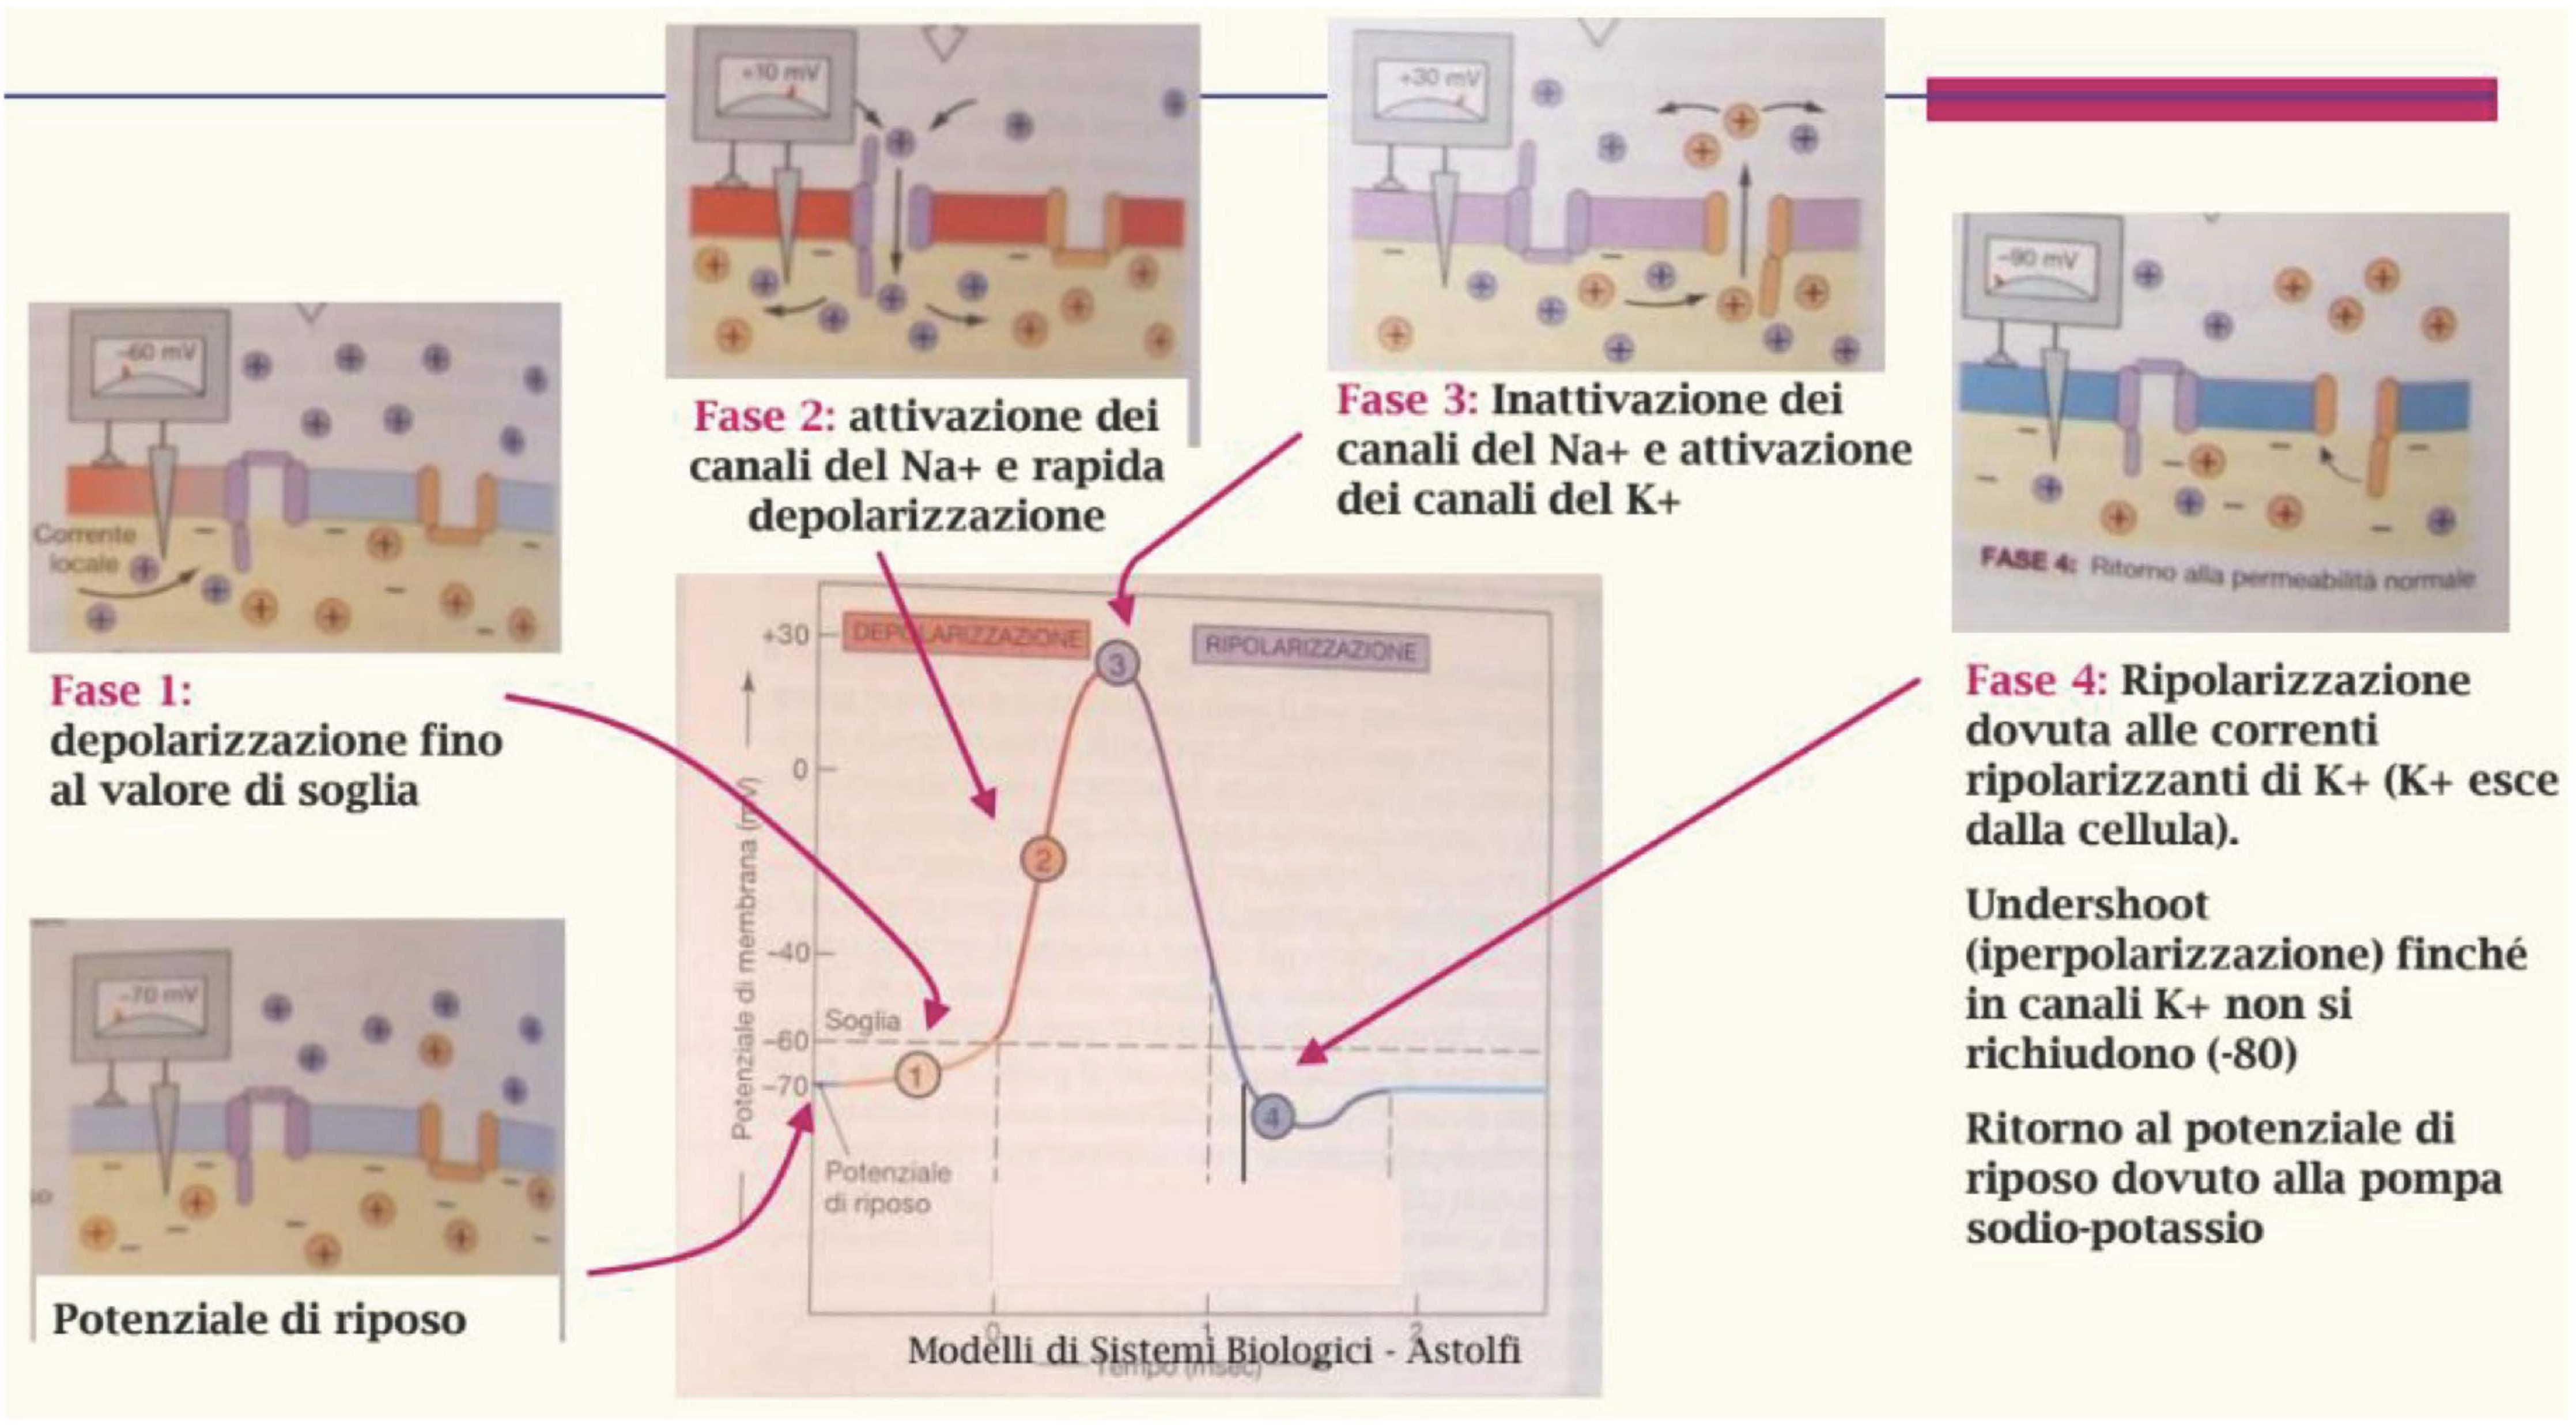
\includegraphics[width=0.80\textwidth]{images/image17.jpeg}
\end{figure}
La generazione del potenziale d'azione segue un andamento preciso nel tempo:

\begin{itemize}
  \item \textbf{Riposo}: la membrana è a -70 mV, con canali di sodio e potassio chiusi. Piccole variazioni intorno al potenziale di riposo possono avvenire, ma il meccanismo importante parte solo quando si raggiunge la soglia di -60 mV.
  \item \textbf{fase 1- Soglia di attivazione }(-60 mV): se la depolarizzazione raggiunge questa soglia, si apre il canale del sodio.
  \item \textbf{fase 2 - Depolarizzazione rapida}: gli ioni sodio entrano nella cellula, causando un rapido aumento del potenziale fino a circa +30 mV. Il canale del sodio si inattiva a questo punto, interrompendo il flusso.
  \item \textbf{fase 3 - Ripolarizzazione}: si aprono i canali del potassio; il potassio esce dalla cellula, riportando la membrana verso il potenziale di riposo (-70 mV). I canali del potassio si chiudono a -80 mV, causando un'iperpolarizzazione temporanea.
  \item \textbf{fase 4 - Ripristino dell'equilibrio}: le pompe sodio-potassio riportano gli ioni nelle loro posizioni iniziali, ripristinando completamente il potenziale di membrana.
\end{itemize}
Indipendentemente dal percorso iniziale, una volta raggiunta la soglia di -60 mV, il meccanismo è sempre lo stesso: apertura e chiusura dei canali e delle pompe sono costanti, così come il numero di ioni coinvolti.


\subsection{Refrattarietà assoluta}

Quando la membrana parte dal potenziale di riposo (-70 mV) e raggiunge la soglia, si apre il canale del sodio, che permette agli ioni sodio di entrare e avviare il potenziale d'azione. Poco dopo, però, questo canale diventa inattivo:

\begin{itemize}
  \item Quando è aperto, il sodio può passare normalmente;
  \item Quando è inattivo, il canale non può più aprirsi, nemmeno se lo stimolo sulla
  \item membrana diventa molto forte.
\end{itemize}
Questo significa che durante questo intervallo (viola nell'immagine) non può essere generato nessun nuovo potenziale d'azione.
Questo periodo prende il nome di \textbf{refrattarietà assoluta}: la membrana è completamente refrattaria, cioè oppone resistenza totale alla generazione di un nuovo potenziale d'azione.
In pratica, la refrattarietà assoluta dipende solo dai canali del sodio e non ammette eccezioni: finché i canali sono inattivi, il potenziale d'azione non può ricominciare. Termina quando i canali Na+ si chiudono (-70mV).


\subsection{Refrattarietà relativa}

La refrattarietà relativa inizia subito dopo la refrattarietà assoluta, quando i canali del sodio, che prima erano inattivi, si chiudono di nuovo intorno a -70 mV.
In questo momento la membrana non è ancora al potenziale di riposo perché i canali del potassio sono ancora aperti, causando una iperpolarizzazione.
I canali del sodio sono però pronti a riaprirsi, quindi è possibile generare un nuovo potenziale d'azione, ma serve uno stimolo più forte del normale, superiore ai 10 mV necessari a raggiungere la soglia di -60 mV.
Questo periodo prende il nome di \textbf{refrattarietà relativa}: la membrana non
impedisce completamente un nuovo potenziale d'azione, ma rende la sua generazione più difficile.

A differenza della refrattarietà assoluta, che dipende dai canali del sodio, quella relativa dipende dai canali del potassio ancora aperti. Termina quando i canali K+ si chiudono (-80mV).


\subsection{Sequenze di potenziale d'azione}

La cellula, in tempi brevissimi (1-2 ms), valuta continuamente se generare nuovi potenziali d'azione. La linea azzurra indica il potenziale di riposo, mentre la linea rossa rappresenta la soglia di attivazione.
Non tutte le variazioni del potenziale di membrana raggiungono la soglia: quelle più piccole, che non provocano un potenziale d'azione, si chiamano potenziali graduati. Questi sono meno ampi e più lunghi dei potenziali d'azione veri e propri.

\begin{figure}[H]
  \centering
  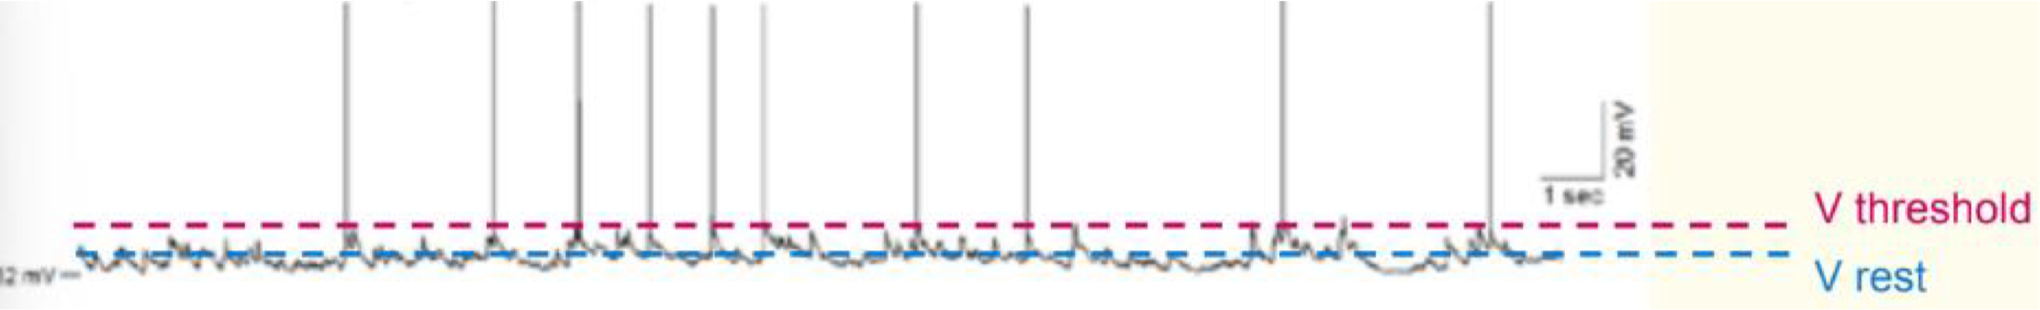
\includegraphics[width=0.80\textwidth]{images/image20.png}
\end{figure}

I potenziali d'azione, invece, si generano solo quando la perturbazione della membrana supera la soglia. Essendo tutti identici per ampiezza, forma e durata, l'informazione non sta nel singolo potenziale, ma nella sequenza con cui essi si susseguono. In altre parole, ciò che conta è quando avviene ogni potenziale d'azione e quanto spazio temporale c'è tra due segnali consecutivi, perché da questo dipende la risposta della cellula.
Brevissima durata, ampiezza elevata: simile a uno \textbf{spike }(delta di Dirac).
L'informazione non è contenuta nella forma.

\section{Propagazione del potenziale d’azione}

Il potenziale d’azione può essere registrato in diversi distretti della cellula. I canali ionici voltaggio-dipendenti, infatti, sono presenti sul soma, sui dendriti e, in concentrazione particolarmente elevata, sul cono d’emergenza dell’assone e lungo l’assone stesso. È proprio l’elevata densità di canali del sodio a fare del cono d’emergenza il sito in cui, con maggiore probabilità, il potenziale d’azione viene innescato.
Le informazioni raccolte dai dendriti vengono integrate dal neurone e convertite in una variazione del potenziale di membrana che si propaga fino al cono d’emergenza. Se tale perturbazione supera il valore soglia, in questa regione si genera il potenziale d’azione, che viene successivamente propagato lungo l’assone.
La propagazione può avvenire secondo due modalità, che dipendono dalla struttura dell’assone:
\begin{itemize}
    \item \textbf{continua}, nelle fibre amieliniche;
    \item \textbf{saltatoria}, nelle fibre mieliniche.
\end{itemize}

\begin{figure}[H]
    \centering
    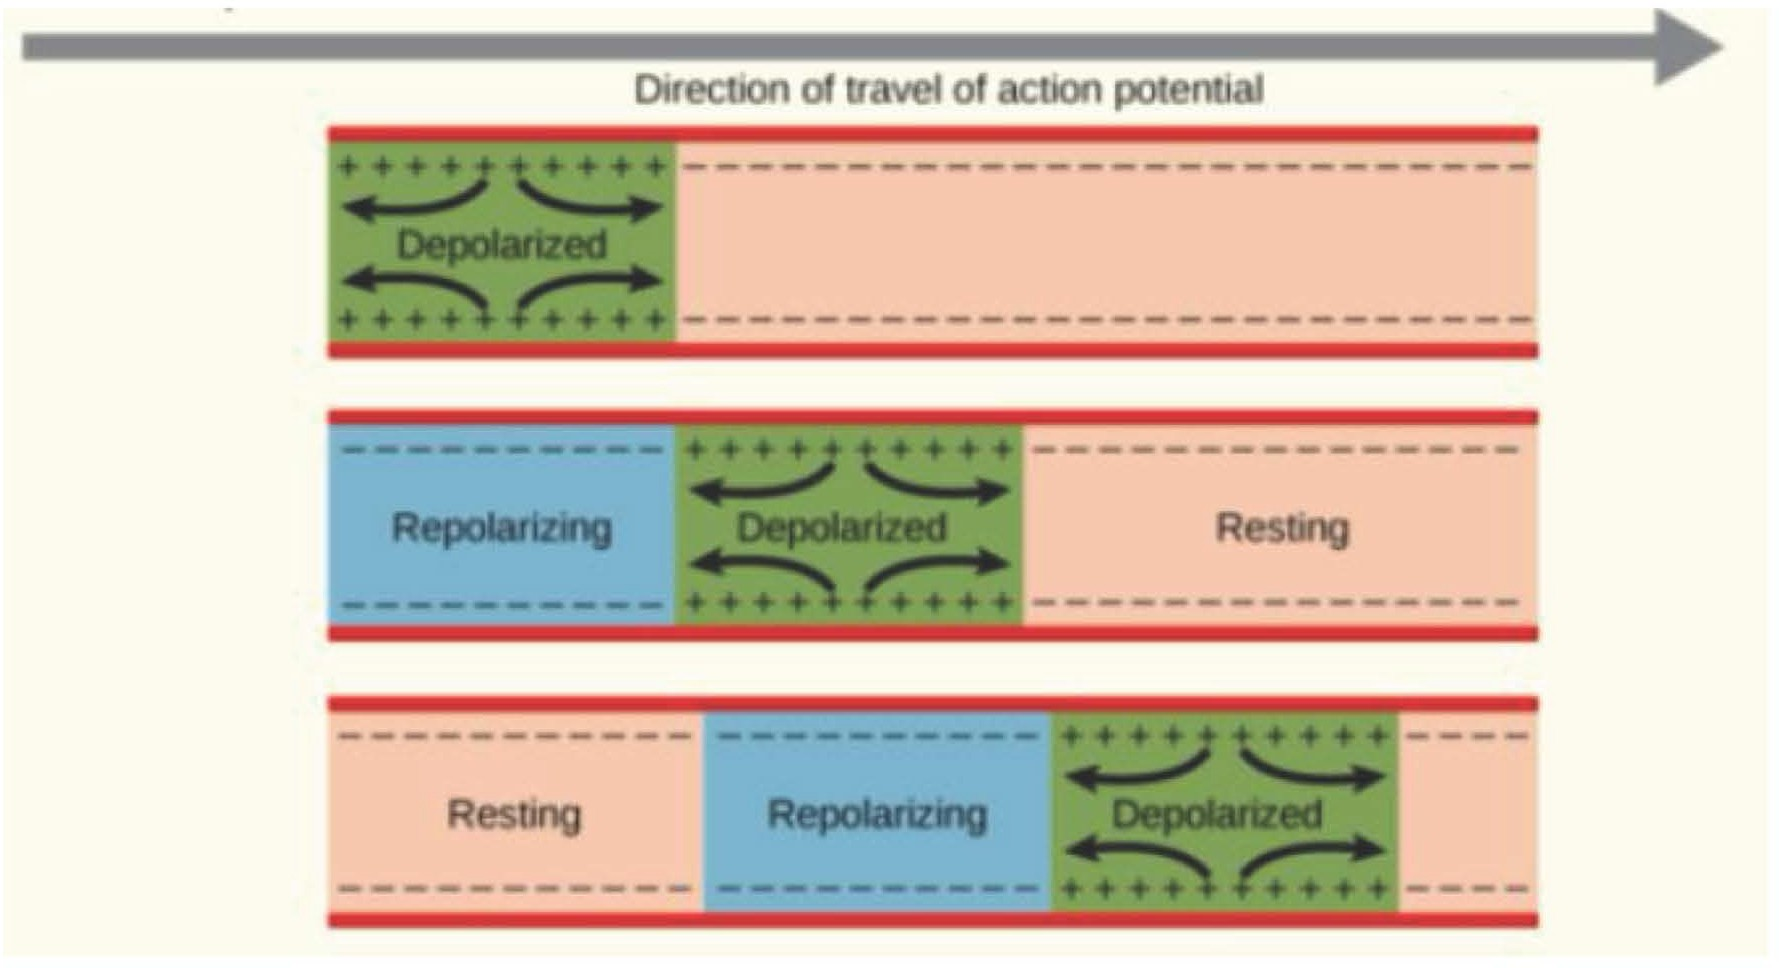
\includegraphics[width=0.80\textwidth]{images/image21.jpeg}
    \caption{Propagazione continua del potenziale d’azione.}
\end{figure}

\subsection{Propagazione continua}

Quando in un punto della membrana assonale si scatena un potenziale d’azione, si verifica localmente un’inversione della polarità: l’interno diventa positivo rispetto all’esterno. Al contrario, le regioni adiacenti si trovano ancora al potenziale di riposo, con cariche negative sul versante intracellulare e positive su quello extracellulare. Questa differenza genera correnti ioniche locali: le cariche positive diffondono all’interno dell’assone verso le zone a potenziale minore, mentre all’esterno si muovono in direzione opposta. Tali flussi prendono il nome di \textbf{correnti locali}.
Questo meccanismo è detto \textbf{propagazione passiva} (da non confondere con il trasporto passivo di membrana). Non riguarda unicamente il potenziale d’azione, ma qualsiasi perturbazione del potenziale di membrana. Le sue proprietà fondamentali sono:
\begin{itemize}
    \item è \textbf{adirezionale}, poiché le cariche si spostano in tutte le direzioni seguendo il gradiente elettrochimico;
    \item è \textbf{dipendente dalla distanza}, attenuandosi progressivamente allontanandosi dal punto d’origine;
    \item si \textbf{estingue rapidamente} se non viene rigenerata.
\end{itemize}

Nel caso del potenziale d’azione, la perturbazione iniziale è molto ampia (circa 100 mV). La depolarizzazione che ne deriva, propagandosi passivamente alle zone adiacenti, mantiene un’intensità ancora considerevole (sempre inferiore a 100 mV, ma comunque superiore ai 10 mV necessari per attivare i canali voltaggio-dipendenti). In questo modo, la propagazione passiva è in grado di depolarizzare la membrana circostante fino alla soglia.
Il potenziale d’azione si propaga pertanto rigenerandosi punto per punto lungo l’assone: la perturbazione si trasmette passivamente al tratto adiacente, vi innesca un nuovo potenziale d’azione, che a sua volta si propaga passivamente al segmento successivo, e così via. Questo processo prende il nome di \textbf{conduzione attiva}. Esso richiede un notevole dispendio energetico ed è intrinsecamente più complesso e lento della semplice propagazione passiva.
La propagazione passiva, essendo basata sulla diffusione, è per sua natura adirezionale. Tuttavia, il potenziale d’azione viaggia nell’assone in direzione centrifuga, ovvero dal corpo cellulare verso le terminazioni sinaptiche. L’unidirezionalità è garantita dal \textbf{periodo refrattario assoluto}: la regione di membrana che ha appena generato un potenziale d’azione si trova con i canali del sodio inattivati e non può essere rieccitata. Il potenziale può così propagarsi soltanto verso il tratto di membrana ancora a riposo, situato anteriormente.
La propagazione continua è un meccanismo relativamente lento, con una velocità media di circa 1 m/s. Le vie dolorose, ad esempio, sono vie a conduzione lenta che utilizzano proprio questa modalità di propagazione.

\subsection{La propagazione saltatoria}

La propagazione saltatoria si basa su una diversa struttura dell’assone. Rispetto all’assone “nudo” della conduzione continua, qui intervengono le cellule di Schwann, che avvolgono l’assone in più strati formando una guaina mielinica, simile a un nastro isolante. Questa guaina isola l’interno dall’esterno e impedisce il passaggio di sostanze.
La mielina non ricopre tutta la lunghezza dell’assone: esistono delle interruzioni chiamate nodi di Ranvier, dove la membrana è esposta e sono presenti canali del sodio e del potassio voltaggio-dipendenti.
La propagazione procede così: si genera la perturbazione, si produce una forte depolarizzazione, segue una breve e rapida propagazione passiva, e poi si genera un potenziale d’azione, che è sempre uguale. L’assone rivestito si chiama assone mielinizzato; gruppi di assoni mielinizzati costituiscono le fibre nervose. Nel segmento mielinizzato la depolarizzazione si propaga passivamente, ma non può generare nuovi potenziali d’azione perché non c’è comunicazione tra interno ed esterno (la guaina isola). Quindi in quel tratto non possono attivarsi i canali: le correnti scorrono passivamente fino al nodo successivo.
Al nodo successivo, se la distanza tra i nodi è adeguata, la perturbazione, pur attenuandosi lungo il tratto mielinizzato, arriva ancora con un’ampiezza di almeno 10 mV nella direzione della depolarizzazione, sufficiente a generare un nuovo potenziale d’azione. La distanza tra i nodi è ottimizzata per questo. I vantaggi sono:
\begin{itemize}
    \item generazione di potenziali solo nei nodi e non lungo tutto l’assone;
    \item maggiore efficienza;
    \item velocità molto elevata: circa 120 m/s.
\end{itemize}
Le vie motorie sono mielinizzate, mentre quelle dolorifiche non lo sono.
Si parla di conduzione saltatoria perché il potenziale d’azione sembra comparire, sparire e poi ricomparire ai nodi, come se “saltasse” da un nodo all’altro.

\section{La trasmissione sinaptica e l’integrazione dell’informazione}

La trasmissione dell’informazione avviene sempre tra due cellule: una cellula \textbf{inviante} (che può essere un neurone o uno stimolo esterno) e una cellula \textbf{ricevente}. L’informazione viene trasmessa sotto forma di \textbf{potenziale d’azione}, ossia una depolarizzazione intensa del potenziale di membrana, che viaggia lungo l’assone fino a raggiungere altre cellule. Questo processo prende il nome di \textbf{trasmissione sinaptica} e avviene attraverso le sinapsi, che rappresentano le strutture fisiche responsabili del passaggio dell’informazione da una cellula all’altra.
Le cellule che ricevono informazioni possiedono dendriti, siti specifici organizzati in una struttura ramificata chiamata albero dendritico. La forma dell’albero dendritico può variare: esistono cellule con strutture diverse, ma tutte condividono la struttura base composta da soma e ramificazioni con forma e distribuzione differenti. Le informazioni inviate dalla cellula si presentano come un unico segnale che cambia nel tempo, e possono essere molteplici e di origine diversa. Esso inoltre è un segnale elettrico, cioè una variazione di una grandezza elettrica, che viaggia tra le cellule creando una connessione elettrica per trasferire l’informazione. L’informazione ha la forma di un segnale elettrico, cioè una variazione di una grandezza elettrica che viaggia da una cellula all’altra creando una connessione utile al trasferimento. Questo fenomeno in natura prende il nome di sinapsi elettrica, anche se non è il meccanismo più comune. In ogni sinapsi ci sono due cellule: la pre-sinaptica, che invia l’informazione, e la post-sinaptica, che la riceve. I ruoli non sono interscambiabili. I principali vantaggi della sinapsi elettrica sono la velocità elevata e la sincronizzazione tra cellule.
La cellula pre-sinaptica invia il segnale sotto forma di potenziale d’azione (impulso nervoso). In realtà arriva una sequenza di potenziali d’azione, ma consideriamo un singolo impulso: esso percorre l’assone fino al bottone sinaptico, dove incontra la cellula post-sinaptica. Quest’ultima riceve l’informazione tramite il proprio albero dendritico. Nelle sinapsi elettriche le membrane pre e post-sinaptiche sono collegate da gap junctions, proteine che ancorano le due membrane e mettono in continuità i liquidi intracellulari. I loro pori, sempre aperti, permettono il passaggio libero degli ioni tra le cellule. Quando arriva l’impulso nervoso, si verifica una depolarizzazione: le cariche positive passano alla cellula post-sinaptica, che si depolarizza a sua volta. In questo modo il segnale viene trasmesso mantenendo la sua natura elettrica.

Questo meccanismo, però, ha un limite: poiché il segnale è sempre una depolarizzazione, l’effetto sulla membrana post-sinaptica è sempre lo stesso, positivo. Non può mai cambiare segno. Per questo motivo la sinapsi elettrica, pur essendo semplice, veloce e sincronizzata, risulta poco comune.
La sinapsi chimica è un meccanismo molto più diffuso e complesso, ma con enormi vantaggi. In questa sinapsi le due cellule \textbf{non} si toccano, non esiste una continuità fisica, ma uno spazio detto \textbf{fessura sinaptica}. L’informazione elettrica che arriva sulla cellula pre-sinaptica cambia natura: diventa un segnale chimico per attraversare la fessura e raggiungere la cellula post-sinaptica. Il messaggero è quindi di tipo chimico, e il segnale passa da elettrico a chimico, per poi tornare di nuovo elettrico. La trasformazione è mediata dai neurotrasmettitori.

\begin{figure}[H]
    \centering
    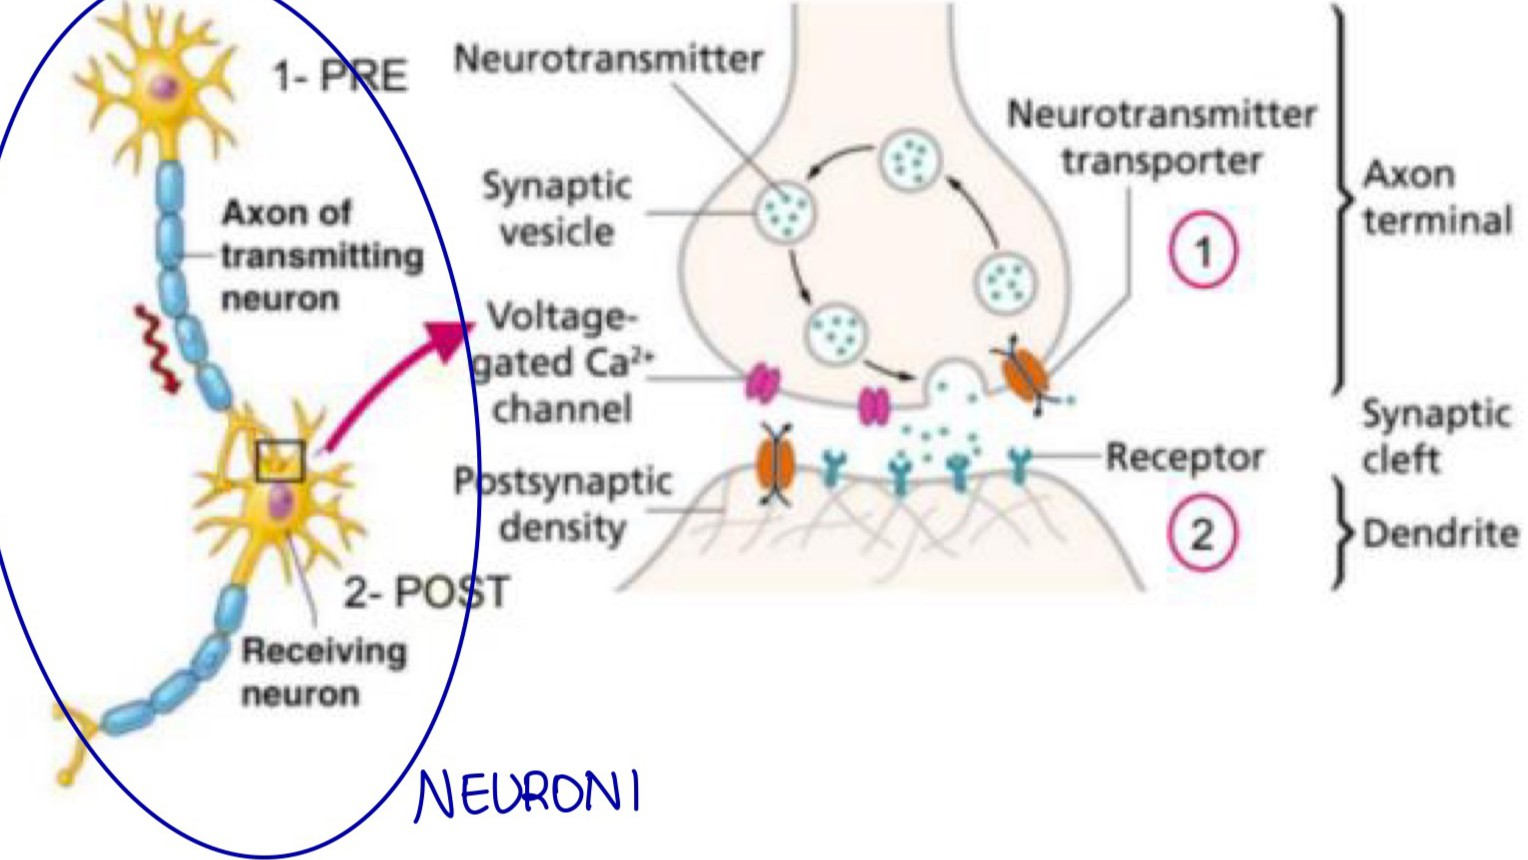
\includegraphics[width=0.80\textwidth]{images/image24.jpeg}
\end{figure}

Nell’immagine si osservano due neuroni che fanno sinapsi, l’arrivo del potenziale d’azione lungo l’assone mielinizzato e l’ingrandimento della fessura sinaptica tra il bottone sinaptico del neurone pre-sinaptico e l’albero dendritico del neurone post-sinaptico. Perché avvenga una sinapsi chimica sono necessarie strutture specifiche. Nella cellula pre-sinaptica, lungo la membrana, ci sono canali voltaggio-dipendenti per lo ione calcio. Quando arriva il potenziale d’azione, i canali si aprono: il calcio, presente soprattutto all’esterno, entra nella cellula secondo il gradiente elettrochimico. Questo ingresso attiva il meccanismo di rilascio del neurotrasmettitore tramite esocitosi. Il processo è unidirezionale: il neurone pre-sinaptico trasmette, quello post-sinaptico riceve.
I neurotrasmettitori, contenuti in vescicole nel bottone sinaptico, vengono liberati con l’esocitosi: le vescicole si fondono con la membrana e rilasciano il contenuto nella fessura sinaptica. A questo punto interviene la cellula post-sinaptica, dotata di strutture per ricevere il segnale:
\begin{itemize}
    \item \textbf{canali a cancello chimico}, che si aprono solo in presenza del neurotrasmettitore;
    \item \textbf{recettori}, proteine specifiche capaci di legarsi con una particolare molecola di neurotrasmettitore.
\end{itemize}
Se il neurotrasmettitore non è presente nella fessura, i canali rimangono chiusi e la membrana resta a riposo. Ciò può avvenire se il potenziale d’azione non è arrivato, se non c’è abbastanza neurotrasmettitore o se manca il calcio necessario al rilascio. Quando invece il potenziale d’azione raggiunge la cellula pre-sinaptica e avviene il rilascio, il neurotrasmettitore si lega ai recettori e apre i canali ionici. Questo può avvenire in due modalità: \textbf{ionotropica} o \textbf{metabotropica}. Il canale permette il passaggio di ioni secondo gradiente, generando correnti di membrana, dette correnti sinaptiche, che modificano il potenziale di membrana producendo i potenziali post-sinaptici. Il meccanismo non è ciclico e si interrompe in tre modi:
\begin{itemize}
    \item \textbf{degradazione enzimatica del neurotrasmettitore} e successivo smaltimento;
    \item \textbf{riassorbimento} del neurotrasmettitore da parte della cellula pre-sinaptica;
    \item \textbf{fuga} del neurotrasmettitore dalla fessura sinaptica.
\end{itemize}

\begin{wrapfigure}{r}{0.40\textwidth}
    \centering
    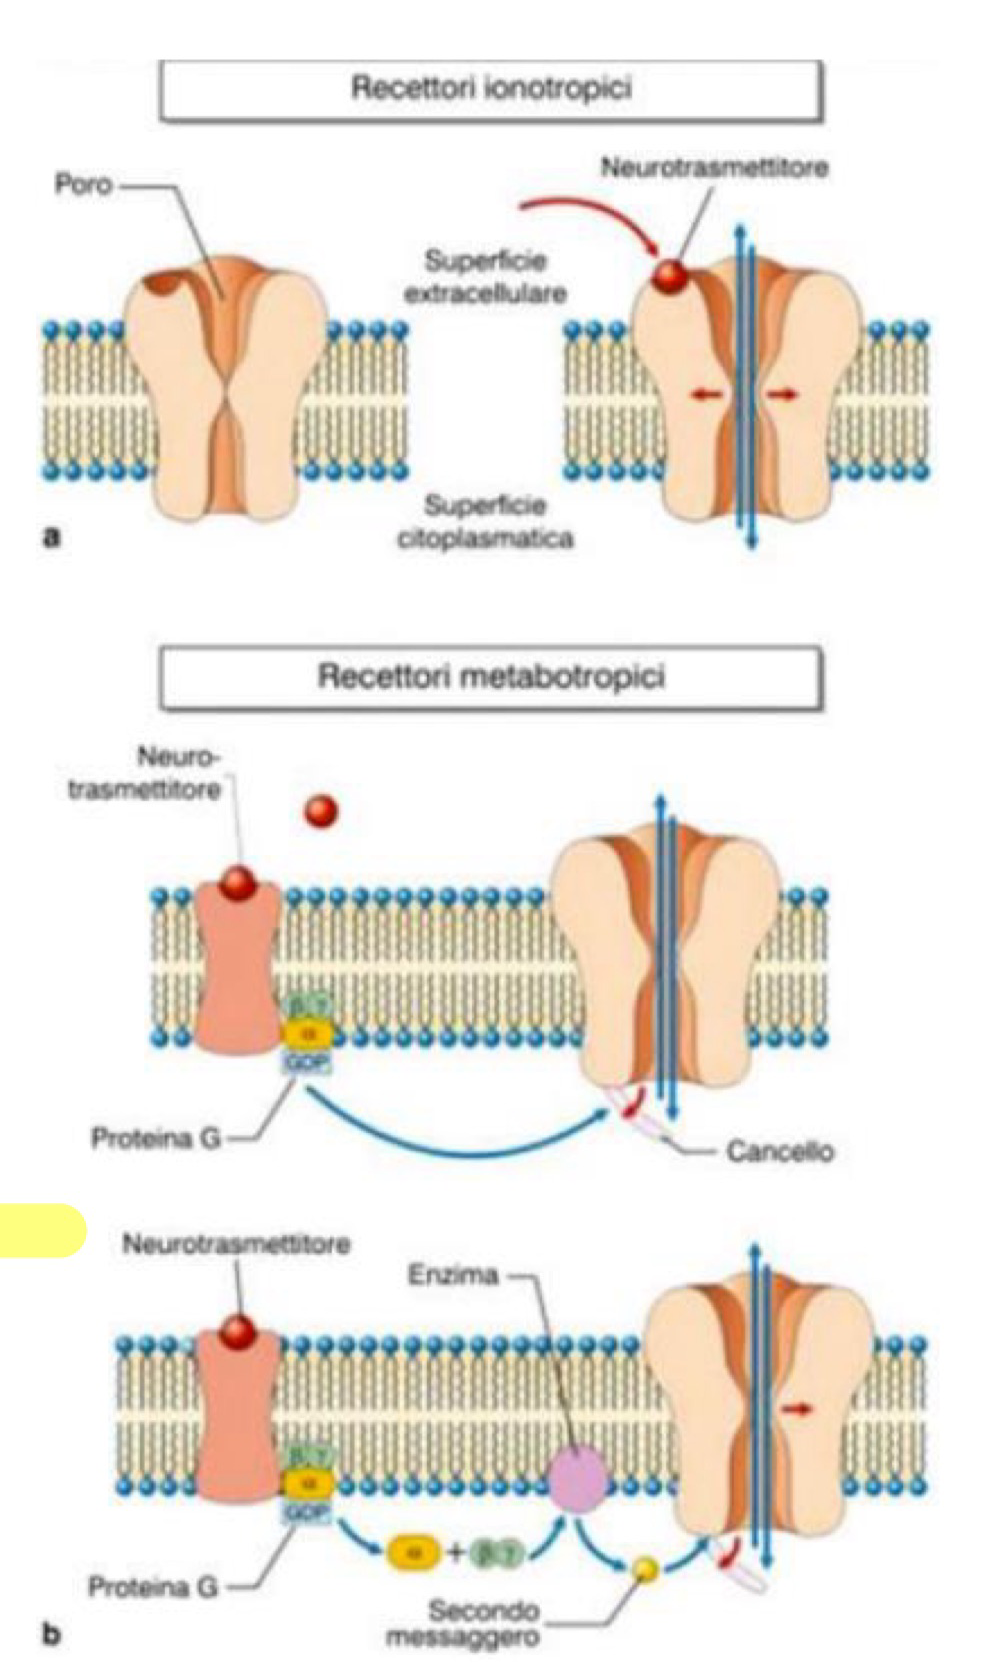
\includegraphics[width=\linewidth]{images/image25.png}
\end{wrapfigure}

Come abbiamo detto, i meccanismi di apertura dei canali possono essere di due tipi: ionotropico e metabotropico.
Nel meccanismo \textbf{ionotropico} il canale ionico può essere immaginato come una serratura e il neurotrasmettitore come la chiave: appena arriva, il neurotrasmettitore interagisce direttamente con il canale e lo apre. In questo caso il recettore coincide con il canale stesso o si trova su di esso. Si tratta quindi di un meccanismo semplice e molto rapido (sia ad attivare che a riattivare il canale, per esempio il riflesso motorio).
Nel meccanismo \textbf{metabotropico}, invece, il processo è più complesso, perché c’è una mediazione tra il legame del neurotrasmettitore e l’apertura del canale. Possiamo immaginarlo come aprire una porta tramite un citofono: il neurotrasmettitore non si lega al canale ma a un recettore separato. Questo legame genera delle molecole dette secondi messaggeri, che si muovono all’interno della cellula e interagiscono con i canali a cancello, inducendone l’apertura. Questo meccanismo è più lento e complesso, ma consente un’ampia gamma di funzioni e comporta cambiamenti nel tempo (plasticità, esperienza, apprendimento e memoria).

\begin{figure}[H]
    \centering
    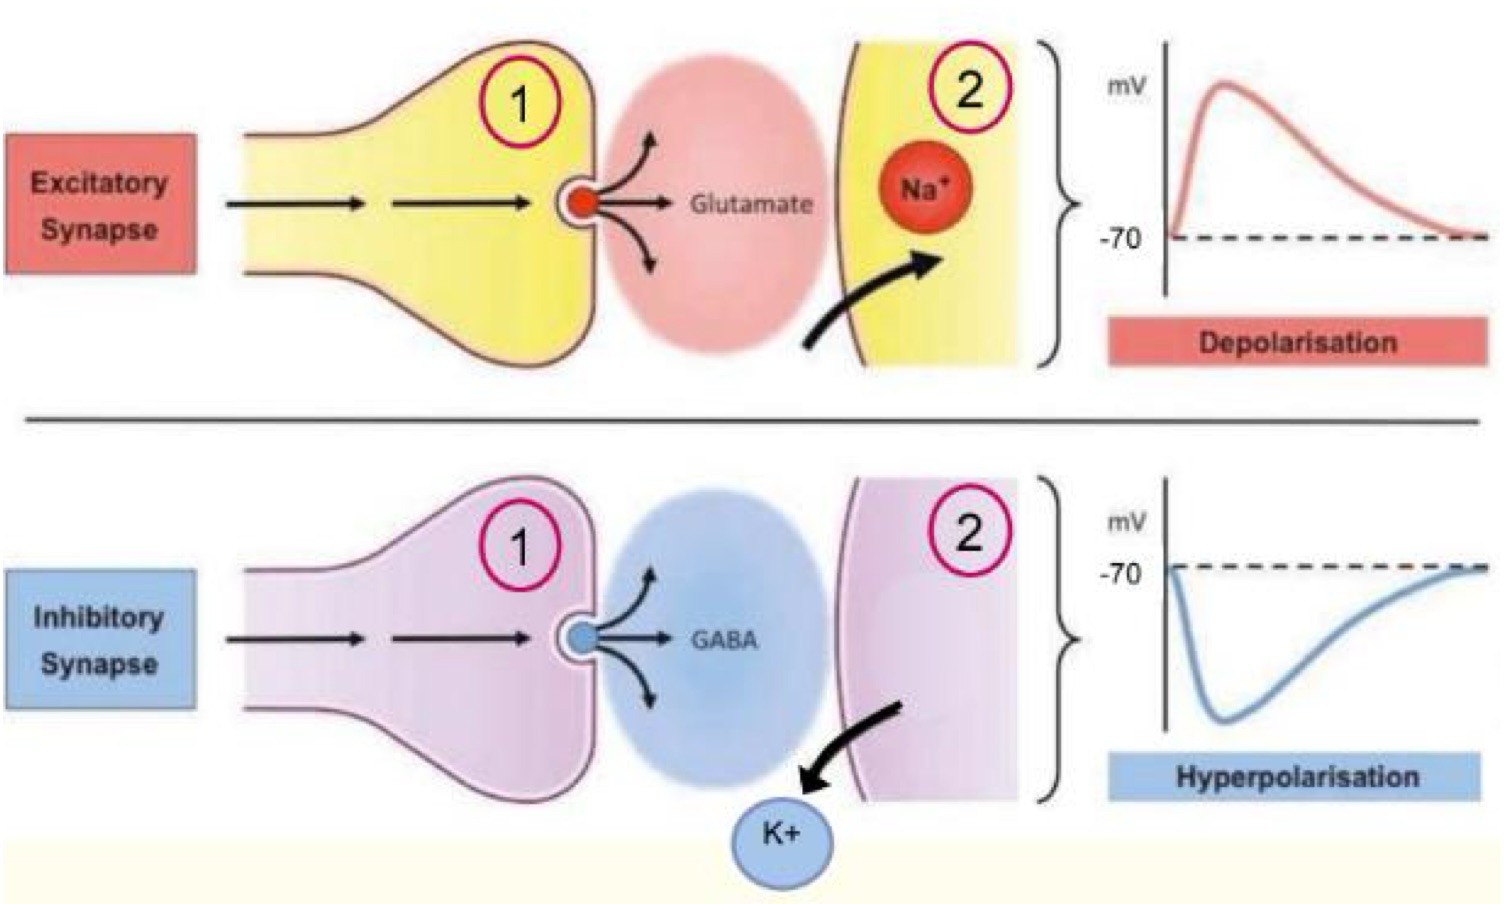
\includegraphics[width=0.65\textwidth]{images/image27.jpeg}
\end{figure}

Nelle sinapsi elettriche, poiché l’informazione è sempre una depolarizzazione (potenziale d’azione), l’unico effetto possibile sulla membrana post-sinaptica è una depolarizzazione: il segnale non può mai cambiare segno. Le sinapsi chimiche, invece, sono molto più flessibili e permettono una varietà di interazioni tra cellule. I vantaggi principali sono due: consentono variazioni del potenziale di membrana post-sinaptico sia in senso positivo sia in senso negativo, e permettono meccanismi di memoria.
Per quanto riguarda il primo vantaggio, consideriamo due casi. Nella prima situazione, quando un potenziale d’azione raggiunge il bottone sinaptico, viene rilasciato un neurotrasmettitore come il glutammato, che apre canali chimicamente controllati del sodio (sia ionotropici sia metabotropici). Questi canali sono passivi e permettono l’ingresso del sodio dall’esterno all’interno secondo gradiente elettrochimico, producendo una depolarizzazione della membrana post-sinaptica. Questa depolarizzazione è più lenta e meno ampia rispetto a un potenziale d’azione, e prende il nome di potenziale post-sinaptico eccitatorio (EPSP). È detto “eccitatorio” perché avvicina il potenziale di membrana alla soglia di apertura dei canali voltaggio-dipendenti del sodio, contribuendo così alla generazione di un potenziale d’azione, anche se da solo potrebbe non bastare.

Nel secondo caso, quando un potenziale d’azione raggiunge il bottone sinaptico, viene rilasciato un altro neurotrasmettitore, ad esempio il GABA, che apre i canali chimicamente controllati del potassio, esso tende a uscire dalla cellula post-sinaptica, producendo un’iperpolarizzazione della membrana. Il potenziale che ne deriva prende il nome di potenziale post-sinaptico inibitorio (IPSP), perché allontana il potenziale di membrana dalla soglia necessaria e quindi sfavorisce la generazione di un potenziale d’azione.
In sintesi, un potenziale post-sinaptico può essere eccitatorio o inibitorio a seconda dei canali che si aprono. Se si aprono i canali del sodio, si parla di sinapsi eccitatoria; se si aprono canali che hanno effetto iperpolarizzante, come quelli del potassio, si parla di sinapsi inibitoria. Anche il cloro partecipa in alcune sinapsi chimiche con canali chimicamente controllati: in genere ha effetto inibitorio, ma non in modo assoluto. Il potenziale di equilibrio del cloro è circa -65 mV, molto vicino al potenziale di membrana a riposo.

Infine, \textbf{cosa succede esattamente nella cellula post-sinaptica?}
Quando il potenziale d’azione arriva al neurone pre-sinaptico, si ha una forte depolarizzazione della membrana che apre i canali del calcio. L’ingresso di calcio provoca il rilascio del neurotrasmettitore nella fessura sinaptica. Dall’altro lato, i recettori della cellula post-sinaptica riconoscono quella specifica molecola e, attraverso meccanismi ionotropici o metabotropici, inducono l’apertura dei canali ionici chimicamente controllati. Gli ioni, muovendosi secondo gradiente elettrochimico, determinano una variazione del potenziale: può essere depolarizzazione (se entra sodio) o iperpolarizzazione (se esce potassio).

L’iperpolarizzazione, cioè un contributo negativo, ha un ruolo importante. Infatti la cellula post-sinaptica non riceve un solo potenziale, ma moltissimi, e non da una sola sinapsi, ma da tante contemporaneamente. Anche considerando una sola sinapsi, il neurone non riceve un singolo impulso, ma una sequenza di potenziali d’azione a distanza variabile. L’informazione, quindi, risulta dalla somma e dall’integrazione di tanti segnali eccitatori e inibitori.
L’esistenza delle sinapsi inibitorie è fondamentale, perché interviene nella terza funzione della cellula, ovvero l’integrazione dell’informazione, che possiamo considerare come l’elaborazione dei segnali ricevuti. Integrare significa sommare: la cellula somma tutte le informazioni che riceve, e il risultato di questa somma costituisce una decisione. Questo processo avviene fisicamente grazie alla membrana cellulare, che ricopre l’albero dendritico e il soma fino al cono d’emergenza.

\section{Sommazione spaziale e temporale}

La sommazione avviene tramite due meccanismi: \textbf{sommazione spaziale} e \textbf{sommazione temporale}.
Per quanto riguarda la sommazione, si parte dai potenziali post-sinaptici, sia eccitatori sia inibitori. Per la cellula ricevente, l’informazione si manifesta come una variazione del potenziale di membrana in un punto specifico: in un punto si può avere una depolarizzazione di un certo valore, in un altro punto un’altra depolarizzazione, e così via.

\begin{figure}[H]
    \centering
    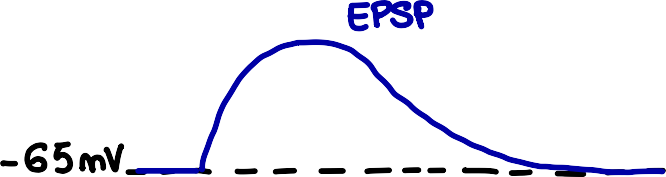
\includegraphics[width=0.80\textwidth]{images/image29.png}
\end{figure}

Per comprendere il processo, consideriamo un caso teorico con una sola sinapsi e un solo potenziale d’azione. In un punto della membrana post-sinaptica arriva un potenziale d’azione e si verifica una sinapsi eccitatoria: il potenziale di membrana passa dal valore di riposo (-65 mV) a una variazione positiva di pochi millivolt. Questa ampiezza è troppo piccola per raggiungere la soglia necessaria all’apertura dei canali voltaggio-dipendenti (circa 1 mV).
Dopo un breve intervallo, in assenza di altre perturbazioni, la membrana ritorna all’equilibrio grazie alle pompe sodio-potassio. In pratica, i canali si chiudono, il potenziale d’azione fa entrare ioni sodio, i canali poi si richiudono, e la pompa sodio-potassio ripristina l’equilibrio spostando dentro ioni potassio e fuori ioni sodio. L’intero processo richiede circa 10--15 millisecondi.
Nella realtà, però, si hanno tante sinapsi. Valutiamo quindi i meccanismi che avvengono.

\subsection*{Sommazione spaziale}

La sommazione spaziale si verifica quando più sinapsi eccitatorie, poste in punti vicini nello spazio, producono perturbazioni che si propagano nelle regioni circostanti e finiscono per agire insieme.

\begin{figure}[H]
    \centering
    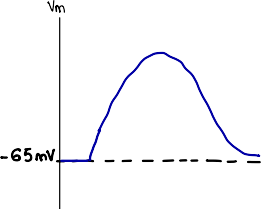
\includegraphics[width=0.80\textwidth]{images/image34.png}
\end{figure}

In questo caso gli ioni positivi entrano attraverso ciascuna sinapsi e la quantità totale di cariche positive all’interno della membrana risulta moltiplicata rispetto a quella prodotta da una sola sinapsi. Di conseguenza, l’ampiezza della curva che descrive il fenomeno è maggiore, e cresce ulteriormente se le sinapsi coinvolte sono numerose, ad esempio un centinaio. Questo avviene perché i potenziali post-sinaptici hanno una durata molto più lunga rispetto a quella del potenziale d’azione: prima che tornino all’equilibrio, c’è tempo per l’arrivo di numerosi potenziali d’azione. Si parla dunque di meccanismo spaziale, nel quale la cellula somma in modo passivo gli effetti generati da più sinapsi vicine.
Se però tra queste sinapsi ve ne sono anche di tipo inibitorio, l’effetto cambia. Nel caso di due sinapsi eccitatorie e una inibitoria, le cariche negative introdotte da quest’ultima si sommano a quelle positive delle prime, con un risultato finale meno marcato rispetto alla sommazione di tre eccitatorie. Se invece sono presenti due sinapsi inibitorie e una eccitatoria, il risultato è un’iperpolarizzazione.
Infine, la distanza della sinapsi dal cono d’emergenza dell’assone è un fattore importante. Una sinapsi lontana produce un effetto molto più debole rispetto a una vicina, perché durante il trasporto e la sommazione l’informazione può attenuarsi o perdersi. Diventano quindi fondamentali la geometria e l’estensione fisica della cellula nel determinare l’efficacia della sommazione spaziale.

\subsection*{Sommazione temporale}

La sommazione temporale dipende dal fatto che i potenziali d’azione arrivano sulla stessa sinapsi in sequenza, più o meno ravvicinati nel tempo.
Supponiamo di avere una sinapsi eccitatoria su cui arrivano tre potenziali d’azione molto vicini tra loro. Se ne arrivasse solo uno, si osserverebbe un singolo andamento del potenziale post-sinaptico, ma quando sono più di uno, il secondo potenziale arriva mentre il primo è ancora in corso, quindi la membrana non è tornata al riposo. In questo modo il secondo potenziale si somma al primo, causando un ulteriore aumento della depolarizzazione, in un meccanismo graduato. Lo stesso avviene con il terzo potenziale: ciascuno arriva su una membrana già parzialmente polarizzata, amplificando l’effetto complessivo. Alla chiusura dei canali ionici, infine, la membrana torna all’equilibrio.
Se la sinapsi fosse inibitoria, il grafico sarebbe lo stesso ma invertito, mostrando iperpolarizzazione anziché depolarizzazione. Se invece i potenziali d’azione arrivano distanziati nel tempo, la sommazione non si verifica perché ciascun potenziale ha il tempo di riportare la membrana al riposo prima dell’arrivo del successivo.

\subsection*{Combinazione di sommazione spaziale e temporale}

Si consideri una cellula post-sinaptica con due sinapsi: quella in alto, eccitatoria, e quella in basso, inibitoria. Immaginiamo di misurare i potenziali di membrana con tre elettrodi posti lungo lo stesso asse temporale: uno in alto sulla cellula pre-sinaptica della sinapsi eccitatoria, uno nel mezzo sulla cellula che fa la sinapsi inibitoria e uno in basso sulla cellula ricevente. In questo esempio, sulla cellula eccitatoria arrivano quattro potenziali d’azione e uno solo sulla sinapsi inibitoria.
All’inizio arriva un potenziale eccitatorio isolato, che non si somma con altri e porta la membrana a tornare rapidamente all’equilibrio. Successivamente, due potenziali d’azione ravvicinati sulla sinapsi eccitatoria si sommano temporalmente, aumentando il potenziale post-sinaptico fino a raggiungere la soglia dei canali del sodio voltaggio-dipendenti e generando un potenziale d’azione. Quando arriva simultaneamente un potenziale eccitatorio e uno inibitorio, i due effetti si bilanciano tra loro, annullandosi quasi completamente.
In questo modo, i meccanismi di sommazione temporale e spaziale agiscono insieme: l’effetto della sommazione temporale si somma spazialmente con quello di altre sinapsi. Moltiplicando questo fenomeno per migliaia di sinapsi e per un numero elevatissimo di potenziali d’azione nel tempo, si ottiene una variazione del potenziale post-membrana che può assumere forme molto diverse, senza un andamento tipico.
L’output binario della cellula è costituito dalla sequenza dei potenziali d’azione. Nell’esempio considerato, si osservano quattro sinapsi e quattro treni di potenziali diversi. L’informazione passa dalla cellula pre-sinaptica a quella post-sinaptica tramite una sinapsi chimica. Sulla membrana post-sinaptica si osserva quindi l’effetto della sommazione temporale o spaziale, il cui risultato è rappresentato nel grafico. L’intervallo temporale considerato è di circa 10 millisecondi.

\begin{figure}[H]
    \centering
    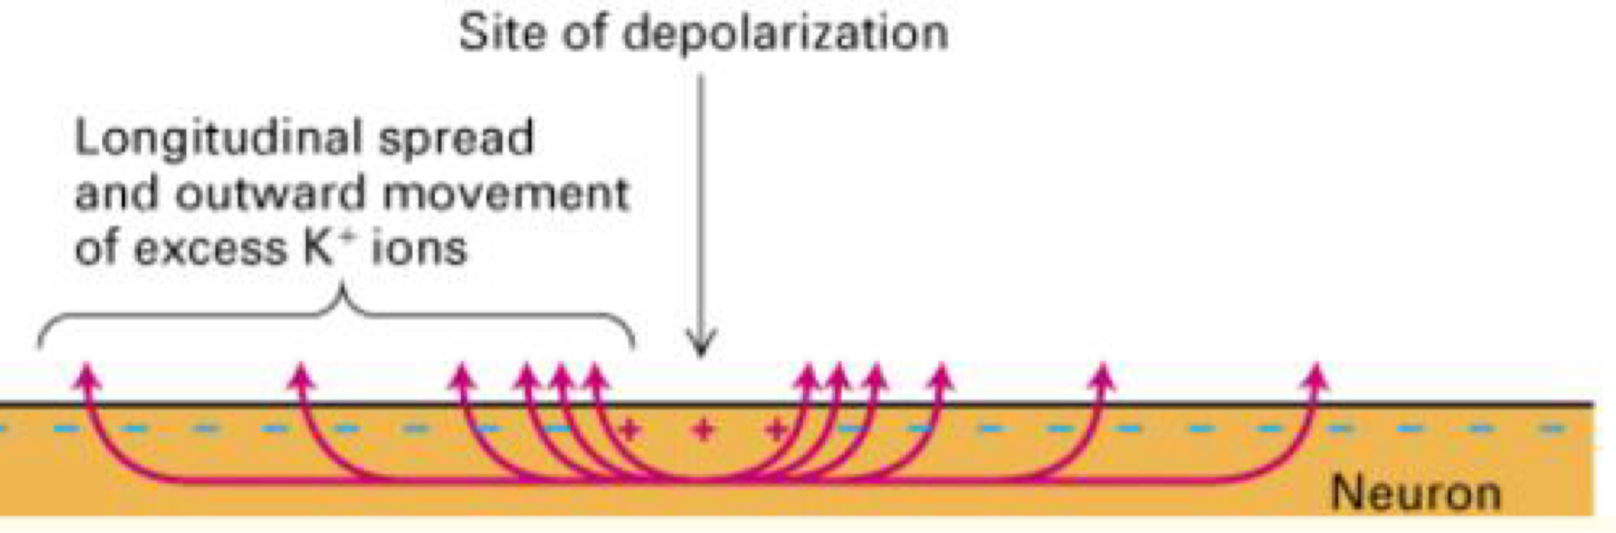
\includegraphics[width=0.80\textwidth]{images/image43.png}
\end{figure}

\subsection*{Propagazione e potenziali graduati}

Le perturbazioni di cui si è parlato in precedenza corrispondono ai potenziali post-sinaptici sommati tra loro, che producono una variazione del potenziale di membrana. Localmente si osserva una depolarizzazione: la membrana in quella zona diventa meno negativa rispetto alle altre regioni, ma questo non significa che diventi positiva, semplicemente che la negatività è ridotta. Le cariche concentrate, essendo libere di muoversi nel liquido intracellulare, generano correnti intracellulari che propagano la perturbazione ai siti vicini. Questa propagazione è passiva, non direzionata e dipende dalla distanza dal punto di origine del potenziale. Grazie a questo meccanismo, la sommazione spaziale può avvenire anche quando le sinapsi non sono direttamente adiacenti tra loro, e permette al risultato finale di raggiungere il cono d’emergenza dell’assone.
I potenziali post-sinaptici sommati tra loro prendono il nome di \textbf{potenziali graduati}. I potenziali d’azione hanno sempre lo stesso segno positivo e risultano quindi sempre depolarizzanti, a differenza dei potenziali graduati, che possono essere sia depolarizzanti che iperpolarizzanti. Perché si generi un potenziale d’azione è necessario raggiungere un valore soglia, mentre nei potenziali graduati questo non è richiesto. I potenziali d’azione eseguono il principio del tutto o nulla, mentre negli altri l’intensità dello stimolo influisce sull’ampiezza del segnale. Per quanto riguarda la propagazione, i potenziali d’azione si diffondono in maniera continua o saltatoria, i graduati invece si propagano solo passivamente e non si rigenerano mai, percorrendo distanze minori. Inoltre i potenziali d’azione presentano un periodo refrattario assoluto e un periodo refrattario relativo, assenti in quelli graduati. I potenziali d’azione caratterizzano in modo specifico le cellule eccitabili, come quelle nervose, muscolari e cardiache, mentre i graduati possono essere presenti in tutte le cellule.

\begin{figure}[H]
    \centering
    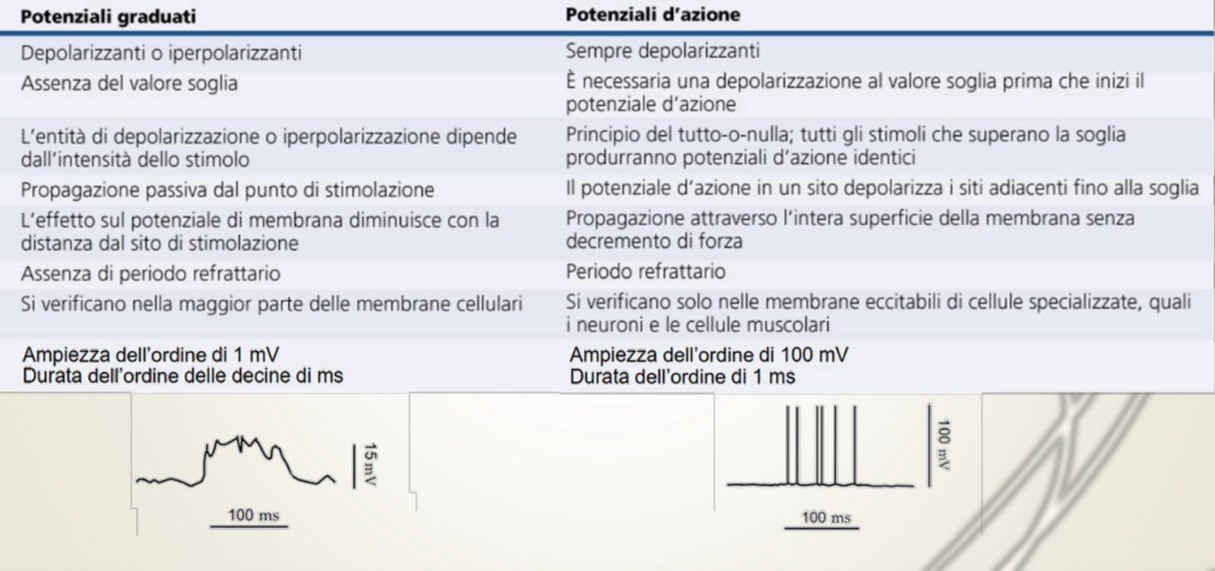
\includegraphics[width=0.80\textwidth]{images/image44.jpeg}
\end{figure}

\subsection*{Integrazione dell’informazione}

L’integrazione dell’informazione nella membrana avviene tramite la sommazione degli EPSP e degli IPSP, sia spaziale che temporale. Questo determina la depolarizzazione o l’iperpolarizzazione della membrana: se la depolarizzazione non raggiunge la soglia o se prevale l’iperpolarizzazione, il potenziale d’azione non si genera. Il segnale risultante si propaga passivamente fino al cono d’emergenza dell’assone, dove può nascere il potenziale d’azione. La possibilità di raggiungere la soglia dipende dall’intensità della perturbazione e dalla geometria dei dendriti, in particolare dalla loro distanza e posizione rispetto al cono d’emergenza, poiché l’effetto si attenua con la distanza.

\begin{figure}[H]
    \centering
    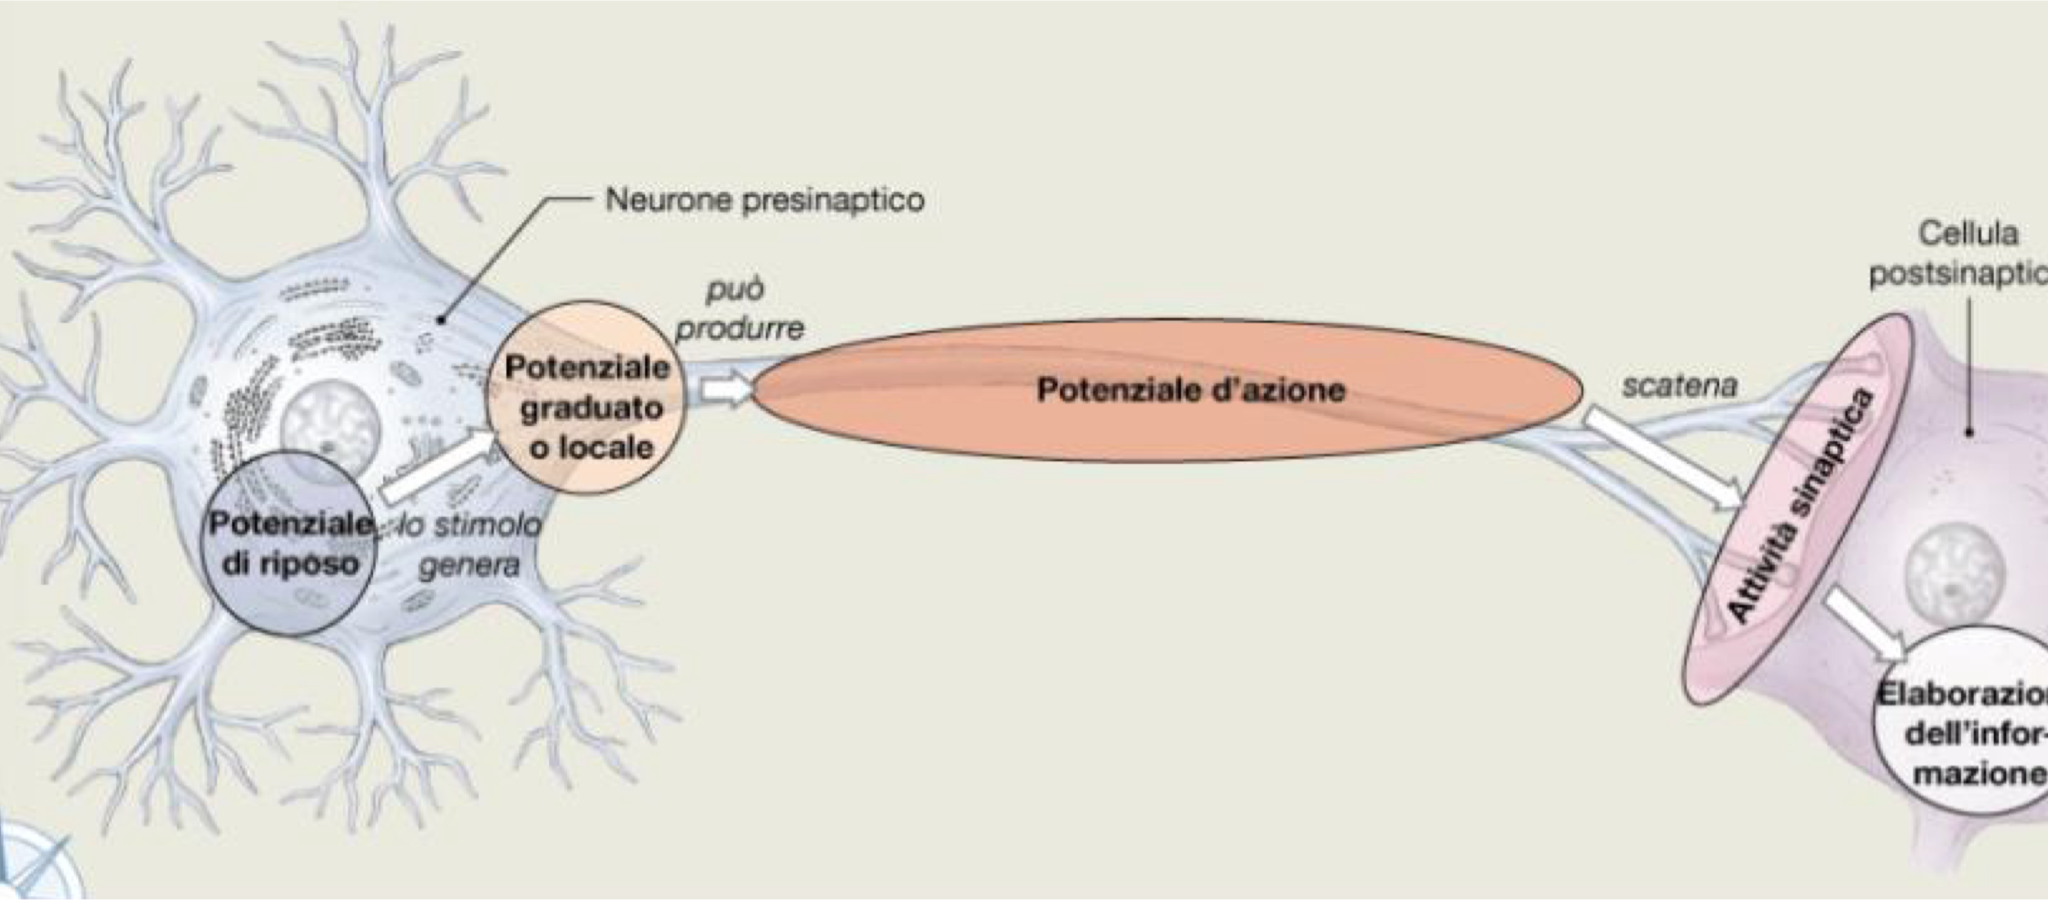
\includegraphics[width=0.80\textwidth]{images/image49.png}
\end{figure}

All’interno della cellula, che possiede un potenziale di riposo, gli stimoli ricevuti dai dendriti con segno positivo o negativo producono, tramite sommazione spaziale o temporale, un potenziale graduato o locale. Se questo potenziale supera la soglia, viene generato un potenziale d’azione, che si propaga lungo l’assone in maniera continua o saltatoria fino alla sua estremità. La cellula comunica con altre tramite sinapsi, di solito chimiche, che possono essere eccitatorie o inibitorie: in base al neurotrasmettitore rilasciato, si genera un potenziale d’azione eccitatorio o inibitorio nella cellula successiva.

\section{Registrazioni intra ed extra cellulari}

Le registrazioni intracellulari permettono di misurare direttamente il potenziale attraverso la membrana cellulare. Per farlo si utilizza un elettrodo di riferimento, posizionato all’esterno, e un elettrodo perforante, che deve acquisire il potenziale dall’interno della cellula. Questo può avvenire in due modi: perforando fisicamente la membrana con l’elettrodo e attraversandola, oppure utilizzando un elettrodo che si fonde con la membrana entrando in contatto elettrico con la cellula. L’elettrodo perforante è solitamente una micropipetta di vetro riempita di soluzione salina concentrata, al cui interno vengono inseriti fili metallici collegati a un oscilloscopio. Quest’ultimo permette di visualizzare l’ampiezza del potenziale di membrana in Volt. Lo stesso avviene per l’elettrodo extracellulare: la differenza tra interno ed esterno della cellula rappresenta infatti il potenziale di membrana. Rispetto a un elettrodo patch, quello perforante è più complesso da utilizzare e presenta un rischio maggiore di danneggiare la membrana. Questo perché attraversarla senza comprometterla è un’operazione molto delicata: è più semplice in alcune zone della cellula, come nel soma o in certe parti dell’albero dendritico, e molto più difficile negli assoni o nelle ramificazioni sottili. A questa difficoltà si aggiunge il problema delle registrazioni in vivo, dove occorre raggiungere i neuroni nel cervello senza danneggiare il tessuto circostante. Le registrazioni intracellulari possono quindi essere effettuate in vivo, cioè direttamente nel cervello, oppure in vitro, estraendo i neuroni e studiandoli in laboratorio. In quest’ultimo caso, poiché i neuroni non si trovano più nel loro ambiente naturale, è necessario stimolarli artificialmente con iniezioni di corrente che simulano l’effetto delle sinapsi, così da osservare le loro risposte. Questo rappresenta un compromesso utile quando le registrazioni in vivo non sono possibili.
Il grande vantaggio delle registrazioni intracellulari è che consentono di misurare in modo diretto e preciso l’attività neuronale, cioè l’andamento nel tempo del potenziale di membrana. Dal punto di vista della qualità del segnale non esistono tecniche equiparabili: l’unico modo per avere una misura diretta dell’attività neuronale è proprio questo tipo di registrazione.

Le registrazioni extracellulari evitano l’aspetto più complesso delle registrazioni intracellulari, cioè l’attraversamento della membrana. Questo è possibile perché, quando nella cellula avvengono delle perturbazioni e si generano correnti intracellulari, all’esterno si creano correnti simmetriche ma di segno opposto. In questo modo, ponendo un elettrodo al di fuori della cellula e confrontandolo con un altro punto di riferimento, è possibile rilevare una differenza che indica che qualcosa sta accadendo, anche se in maniera meno chiara rispetto a quanto si osserva all’interno.
Il grande vantaggio di questa tecnica è che non si deve attraversare la membrana, evitando così il rischio di danneggiare la cellula. Non ci si scontra quindi con il problema delle porzioni sottili e fragili della membrana, e si può registrare vicino a strutture come assoni o dendriti. Anche in vivo l’operazione risulta più semplice. Lo svantaggio, invece, riguarda la qualità del segnale: con questa tecnica non si misura direttamente il potenziale di membrana, ma solo variazioni importanti di esso. Più grande è la variazione, più è probabile che venga rilevata anche con un elettrodo esterno. Questo significa che non si misura l’attività neuronale in senso stretto, ma si riescono a rilevare solo i fenomeni più intensi, cioè i potenziali d’azione, e non quelli graduati. Infatti, le variazioni dei potenziali graduati sono spesso così piccole da confondersi con il rumore, mentre quelle dei potenziali d’azione sono sempre evidenti e certe. Questa tecnica viene quindi utilizzata esclusivamente per rilevare l’avvenuto potenziale d’azione e per sapere in quale istante esso si verifica. Non si misura la sua ampiezza, ma non è un problema, perché il potenziale d’azione ha sempre la stessa grandezza. L’informazione non è contenuta nell’ampiezza o nell’andamento, ma nella frequenza con cui i potenziali d’azione appaiono. Ad esempio, se in un secondo si hanno cinque potenziali d’azione, nel caso in cui siano ravvicinati tra loro, a distanza di 3 millisecondi, si ha una sommazione temporale che produce un effetto maggiore sul neurone ricevente. Se invece sono distanziati, l’effetto risulta più blando.
In sintesi, quando si vuole studiare l’attività dei potenziali d’azione ci sono due possibilità: se si vogliono indagare i meccanismi di generazione del potenziale, occorre misurarne l’andamento nel tempo, e quindi non si possono usare le registrazioni extracellulari, ma servono quelle intracellulari, come nel classico esperimento sull’assone gigante. Se invece non si è interessati all’ampiezza o all’andamento, ma solo a verificare se una cellula in un certo momento stia producendo o meno un potenziale d’azione, allora la registrazione extracellulare è sufficiente. Questo non vale per i potenziali graduati, perché troppo piccoli per essere rilevati con questa tecnica.

\begin{figure}[H]
    \centering
    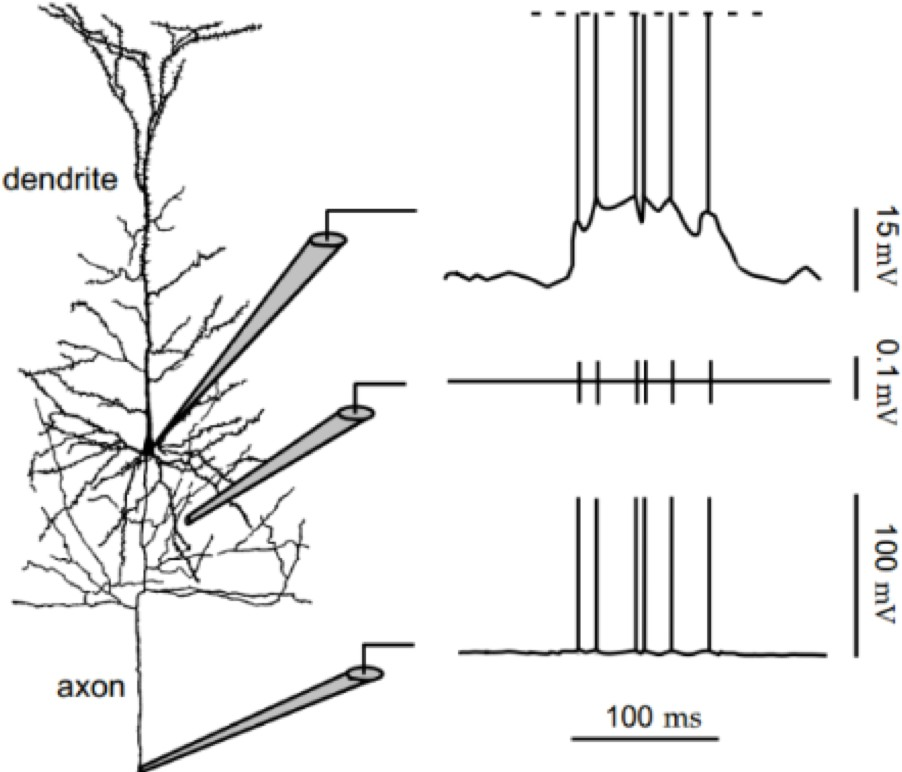
\includegraphics[width=0.80\textwidth]{images/image50.jpeg}
\end{figure}

In figura è rappresentato un neurone piramidale, così chiamato perché il soma ha una forma piramidale. Sono state effettuate tre registrazioni simultanee sullo stesso neurone, confrontando i risultati.
La prima registrazione è intracellulare e viene fatta sul soma, vicino al cono di emergenza dell’assone. In questo punto è possibile misurare sia i potenziali d’azione sia i potenziali graduati, perché l’elettrodo entra direttamente in contatto con l’interno della cellula. Nel grafico, i potenziali d’azione appaiono tagliati a causa della scala utilizzata. La seconda registrazione è extracellulare. Qui l’elettrodo viene posto vicino all’assone e permette di rilevare con precisione gli istanti in cui si verificano i potenziali d’azione, ma non di misurarne l’ampiezza reale. Inoltre, i potenziali graduati non vengono registrati, perché l’elettrodo non è abbastanza sensibile. In questo caso, nel grafico l’ampiezza rilevata è di circa 0,1 mV, molto più piccola di quella reale.
La terza registrazione è intracellulare, ma fatta direttamente sull’assone. In questo modo si entra a contatto con l’ambiente cellulare e si rilevano i potenziali d’azione, ma non i potenziali graduati. Confrontando i tre grafici, si osserva che le ampiezze registrate sono molto diverse tra loro: nella registrazione extracellulare, l’ampiezza appare molto ridotta rispetto al valore reale, quindi non si può dire di aver misurato effettivamente il potenziale. Inoltre, nell’assone non compaiono i potenziali graduati. Ciò che rimane uguale in tutte e tre le registrazioni è l’istante in cui i potenziali d’azione si verificano. Quando si devono effettuare delle registrazioni, la prima domanda da porsi è a cosa serva la misura. Se si vuole vedere se la cellula risponde a stimoli interni attraverso i potenziali graduati, la registrazione extracellulare deve essere esclusa. Se invece interessa solo verificare la presenza dei potenziali d’azione, allora la registrazione extracellulare può essere sufficiente. Un’altra considerazione riguarda il contesto: una registrazione in vivo è molto più difficile da realizzare rispetto a una in vitro. In conclusione, la scelta tra registrazione intracellulare o extracellulare dipende dalla localizzazione, dal tipo di segnale che si vuole acquisire e dalla possibilità o meno di stimolare il neurone. Per esempio, se si vuole osservare la risposta di una cellula a un certo stimolo e descrivere il trend dei potenziali che produce, si userà una registrazione extracellulare. Se invece si vogliono studiare i meccanismi di generazione del potenziale d’azione, sarà necessario ricorrere a una registrazione intracellulare in vitro.

\begin{figure}[H]
    \centering
    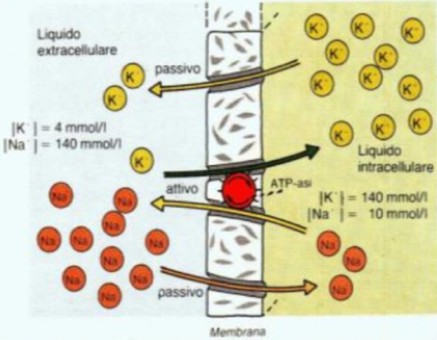
\includegraphics[width=0.80\textwidth]{images/image51.jpeg}
\end{figure}
\chapter{Modelli elettrici della membrana neuronale}

\section{Introduzione ai modelli elettrici di membrana}

Le caratteristiche fisiche della membrana cellulare possono essere tradotte in proprietà
elettriche, utilizzando dei \textbf{circuiti elettrici come rappresentazione astratta di fenomeni }che, nella realtà, hanno natura fisica. Questo tipo di modello risulta uno strumento adeguato a rappresentare la membrana di cellule eccitabili in quanto, quest'ultima, svolge le proprie funzioni tramite la \textbf{variazione di grandezze elettriche }(come il potenziale di membrana o la corrente di membrana).

Le correnti ioniche che attraversano la membrana possono essere attivate da:

\begin{itemize}
  \item \textbf{Canali di membrana}: non selettivi, selettivi o controllati (a cancello). Possono essere \textit{canali variabili }in base a specifici stimoli o \textit{canali sempre aperti}, che permettono il passaggio di ioni secondo gradiente elettrochimico (trasporto passivo);
  \item \textbf{Pompe ioniche}: dove, invece, gli ioni vengono spostati contro gradiente di concentrazione, utilizzando energia (trasporto attivo).
\end{itemize}
\textbf{LIVELLO DI ASTRAZIONE}

L'obiettivo principale è quello di \textbf{passare dalla struttura reale del neurone }(in figura 1) \textbf{ad un modello di esso }(in figura 4), che ovviamente non dovrà essere fedele al progetto fisico. Questo perché bisogna utilizzare uno schema utile ai nostri scopi, fornendo le informazioni corrette.
\subsection{Neurone biologico completo}
Viene rappresentato un neurone realistico, con tutti i suoi tratti fisiologici principali (soma, albero dendritico, assone e terminali assonici). Non è utile in questo caso perché è una struttura troppo complessa per poter essere modellata direttamente;
\subsection{Semplificazione a compartimenti}
Schematizzazione del neurone con \textbf{segmenti rettilinei }connessi tra loro, come rappresentazione delle ramificazioni dendritiche. Abbiamo poi le sinapsi ancora visibili, rappresentate da \textbf{triangolini }ed infine il colle dell'assone, rappresentato da un \textbf{cerchio};


\subsection{Modello semplificato a pochi rami}

Le precedenti ramificazioni dendritiche sono adesso rappresentate da \textbf{pochi rami principali }più grandi. Le sinapsi sono ancora visibili in quanto è necessario che l'informazione si propaghi;


\subsection{Modello a punto singolo (one-compartment model)}

Si arriva ad una situazione di estrema semplificazione, dove il cono di emergenza dell'assone è rappresentato da una \textbf{sfera }e le sinapsi si trovano tutte vicine tra loro \textbf{come se si fondessero in un unico punto}. Questo modello è detto ``\textbf{\textit{a}}\textbf{\textit{ }}\textbf{\textit{punto}}'' o ``\textbf{\textit{integratore}}'': non si considera più la distribuzione spaziale ma solo l'attività globale e tutte le sinapsi contribuiscono alla stessa variabile di membrana.

\subsubsection{Modello a singolo compartimento}

Il modello a singolo compartimento non è così tanto lontano dalla realtà, infatti, ricorda molto le \textit{registrazioni intracellulari}, dove il potenziale viene misurato solo in un punto del neurone, assumendo che esso rappresenti bene l'intero compartimento cellulare.
Si andranno a \textbf{trascurare le variazioni del potenziale di membrana nello spazio}, poiché sono state eliminate con la modellizzazione fatta in precedenza. A questo punto, quindi, è possibile descrivere le grandezze elettriche con un \textbf{unico valore rispetto alla dimensione spaziale}: un unico valore per il potenziale di membrana (costante nello spazio) e uno per le correnti di membrana.
Gli elementi circuitali equivalenti che verranno utilizzati nel modello sono:

\begin{itemize}
  \item Resistenza $\rightarrow$ canali ionici;
  \item Condensatore $\rightarrow$ capacità della membrana di accumulare cariche.
\end{itemize}
\textbf{OSS: }per svincolarsi dalle dimensioni della membrana ogni grandezza elettrica sarà per ora riferita all'unità di spazio.

\subsubsection{Proprieta' capacitive della membrana}

La membrana è costituita da un \textbf{doppio strato fosfolipidico }che separa due ambienti con distribuzione di cariche differenti: \textbf{cariche negative }disposte all'interno della membrana e \textbf{cariche positive }all'esterno.
Il comportamento elettrico del doppio strato fosfolipidico può essere modellizzato con un \textbf{condensatore}, infatti, si osservano due superfici separate da una \textit{distanza d }(spessore del doppio strato fosfolipidico) su cui supponiamo essere distribuite le cariche dell'ambiente intra ed extra-cellulare.
Per svincolarsi dalla dimensione spaziale, nel circuito è conveniente, anziché calcolare la capacità del condensatore, dividere quest'ultima per la superficie della membrana (A): si ottiene così la \textbf{capacità specifica di membrana}.

\[
  C_m = c_m \cdot A
\]
\begin{itemize}
  \item $C_m$: capacità di membrana (nF)
\end{itemize}
\begin{figure}[H]
  \centering
  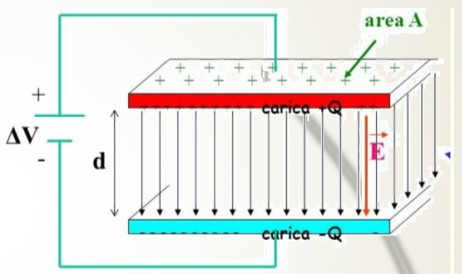
\includegraphics[width=0.80\textwidth]{images/image54.jpeg}
\end{figure}

\[
  c_m = \frac{C_m}{A}
\]
\begin{itemize}
  \item $c_m$: capacità specifica di membrana ($\mathrm{\mu F/cm^2}$)
\end{itemize}
\textbf{EQUAZIONE DI BASE DELLA MEMBRANA}

A questo punto è possibile iniziare a scrivere l'\textit{equazione di base }del circuito che stiamo andando a considerare partendo appunto dal condensatore.

\[
  I = \frac{dQ}{dt} = C_m \frac{dV}{dt}
\]

La corrente I in questo caso è quella generata dalla differenza di potenziale $\Delta V$ (costante nello spazio, ma non nel tempo), che occorre che passi attraverso una membrana di capacità totale $C_m$ per cambiare la tensione V ad una velocità $dV/dt$.

\subsubsection{Proprieta' resistive della membrana}

Il comportamento elettrico della membrana dipende principalmente dall'attività dei canali ionici e delle pompe ioniche. Infatti, un canale di membrana che permette il passaggio di ioni, quindi di corrente, si può immaginare rappresentato con delle \textbf{resistenze/conduttanze}.
Se si hanno più canali aperti, si avrà una \textbf{bassa resistenza}, se invece si hanno più canali chiusi, la \textbf{resistenza }sarà \textbf{infinita}.
\textbf{OSS: }si spiega così anche l'effetto dei farmaci/tossine che bloccano i canali, infatti, la loro azione, aumenta la resistenza della membrana ostacolando la trasmissione nervosa.

\begin{itemize}
  \item \textbf{Resistenza}: determina quanta corrente I è necessaria per mantenere, a regime, una differenza di potenziale $\Delta V$;
  \item \textbf{Conduttanza}: direttamente proporzionale alla superficie di membrana A.
\end{itemize}
Anche in questo caso si andranno ad utilizzare le grandezze specifiche, per cui la conduttanza sarà divisa per la superficie di membrana A, mentre la resistenza moltiplicata per essa.

\[
  G_m = g_m \cdot A
\]
\begin{itemize}
  \item $G_m$: conduttanza di membrana (S)
\end{itemize}
\[
  g_m = \frac{G_m}{A}
\]
\begin{itemize}
  \item $g_m$: conduttanza specifica di membrana ($\mathrm{S/m^2}$)
\end{itemize}
\[
  R_m = \frac{r_m}{A}
\]
\begin{itemize}
  \item $R_m$: resistenza di membrana (M$\Omega$)
\end{itemize}
$r_m = R_m \cdot A$ $\rightarrow$ \textit{Resistenza specifica di membrana} ($\Omega\,\text{m}^2$)

\textbf{EQUAZIONE DI NERST -- richiamo}

Per ciascuna famiglia ionica è possibile confrontare il potenziale di riferimento con il potenziale di membrana per capire la spinta che agisce sugli ioni: se il \textbf{potenziale }di riferimento è \textbf{più negativo }si parla di effetto \textbf{\textit{iperpolarizzante}}, se è \textbf{meno negativo }si parla invece di effetto \textbf{\textit{depolarizzante}}.
Oltre a questo, il potenziale elettrochimico può essere utilizzato per capire l'effetto di una corrente ionica: \textbf{il potenziale di equilibrio tende a spostare la membrana verso quel}

\begin{figure}[H]
  \centering
  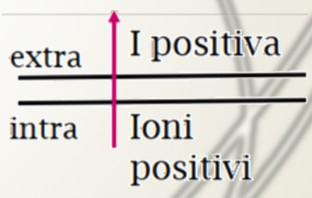
\includegraphics[width=0.80\textwidth]{images/image56.jpeg}
\end{figure}

valore. 1, è il potenziale con cui le forze di diffusione secondo gradiente di concentrazione bilanciano quelle secondo gradiente elettrico di tipo j.

\begin{itemize}
  \item V < E: correnti ioniche positive verso l'interno della membrana $\rightarrow$ depolarizzazione;
  \item V > E: correnti positive verso l'esterno della membrana $\rightarrow$
\end{itemize}
iperpolarizzazione/ripolarizzazione;

\begin{itemize}
  \item Sinapsi eccitatorie: $V_{\text{th}}$ < E (depolarizzanti)
  \item Sinapsi inibitorie: $V_{\text{th}}$ > E (iperpolarizzanti)
\end{itemize}
La differenza di potenziale elettrico tra l'interno e l'esterno della cellula viene originata da gradienti ionici, mantenuta dalle pompe ioniche e rappresenta una forza elettromotrice proprio come una pila.

\subsubsection{Corrente di membrana}

La \textbf{corrente di membrana }rappresenta il movimento netto di cariche elettriche (ioni) che attraversano la membrana cellulare, in entrata o in uscita dalla cellula.

\begin{itemize}
  \item \textbf{Positiva }$\rightarrow$ ioni positivi \textbf{escono }dalla cellula;
  \item \textbf{Negativa }$\rightarrow$ ioni positivi \textbf{entrano }nella cellula.
\end{itemize}
\textbf{N.B. }se si parla di ioni negativi la direzione è opposta.

Come già anticipato, attraverso la membrana si hanno diversi tipi di correnti date dai canali ionici, che possono essere sommate tutte insieme e rappresentate proprio dalla corrente di membrana:
\[
  i_m = \sum_j g_j\,(V - E_j)
\]
\begin{itemize}
  \item $g_j$ $\rightarrow$ \textit{conduttanza specifica dello ione di tipo j}
  \item $g_j(V - E_j)$ $\rightarrow$ \textit{corrente dovuta ai canali di tipo j}
  \item $E_j$ $\rightarrow$ \textit{potenziale di equilibrio per cui le forze di diffusione secondo gradiente bilanciano quelle secondo gradiente elettrico per gli ioni di tipo j.}
\end{itemize}
\textbf{OSS:} anche in questo caso ci si riferisce all'unità di superficie; le grandezze sono normalizzate per unità di superficie di membrana.

\subsubsection{Conduttanze di membrana}

In generale le conduttanze di membrana possono essere suddivise in:

\begin{itemize}
  \item \textbf{Conduttanze costanti nel tempo}: dovute alle \textbf{pompe ioniche }o ai \textbf{canali ionici }\textit{sempre aperti }(rappresentati da resistore + generatore). Le prime sono \textit{sempre attive}, ma \textbf{non vale l'equazione di Nerst }in quanto spostano ioni contro gradiente; possono comunque essere rappresentate con rami resistivi senza generatore.
  \item \textbf{Conduttanze variabili nel tempo}: questo accade perché molti canali ionici si aprono o si chiudono in risposta a \textbf{variazioni di potenziale }(\textit{canali voltaggio-dipendenti}) o a
\end{itemize}
\begin{figure}[H]
  \centering
  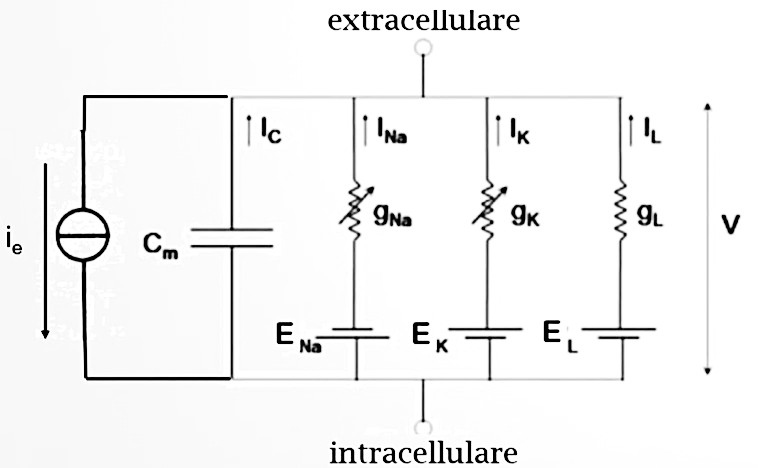
\includegraphics[width=0.80\textwidth]{images/image58.jpeg}
\end{figure}

stimoli chimici (canali chimicamente controllati, come quello del cloro). Sono conduttanze in funzione del potenziale di membrana (V).
I rami costanti, proprio a causa della conduttanza invariante in funzione del tempo, possono essere raggruppati in un unico ramo equivalente, il \textbf{ramo di leakage}, formato da un \textbf{resistore di leakage }e da un \textbf{generatore di tensione }(che rappresenta la spinta elettrochimica costante).
Se tutti i canali sono chiusi e restano attivi solo i fenomeni di leakage, la membrana è in

\textit{equilibrio elettrico }e il potenziale di membrana è quello di riposo (-70 mV).

Le correnti dovute alle conduttanze costanti sono detti ``\textbf{correnti di perdita}'' (\textit{leakage currents}):
\[
  i_L = g_L\,(V - E_L)
\]
\begin{itemize}
  \item $g_L$ $\rightarrow$ \textit{conduttanza di perdita (fissa e riferita al ramo di leakage)}
  \item $V$ $\rightarrow$ \textit{potenziale di membrana}
  \item 1/ $\rightarrow$ \textit{potenziale di equilibrio }(valore medio o ``efficace'' per più ioni)
\end{itemize}
Queste correnti rappresentano il \textbf{flusso costante di ioni che attraversa la membrana }anche in assenza di stimoli, quindi, quando tutti i canali a cancello (voltaggio-dipendenti o chimico-dipendenti) sono chiusi. Sono correnti sempre presenti, anche a riposo.

\subsubsection{La membrana come circuito elettrico}

Quindi, arrivati a questo punto e riassumendo tutto ciò che abbiamo visto fino ad adesso, è possibile modellizzare tutti i fenomeni bioelettrici con componenti circuitali.

\begin{itemize}
  \item \textbf{DiPerenza di potenziale ai lati della membrana = generatore di tensione}
  \item \textbf{Corrente ionica attraverso la membrana = corrente I (che fluisce nel ramo)}
  \item \textbf{Canali ionici = resistori}
  \item \textbf{Doppio strato fosfolipidico = condensatore}
\end{itemize}
\textbf{ESEMPIO DI CIRCUITO EQUIVALENTE DI MEMBRANA}

Riassumiamo il tutto con un circuito rappresentativo: si hanno l'ambiente extra-cellulare ed intra-cellulare ai lati opposti del circuito e nel mezzo vengono posti tanti rami in parallelo quanti sono i fenomeni che si vogliono
rappresentare. In particolare, si ha un numero variabile di rami che rappresentano tutto ciò che non si può inserire nel ramo di leakage, ovvero tutto ciò che non varia nel tempo, come ad esempio i canali ionici voltaggio-dipendenti, uno per ramo, in quanto hanno una \textbf{evoluzione temporale diversa}.
OSS: come si può notare si hanno due rami, quello del sodio e quello del potassio, con conduttanza variabile nel tempo. I due generatori di tensione dipendono dal potenziale elettrochimico ed infatti sono opposti nei due rami $\rightarrow$ potenziali di segno opposto. Ma il generatore del potassio e quello di membrana hanno lo stesso verso in quanto sono entrambi negativi.

\begin{itemize}
  \item \textbf{Condensatore }:0\textbf{: }capacità di membrana di accumulare cariche.
  \item \textbf{Generatori di tensione };12, ;3, ;4: forze elettromotrici corrispondenti ai potenziali di Nerst e alle correnti di perdita. Spingono gli ioni a muoversi secondo il gradiente elettrochimico.
  \item \textbf{Resistenze/conduttanze }=12, =3, =4: canali ionici, -56 > -7 dipendono dal potenziale di membrana, mentre, -/ è costante e rappresenta i canali di perdita sempre aperti.
  \item \textbf{Generatore di corrente esterna }?8: corrente iniettata dall'esterno, come in una stimolazione fisiologica o sperimentale.
\end{itemize}
Tutte le correnti si sommano secondo la \textbf{legge di KirchhoP}: 29 = 256 + 27 + 2/ + 2\%

dove 2, = -,(' $-$ 1,)

\section{Il modello integra-e-spara}

\textbf{INTRODUZIONE -- quanto semplificare?}

Esistono diverse modellizzazioni del neurone, a partire dal più semplice verso il più complesso: il primo che andremo ad analizzare è il \textbf{modello integra-e-spara }dove \textbf{\textit{integrare}}, per la cellula, significa \textbf{elaborare l'informazione }che riceve, mentre \textbf{\textit{sparare}}\textbf{\textit{ }}indica \textbf{inviare un potenziale d'azione in maniera molto veloce}.
La domanda principale che bisogna porsi è:
\textit{quanto è possibile semplificare?}

Consideriamo due punti fondamentali per rispondere a questa domanda:

\begin{itemize}
  \item \textbf{Nessun modello è una rappresentazione esatta della realtà}: tutti i modelli sono sbagliati, ma alcuni sono utili.
  \item \textbf{L'utilità è ciò che conta}: il modello non deve essere inutilmente complicato, anzi, un bravo modellista deve essere in grado di togliere tutto ciò che non è essenziale per il raggiungimento dell'obiettivo. Un modello che semplifica ma consente di spiegare o predire fenomeni osservabili è prezioso.
  \item \textbf{\textit{ogni}}\textbf{\textit{ }}\textbf{\textit{modello}}\textbf{\textit{ }}\textbf{\textit{è}}\textbf{\textit{ }}\textbf{\textit{un}}\textbf{\textit{ }}\textbf{\textit{compromesso}}\textbf{\textit{ }}\textbf{\textit{tra}}\textbf{\textit{ }}\textbf{\textit{precisione}}\textbf{\textit{ }}\textbf{\textit{e}}\textbf{\textit{ }}\textbf{\textit{semplicità}}. Il compito è scegliere il modello giusto per la domanda giusta.
\end{itemize}
\textbf{MODELLO  INTEGRA-E-SPARA}

Il modello integra-e-spara venne realizzato da Lapicque nel 1907: \textbf{modello estremamente semplificato, che però descrive bene il comportamento del neurone}. Fu un risultato sorprendente per l'epoca, in quanto non si conoscevano ancora i meccanismi di membrana: non si comprendeva, infatti, il perché si generassero delle variazioni di potenziale/corrente. Nonostante ciò, le variazioni potevano essere registrate e Lapicque, quindi, sfruttò proprio queste registrazioni (dove erano evidenti le variazioni) per ipotizzare un semplice meccanismo per riprodurre il segnale con un modello circuitale.

\begin{itemize}
  \item \textit{Il neurone integra gli stimoli ricevuti, mediante variazioni del potenziale sotto soglia (per cui non c'è trasmissione sinaptica) e spara il potenziale d'azione appena viene raggiunta la soglia.}
\end{itemize}
In quell'epoca, era già chiara la doppia natura dei potenziai di membrana (graduato e d'azione): con questo modello, vennero spiegati solamente i \textbf{meccanismi che fanno variare i potenziali graduati}, non tenendo in considerazione i meccanismi che generano i potenziali d'azione.

\subsubsection{Meccanismi a soglia}

\begin{figure}[H]
  \centering
  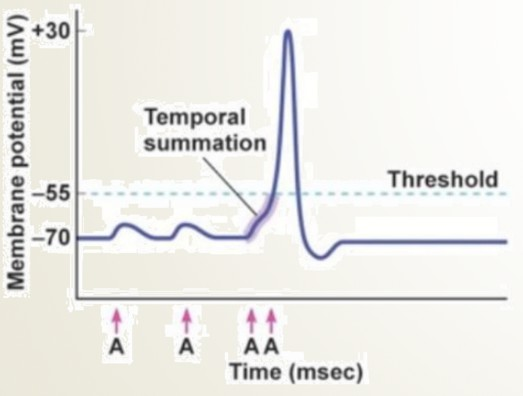
\includegraphics[width=0.80\textwidth]{images/image61.jpeg}
\end{figure}

Il modello pensato da Lapicque ha due comportamenti diversi per la membrana:

\begin{itemize}
  \item comportamento \textbf{\textit{sotto}}\textbf{\textit{ }}\textbf{\textit{soglia}};
  \item comportamento \textbf{\textit{sopra}}\textbf{\textit{ }}\textbf{\textit{soglia}}.
\end{itemize}
Una volta che il potenziale d'azione viene generato, l'informazione non è contenuta nel suo andamento, ma nell'istante in cui avviene.

\begin{itemize}
  \item \textbf{COMPORTAMENTO SOTTO SOGLIA}
\end{itemize}
Per quanto riguarda il comportamento sotto soglia, si tiene in considerazione una semplificazione del circuito equivalente, andando a trascurare i termini con conduttanza-voltaggio dipendente (per piccole variazioni sotto soglia questa è una buona approssimazione).

\begin{figure}[H]
  \centering
  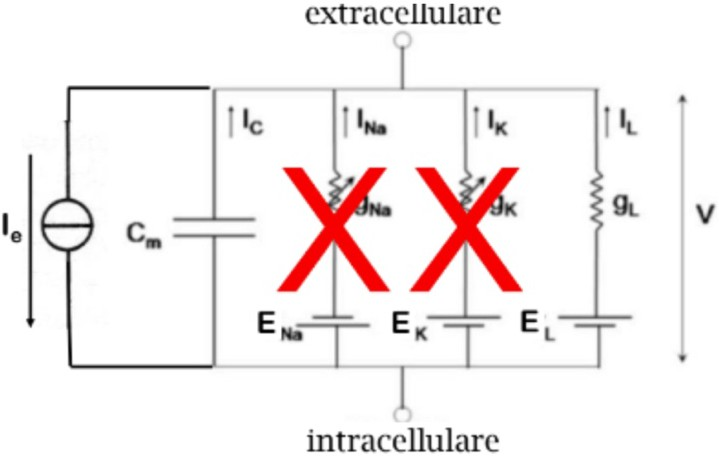
\includegraphics[width=0.80\textwidth]{images/image62.jpeg}
\end{figure}

In particolare, andremo a considerare solamente il ramo capacitivo (effetti capacitivi di membrana), il ramo resistivo (effetti sotto soglia) e il ramo con il generatore di corrente (stimolazione che simula le correnti
sinaptiche): si tratta quindi di un \textbf{\textit{circuito}}\textbf{\textit{ }}\textbf{\textit{RC}}.

\begin{itemize}
  \item \textbf{OSS 1: }eliminando il generatore di corrente la membrana è in equilibrio (potenziale di equilibrio).
  \item \textbf{OSS 2: }anche se considerassimo i canali del sodio e del potassio, sotto soglia
\end{itemize}
avrebbero una conduttanza pari a 0 $\rightarrow$ resistenza infinita $\rightarrow$ corrente nulla $\rightarrow$ eliminabili. Questo accade perché ci troviamo nel \textit{colle dell'assone}: ci fossimo trovati in una zona precedente, i canali sodio e potassio non ci sarebbero nemmeno stati. Quindi, questi canali in questa zona non si aprono se non viene raggiunta la soglia.

Analizziamo l'andamento delle tensioni e delle correnti.
Scriviamo innanzitutto un \textbf{bilancio delle correnti} (corrente iniettata = corrente di leakage + corrente capacitiva):

\[
I_e = \frac{V - E_L}{R_m} + C_m \frac{dV}{dt}
\]

Sostituiamo il tutto nell'equazione del condensatore (con capacità costante, V ed E variano) e normalizziamo per unità di area:

\[
C_m \frac{dV}{dt} = -\frac{V - E_L}{R_m} + I_e
\]

\textbf{N.B.} $R_L$ ($\Omega\,\text{m}^2$) è l'unico resistore del circuito e lo definiamo \textbf{resistenza di membrana} $R_m$ ($\Omega\,\text{m}^2$).

Moltiplichiamo a questo punto entrambi i membri per $R_m$:

\[
\tau_m \frac{dV}{dt} = E_L - V + R_m I_e
\]

dove: $\tau_m = R_m C_m = R_m \cdot C_m$ $\rightarrow$ \textit{costante di tempo del circuito RC}.

\textit{Resistenza totale di membrana} (unica R del circuito).

Quando viene iniettata corrente $I_e$, il potenziale di membrana varia con l'equazione scritta precedentemente. Se $I_e = 0$, il potenziale di membrana va esponenzialmente a $E_L$ (potenziale di riposo) con costante di tempo $\tau_m$:

\[
I_e = 0 \;\rightarrow\; \tau_m \frac{dV}{dt} = E_L - V
\]

Dividiamo tutto per $\tau_m$:

\[
\frac{dV}{dt} = \frac{E_L - V}{\tau_m}
\]

Questa è un'equazione differenziale lineare del primo ordine, la cui soluzione generale ha la forma:

\[
V(t) = E_L + (V_0 - E_L)\,e^{-t/\tau_m}
\]

dove: $V_0$ $\rightarrow$ \textit{valore iniziale del potenziale di membrana al tempo t=0}

\textbf{N.B. }se il potenziale di membrana è inizialmente diverso da 1/, in assenza di corrente esterna (*9 = 0) esso tende esponenzialmente a 1/.

\begin{itemize}
  \item \textbf{COMPORTAMENTO SOPRA SOGLIA}
\end{itemize}
Tutto ciò che avviene sopra soglia non può essere rappresentato dal circuito precedente, in quanto, tutto quello che Lapicque sapeva, era che il risultato fosse una \textbf{variazione di potenziale impulsivo }di una durata brevissima ( 1ms), ampiezza unitaria ( 1mV) e con verso depolarizzante (positivo) sempre uguale.

All'istante $t_0$ in cui il potenziale d'azione raggiunge il valore soglia $V_{\text{th}}$, viene imposto un

\begin{figure}[H]
  \centering
  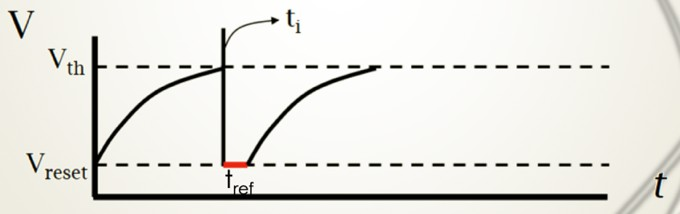
\includegraphics[width=0.80\textwidth]{images/image63.jpeg}
\end{figure}

potenziale d'azione B(( $-$ $t_0$) sulla membrana e il potenziale di membrana viene quindi posto al valore di riposo ':9?9) e mantenuto costante per il periodo di refrattarietà (:9@.

\begin{figure}[H]
  \centering
  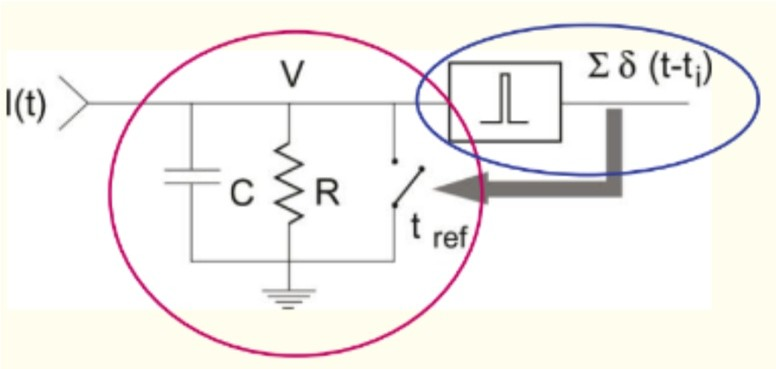
\includegraphics[width=0.80\textwidth]{images/image64.jpeg}
\end{figure}

\subsubsection{Circuito equivalente (modello ibrido)}

Per questo motivo, si è arrivati a costruire un circuito che \textbf{\textit{sotto soglia}}, si comporta come un \textbf{circuito RC}, mentre \textbf{\textit{sopra soglia}}, il circuito non funziona più ed entra in gioco un \textbf{generatore di impulsi }che, a richiesta, produce una \textit{delta di Dirac }con le stesse caratteristiche del potenziale d'azione: in questo modo si bypassa il problema di spiegare come si genera il potenziale d'azione.

\subsubsection{Potenziale di membrana}

Consideriamo un esempio con una corrente iniettata positiva, che simula la sinapsi eccitatoria. Prima di iniettarla tutto è \textbf{a riposo }(-70 mV), dopo di che, una volta iniettata, il potenziale di membrana diviene meno negativo, per cui si \textbf{\textit{depolarizza }}la
membrana. Se non si ha una corrente abbastanza elevata, non si raggiunge la soglia di -60 mV. Nel momento in cui si riduce la corrente iniettata e si riporta a zero, i meccanismi di equilibrio riportano la membrana a -70 mV.
\textbf{OSS: manca la refrattarietà}, infatti, quando il modello ``spara'' il potenziale d'azione, lo fa sempre alla stessa frequenza, ma non è così.

\subsubsection{Confronto con i dati sperimentali e limiti}

Nel modello integra-e-spara, quello che si osserva immediatamente è un \textbf{disallineamento tra dati computazionali e dati reali }su di un grafico in cui viene esplicitata il \textbf{\textit{legame lineare tra corrente }}CD \textbf{\textit{e la frequenza di scarica }}EABA\textbf{\textit{.}}
Questo accade a causa di alcuni meccanismi di memoria che fanno sì che, se si ripete la stimolazione sulla cellula vera, in
molti casi la risposta nel tempo cambia. Il modello RC, però, non tiene conto di ciò, al contrario della cellula.
Per i primi spike, il modello spiega bene i dati (retta e pallini neri), mentre per i successivi si discosta, perché non si tiene più conto dell'adattamento fisiologico della frequenza di spike che segue a stimolazioni continue.

\subsubsection{Refrattarieta' assoluta e relativa}

Come già anticipato, nel modello originale, viene totalmente ignorato il meccanismo di refrattarietà (sia assoluta che relativa). Ciò che si può fare per modellizzare gli intervalli di refrattarietà, è inserire una \textbf{conduttanza inibitoria }(che inibisce la generazione di un nuovo spike) \textit{a valori variabili nel tempo}. Questa conduttanza aumenterà subito dopo lo spike, rendendo il neurone meno eccitabile (\textbf{\textit{refrattarietà assoluta}}) e decrescerà esponenzialmente nel tempo, rendendo il neurone nuovamente eccitabile (\textbf{\textit{refrattarietà relativa}}). Quindi, quando il potenziale di soglia è raggiunto a breve distanza dal precedente, si inibisce un nuovo spike; quando la distanza temporale aumenta, si permette un nuovo spike ma con più difficoltà.
\textbf{N.B. }se non si inserisse questa conduttanza il tempo di reset e la frequenza di spiring sarebbero costanti, ma, come già anticipato, questo non è fisiologicamente possibile.
Risolviamo in questo modo il problema di fitting iniziale. La conduttanza inibitoria decade esponenzialmente dopo ogni spike:
\[
  g_{\text{inh}}(t) = g_{\text{inh},0}\,e^{-(t-t_0)/\tau_g}
\]
dove: $t_0$ $\rightarrow$ \textit{istante dell'ultimo spike}; \quad $\tau_g$ $\rightarrow$ \textit{tempo di decadimento della conduttanza inibitoria}.

L'equazione dell'integratore aggiornata diventa:
\[
  \tau_m \frac{dV}{dt} = -\,(V - V_{\text{rest}}) - r_m\,g_{\text{inh}}(t)\,(V - E_{\text{inh}})
\]
\begin{itemize}
  \item $V > V_{\text{th}}$:
\end{itemize}
\begin{figure}[H]
  \centering
  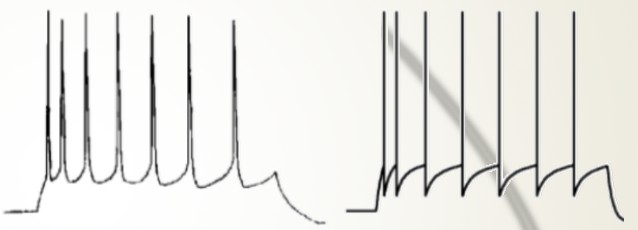
\includegraphics[width=0.80\textwidth]{images/image72.jpeg}
\end{figure}

\textit{Figura 1- Dati reali / dati computazionali}

Inserendo una conduttanza inibitoria variabile (come per la refrattarietà, ma con un tempo di recupero più lungo), si può modellizzare l'adattamento del neurone alla stimolazione ripetuta.

\begin{figure}[H]
  \centering
  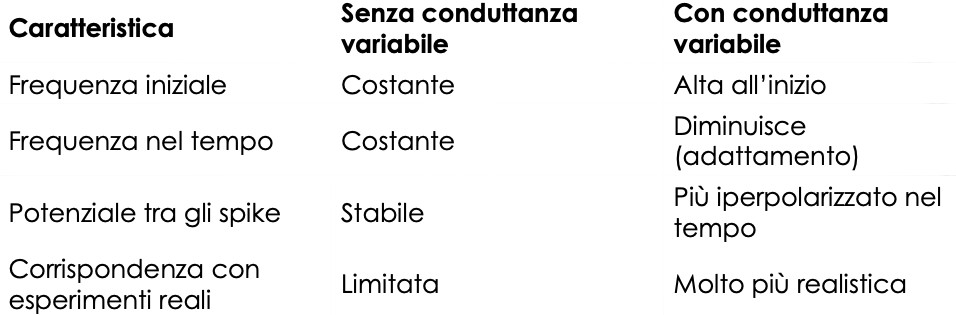
\includegraphics[width=0.80\textwidth]{images/image73.jpeg}
\end{figure}

\subsubsection{Conclusioni}

Il modello integra-e-spara, pur essendo molto semplice, riproduce abbastanza bene il comportamento del neurone dal punto di vista della generazione del potenziale d'azione. Sotto soglia funziona bene ma sopra soglia no, per questo motivo potrebbe essere utile complicare il modello con una conduttanza inibitoria per includere effetti di refrattarietà assoluta, refrattarietà relativa, adattamento della frequenza di spike. Il modello non tiene conto dei fenomeni sinaptici \textit{(come l'interazione tra neuroni, i neurotrasmettitori, ecc.) }e va bene se vogliamo includere il neurone in una rete più complessa.
Può essere utile arrivare ad un modello più fisiologico \textit{(modello di Hodgkin e Huxley).}


\section{Modello di Hodgkin e Huxley}

\subsubsection{Complessità nei modelli di neurone}

Il modello di Hodgkin e Huxley permette di descrivere dinamicamente la variazione di canali ionici (Na+, K+), considerando la dipendenza dal tempo dei meccanismi di propagazione del segnale. Il vantaggio di questo modello è che esso è molto fedele alla fisiologia anche se risulta più complesso rispetto al modello integra e spara, ma nonostante questo ha permesso di spiegare i meccanismi di \textbf{generazione }e di \textbf{propagazione del potenziale d'azione}. È stato ideato nel 1952, dai due scienziati, attraverso la combinazione di studi sperimentali, ipotesi teoriche, modellizzazione e data fitting. I loro studi si sono basati sull'\textbf{assone gigante di calamaro }(1 mm di diametro) in modo da poter svolgere misure più puntuali.
\subsubsection{Circuito equivalente di membrana}

\begin{figure}[H]
  \centering
  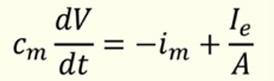
\includegraphics[width=0.80\textwidth]{images/image75.jpeg}
\end{figure}

Lo scopo di questo modello è spiegare i meccanismi alla base di generazione e propagazione del PA che si basano sulle variazioni della permeabilità di membrana. Partendo dal circuito sottosoglia, per studiare questo aspetto, bisogna andare a considerare i rami resistivi relativi ai canali ionici voltaggio dipendenti del Sodio e Potassio.
Questi due rami rappresentano i fenomeni che \textbf{variano nel tempo}, \textbf{al variare del potenziale di membrana }(V). (\textit{La variabilità è rappresentata dalla freccia sul resistore}). La variazione di conducibilità dei canali innesca \textbf{correnti ioniche di membrana}, producendo una variazione di V che a sua volta produce una \textbf{variazione della conducibilità}. Otteniamo un'equazione del circuito, applicando Kirchhoff, in cui la corrente \textit{Ic }viene espressa attraverso la derivata di V rispetto al tempo, queste variazioni inducono variazioni di \textit{im }(corrente che attraversa rami resistivi) mentre \textit{Ie }è la \textbf{corrente iniettata dall'esterno}. Per ogni ramo andiamo ad analizzare come si ottiene la conduttanza variabile da inserire poi nelle equazioni del circuito.
\textbf{Conduttanza del canale del K+ voltaggio dipendente}
Analizziamo il canale del potassio più semplice: presenta due stati (aperto o chiuso) controllati dal potenziale di membrana. Per quanto riguarda la conduttanza \textit{gk }andiamo a considerare più canali K+; infatti, sulla membrana cellulare è presente un numero abbastanza elevato di canali, che dipende dalla superficie di membrana e dal punto della membrana che si considera. Ciò che avviene è che le proteine cominciano a modificare la loro struttura via via che ci si avvicina alla soglia di apertura ma non lo fanno tutte allo stesso istante, per cui c'è un passaggio graduale dalla condizione in cui sono tutti chiusi a quella in cui sono tutti aperti, si ha una \textbf{transizione}.

\begin{figure}[H]
  \centering
  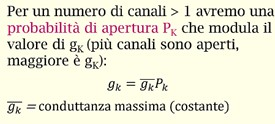
\includegraphics[width=0.80\textwidth]{images/image76.jpeg}
\end{figure}

Pertanto, la conducibilità si muove gradualmente tra un valore minimo (0 -- canali tutti chiusi) e un valore massimo (1- canali tutti aperti), gk può assumere un valore intermedio tra questi due estremi. Il valore massimo è costante, poiché una volta che si sono aperti tutti i canali la conduttanza è massima per cui il valore massimo di g è fisso e pari a gk. Il valore variabile della conduttanza si calcola moltiplicando il valore massimo di g per un numero compreso tra 0 e 1, che dice quanti canali sono aperti, questo valore è espresso tramite Pk che prende il nome di probabilità di apertura, che moltiplicata per il valore massimo di gk (calcolabile)
fornisce il \textit{gk intermedio in un determinato istante}. La probabilità di apertura dipende da V, ovvero dal potenziale di membrana. L'espressione per il Pk, trovata sperimentalmente dai due scienziati, è la seguente:
in cui:

\begin{figure}[H]
  \centering
  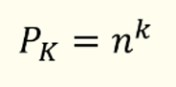
\includegraphics[width=0.80\textwidth]{images/image77.jpeg}
\end{figure}

\begin{itemize}
  \item \textbf{\textit{n }}è la variabile di attivazione (compresa tra 0 e 1) ed indica la probabilità che i canali siano aperti (modula il numero degli ioni che passano attraverso il canale quindi il valore della corrente che attraversa il canale, che a sua volta dipende dal potenziale di membrana)
  \item \textbf{\textit{k }}è un parametro da fittare sui dati (fattore di aggiustamento), sperimentalmente H \& H trovarono che \textbf{\textit{k}}\textbf{\textit{ }}\textbf{\textit{=}}\textbf{\textit{ }}\textbf{\textit{4}}\textbf{\textit{ }}( in seguito è stato dimostrato che k corrisponde al numero di componenti biologici che regolano il comportamento del canale).
\end{itemize}
A questo punto ci si può chiedere come varia $n$ nel tempo, in funzione di $V$. Sperimentalmente si è rivelato che la transizione da chiusi ad aperti avviene con una velocità voltaggio-dipendente indicata con $\alpha_n(V)$ (\textbf{tasso di apertura}); mentre la transizione da aperti a chiusi avviene con velocità $\beta_n(V)$ (\textbf{tasso di chiusura}). La velocità con cui cambia la \textbf{probabilità di apertura} dei canali è:
\[
\frac{dn}{dt} = \alpha_n(V)\,(1-n) - \beta_n(V)\,n
\]

quindi se n aumenta (canali aperti che aumentano) vuol dire che qualche canale che era chiuso si è aperto, questo aspetto viene messo in evidenza moltiplicando il tasso di apertura per la probabilità di canali chiusi  che  si  devono  ancora  aprire.

Diversamente n diminuisce quando i canali che erano precedentemente aperti si chiudono pertanto il tasso di chiusura è preceduto da un segno negativo e viene moltiplicato per la probabilità che i canali siano aperti (ovvero tutti i canali che devono ancora chiudersi). Il \textbf{tasso di apertura agisce sui canali chiusi}, mentre \textbf{quello di chiusura sui canali aperti}. Dato che $\alpha$n e $\beta$n dipendono da V, a seconda del valore del potenziale di membrana si avrà una certa velocità con cui i canali potassio si aprono e chiudono (dn/dt) e questo indica proprio come varia Pk nel tempo.
Possiamo ottenere un secondo modo di esprimere la variazione della \textbf{probabilità di apertura $n$} dividendo entrambi i membri per $\alpha_n(V) + \beta_n(V)$:
\[
\frac{dn}{dt} = \frac{n_\infty(V) - n}{\tau_n(V)}
\]

In questo modo introduciamo due nuove variabili: $\tau_n$, che ha le dimensioni di un tempo e indica quanto rapidamente $n$ varia nel tempo (\textbf{quanto tempo impiega per raggiungere il suo valore massimo}); e $n_\infty$, il valore della probabilità di apertura a regime (dopo un lungo tempo):
\[
n_\infty(V) = \frac{\alpha_n}{\alpha_n+\beta_n}, \qquad \tau_n(V) = \frac{1}{\alpha_n+\beta_n}
\]
Risolvendo l'equazione differenziale si ottiene l'andamento di $n$ nel tempo:
\[
n(t) = n_\infty + (n_0 - n_\infty)\,e^{-t/\tau_n}
\]
Ovvero, per $t\to\infty$, $n$ tende a $n_\infty$ con \textbf{andamento esponenziale}; la costante di tempo $\tau_n$ esprime la velocità di questo processo.

\begin{figure}[H]
  \centering
  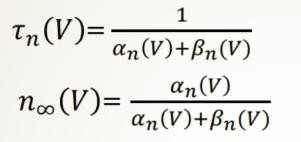
\includegraphics[width=0.80\textwidth]{images/image80.jpeg}
\end{figure}

\begin{figure}[H]
  \centering
  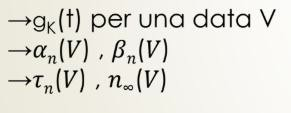
\includegraphics[width=0.80\textwidth]{images/image82.jpeg}
\end{figure}

Dal momento che possiamo misurare i valori di n$\infty$ e $\tau$n, possiamo andare a ricavare i valori di $\alpha$n(V) e $\beta$n(V) sperimentalmente. Per effettuare il fitting, occorre misurare l'ampiezza della corrente ionica di K+ che fluisce attraverso la membrana a diversi livelli del potenziale di membrana. Questa procedura rappresenta un problema dal momento che la corrente che fluisce attraverso la membrana fa cambiare il potenziale di membrana e di conseguenza la conduttanza della membrana (c'è una relazione mutua), quindi gk si modifica sia al variare del potenziale di membrana che nel tempo. La soluzione è quella di bloccare (clamp) il potenziale di membrana ad un valore costante nel tempo e registrare le correnti ioniche di membrana generate. In questo modo andiamo a studiare la dipendenza di gk(V, t) dal solo tempo (bloccando V). La funzione
fondamentale del circuito di blocco del voltaggio è quella \textbf{di impedire la mutua interazione fra apertura e chiusura dei canali ionici voltaggio-dipendenti (conduttanza) e potenziale di membrana}.


\subsubsection{Voltage clamp}

La tecnica del voltage clamp prevede un setting sperimentale composto da un circuito che possa mantenere il potenziale di membrana \textbf{Vm }ad un valore \textbf{costante}. Si procede andando ad inserire l'assone in un ambiente salino, poi si inserisce un \textbf{elettrodo di registrazione }all'interno, ed un secondo \textbf{elettrodo }esterno che costituisce la \textbf{referenza}, in questo modo è possibile misurare Vm istante per

\begin{figure}[H]
  \centering
  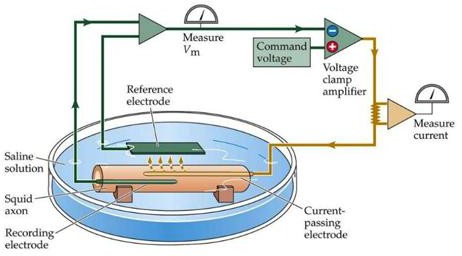
\includegraphics[width=0.80\textwidth]{images/image83.jpeg}
\end{figure}

istante tramite un oscilloscopio. Si avrà poi un operazionale che esegue il confronto tra la Vm misurata e la tensione di riferimento (command voltage). Se Vm è diverso dalla tensione di riferimento, un amplificatore di voltage clamp genera una corrente iniettata attraverso un secondo elettrodo (current-passing electrode), per riportare Vm al valore desiderato. La corrente necessaria per
mantenere Vm costante è esattamente uguale (ed opposta) alla \textbf{corrente ionica che passa attraverso i canali}. Quindi misurando questa corrente iniettata si ottiene la corrente ionica da analizzare. (Si misura la I nel tempo, ovvero la conduttanza della membrana gm).
Bloccando la tensione, i parametri introdotti diventano costanti. Si impongono, successivamente \textbf{variazioni di Vcmd }a gradino (per andare velocemente a regime n$\infty$) e si misura la corrente che fluisce attraverso la membrana, si ricavavano:

\begin{figure}[H]
  \centering
  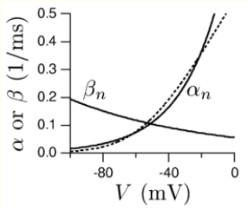
\includegraphics[width=0.80\textwidth]{images/image84.jpeg}
\end{figure}

In questo modo è possibile valutare l'andamento delle costanti, in funzione della tensione di membrana V e calcolare la conduttanza del canale in uno stato intermedio. Una volta ottenuti i parametri, possiamo ricavare n, da cui si ricava P, e infine la conduttanza variabile nel tempo. Le equazioni non sono semplici quindi solitamente si risolvono per via computazionale e non analitica.

\textbf{Conduttanza del canale del Na+ voltaggio dipendente}

\begin{figure}[H]
  \centering
  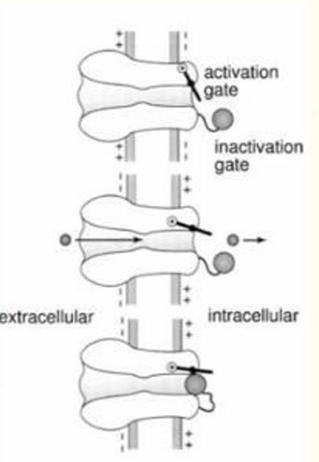
\includegraphics[width=0.80\textwidth]{images/image87.jpeg}
\end{figure}

Questo canale prevede 3 configurazioni: aperto, chiuso e inattivo. I canali sono aperti se non sono chiusi ne inattivi. Ciò che andiamo a descrivere sono le transizioni, quindi andiamo a considerare tanti canali presenti sulla membrana e non solo uno. Questo richiede una trattazione probabilistica. In questo caso la conduttanza, in un certo istante sarà data dal prodotto tra la conduttanza massima e la probabilità di apertura PNa che in questo caso sarà data da:
In cui:

\begin{itemize}
  \item \textbf{\textit{m}}\textbf{\textit{ }}è la probabilità che i canali \textbf{non siano chiusi }(ha lo stesso significato di n) ed è detta
\end{itemize}

\begin{itemize}
  \item \textbf{\textit{h}}\textbf{\textit{ }}è la probabilità che i canali \textbf{non siano inattivati }ed è detta \textbf{variabile di attivazione }(è uguale a 1 quando i canali sono tutti attivi, 0 quando sono tutti inattivi), anche questa variabile è elevata ad una costante che in questo caso è uguale a 1 quindi non compare;
  \item \textbf{\textit{k}}\textbf{\textit{ }}è una costante, H\&H trovarono che \textbf{\textit{k}}\textbf{\textit{ }}\textbf{\textit{=}}\textbf{\textit{ }}\textbf{\textit{3}}\textbf{\textit{ }}che corrisponde al numero di compartimenti mobili che si devono attivare affinché il canale sia aperto.
\end{itemize}
In questo modo \textbf{la conducibilità assume valori tra 0 e 1}. Durante la depolarizzazione si ha un aumento di m (i canali si aprono) e una lenta riduzione di h (alcuni canali cominciano ad essere inattivi), mentre quando la membrana si ri/iperpolarizza m si riduce (i canali sodio si chiudono) ed h aumenta (i canali si riportano alla condizione di equilibrio in cui sono attivabili).

\begin{figure}[H]
  \centering
  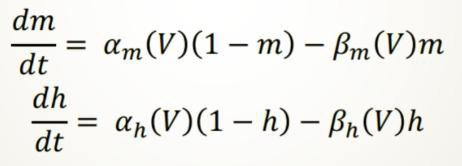
\includegraphics[width=0.80\textwidth]{images/image89.jpeg}
\end{figure}

Dato che si hanno due variabili, si ottengono due equazioni per analizzare la velocità di apertura/chiusura e attivazione/inattivazione dei canali:
\[
\frac{dm}{dt} = \alpha_m(V)\,(1-m) - \beta_m(V)\,m, \qquad
\frac{dh}{dt} = \alpha_h(V)\,(1-h) - \beta_h(V)\,h
\]

Oppure, in forma $\tau$/$x_\infty$:
\[
\frac{dm}{dt} = \frac{m_\infty(V) - m}{\tau_m(V)}, \qquad
\frac{dh}{dt} = \frac{h_\infty(V) - h}{\tau_h(V)}
\]

dove $\boldsymbol{\alpha_m}$ rappresenta il \textbf{tasso di apertura} dei canali chiusi, $\boldsymbol{\beta_m}$ il \textbf{tasso di chiusura} dei canali aperti; $\boldsymbol{\alpha_h}$ la \textbf{velocità con cui i canali smettono di essere inattivi} e $\boldsymbol{\beta_h}$ la \textbf{velocità di inattivazione}.
All'inizio della depolarizzazione m cresce e ciò corrisponde all'apertura dei canali sodio. Poco dopo, h diminuisce (alcuni canali sodio iniziano a inattivarsi), nel frattempo n aumenta in quanto i
canali potassio cominciano ad aprirsi per garantire la successiva fase di ripolarizzazione.

\begin{figure}[H]
  \centering
  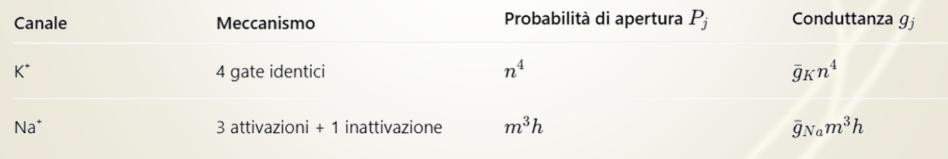
\includegraphics[width=0.80\textwidth]{images/image91.jpeg}
\end{figure}


\subsubsection{Modello di Hodgkin e Huxley}

A partire dal modello integra e spara andiamo ad aggiungere quanto ricavato dallo studio del canale sodio e del canale potassio, che caratterizzano la \textbf{generazione del potenziale d'azione}.

Nel circuito abbiamo due rami resistivi costituiti da un generatore di tensione e una resistenza variabile

\begin{figure}[H]
  \centering
  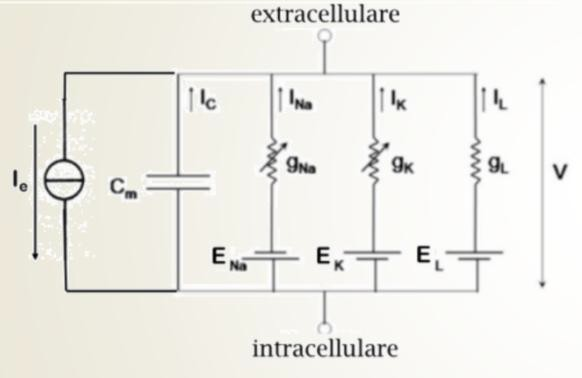
\includegraphics[width=0.80\textwidth]{images/image92.jpeg}
\end{figure}

nel tempo in funzione di V. il generatore rappresenta il potenziale di equilibrio elettrochimico della famiglia ionica che viene confrontato con V. Il verso dei due generatori che rappresentano il meccanismo delle due pompe (sodio e potassio) è invertito: le correnti di ioni Na+ e K+ hanno due effetti opposti, una è la depolarizzazione e una ripolarizzazione. L'intensità della corrente dipenderà dalla conduttanza variabile nel tempo gj(t,V).

\begin{figure}[H]
  \centering
  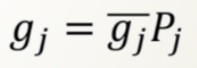
\includegraphics[width=0.80\textwidth]{images/image93.jpeg}
\end{figure}

Abbiamo ricavato che la conduttanza gj di un generico canale si ottiene moltiplicando la densità di canali della membrana, ovvero la conduttanza massima gj, per la frazione di canali che sono aperti in quel momento (probabilità Pj):

Possiamo riscrivere l'equazione delle correnti di equilibrio di membrana: al primo membro abbiamo le correnti capacitive, al secondo le correnti di membrana (\textit{im}) e la possibile corrente iniettata.

\begin{figure}[H]
  \centering
  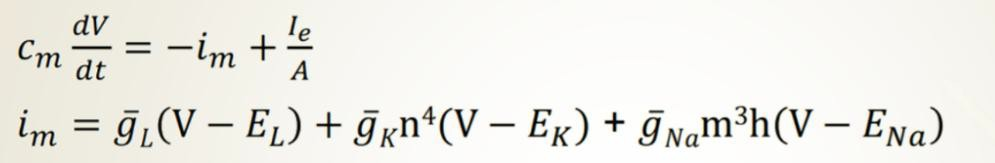
\includegraphics[width=0.80\textwidth]{images/image94.jpeg}
\end{figure}

La corrente di membrana \textit{im }contiene tutti i \textbf{meccanismi di trasporto di membrana }che si dividono in \textbf{costanti }(ramo di leakage, pompe sempre attive) e \textbf{variabili }(pompa sodio, pompa potassio). Per includere gli effetti sopra soglia dobbiamo includere due nuovi termini. Il primo termine rappresenta la \textit{corrente di ioni potassio }(data dalla conduttanza del canale che moltiplica la differenza di potenziale). Il secondo termine variabile è relativo alla \textit{corrente che scorre attraverso il canale ionico voltaggio dipendente del sodio}.

Mettendo tutto insieme otteniamo il modello di Hodgkin e Huxley:

\begin{figure}[H]
  \centering
  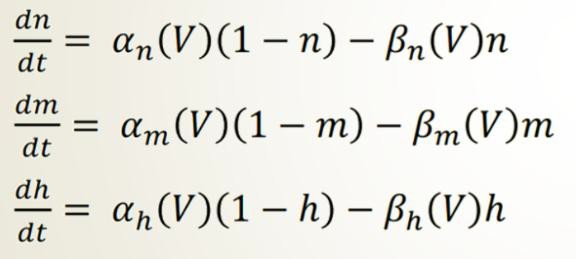
\includegraphics[width=0.80\textwidth]{images/image95.jpeg}
\end{figure}

modello circuitale

\begin{itemize}
  \item equazione del bilancio delle correnti + equazione della corrente di membrana
  \item andamento di n, m, h dato da 3 equazioni differenziali (che possono essere espresse anche tramite il valore limite e la costante di tempo)
\end{itemize}

\subsubsection{Dinamica di V ed im in funzione di n, m, h}

\begin{figure}[H]
  \centering
  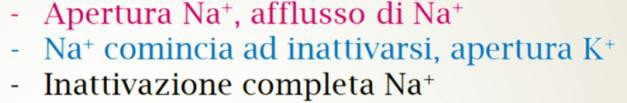
\includegraphics[width=0.80\textwidth]{images/image97.jpeg}
\end{figure}

Andiamo a vedere perché il canale Na+ ha 3 stadi e il K+ solo 2. riportiamo sulla stessa scala temporale il potenziale di membrana (V), il valore di \textit{im }e poi l'andamento delle tre variabili \textit{m}, \textit{h}, \textit{n}.

Esiste un potenziale di equilibrio (circa -70 mV) e una soglia di apertura dei canali sodio (circa -60 mV).

Vediamo che \textbf{all}'\textbf{equilibrio tutti i canali sono chiusi}. Dopodiché giunto uno stimolo \textbf{si supera la soglia di apertura del canale sodio}: questi si aprono e cominciano a far fluire ioni sodio creando una \textbf{corrente depolarizzante }negativa (\textit{im<0)}. Si verifica un aumento del numero di canali non chiusi (\textbf{m aumenta}).

\textbf{Al picco del potenziale d' azione }i canali del sodio sono tutti non chiusi e cominciano ad inattivarsi (+30mV). I canali non chiusi saranno in parte aperti e in parte inattivi (refrattarietà assoluta -- h scende). Nel frattempo, canali potassio si cominciano ad aprire in un transitorio (n aumenta). Aprendosi succede che nasce \textbf{una corrente ionica iperpolarizzante }(positiva). La corrente Na+ è maggiore e dura meno mentre quella K+ dura di più ed è più spalmata.

K+ tende a riportare il potenziale a riposo, ma in realtà abbiamo un'iperpolarizzazione dovuta alla

\textbf{lentezza dei canali K+ a chiudersi}.

I meccanismi del sodio sono cosiddetti \textbf{autoalimentanti}: appena si raggiunge il potenziale di soglia si crea un sistema a \textbf{feedback positivo}. (la corrente di depolarizzazione fa aprire i canali sodio, serve un blocco a questo meccanismo). Se non esistesse lo \textbf{stato di inattivazione del sodio}, la membrana non uscirebbe mai da questo circuito.

Nel caso degli ioni potassio, per innescare l'apertura dei canali abbiamo bisogno anche qui di una

\textbf{depolarizzazione}. Quando aumentano gli ioni potassio producono una corrente \textbf{iperpolarizzante }e

\begin{figure}[H]
  \centering
  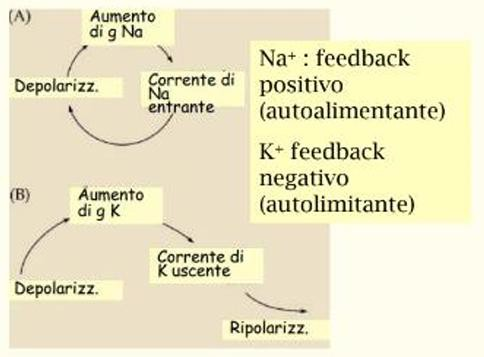
\includegraphics[width=0.80\textwidth]{images/image98.jpeg}
\end{figure}

quindi, anziché alimentare il processo, il processo si autoestingue. Si chiama processo autolimitante o a feedback negativo. Questo fa sì che nel caso del potassio non abbiamo bisogno del terzo stadio: l'apertura porta naturalmente alla chiusura. Al contrario negli ioni sodio non abbiamo un effetto limitante, ma la depolarizzazione produce depolarizzazione: se non esistesse l'inattivazione, il canale non tornerebbe mai alla situazione di chiusura.


\section{Modello delle correnti sinaptiche}


\subsubsection{Sinapsi chimica richiami}

Nella sinapsi chimica avvengono due eventi fondamentali: il \textbf{rilascio del neurotrasmettitor}e e la sua \textbf{azione sulla membrana postsinaptica}. Quando il potenziale d'azione raggiunge il bottone presinaptico, induce il rilascio del neurotrasmettitore nella fessura sinaptica. Le molecole rilasciate si legano ai recettori postsinaptici, provocando l'apertura dei canali ionici e generando una depolarizzazione (EPSP) o un'iperpolarizzazione (IPSP) della membrana. Nel modello questo processo serve a descrivere come un neurone integra i segnali provenienti dagli altri neuroni, introducendo una \textbf{corrente sinaptica }nelle equazioni. L'intensità di tale corrente dipende dalla presenza del neurotrasmettitore, dalla probabilità di apertura dei canali sinaptici e dal potenziale di membrana rispetto al gradiente elettrochimico. A differenza dei canali voltaggio-dipendenti per Na$^{+}$ e K$^{+}$, \textbf{questa conduttanza è chimicamente controllata}.


\subsubsection{Conduttanza sinaptica}

Nei precedenti esempi andavamo a considerare un solo neurone. In questo caso ne consideriamo 2:

\begin{itemize}
  \item \textbf{presinaptico }(rilascia neurotrasmettitori);
  \item \textbf{postsinaptico }(il neurotrasmettitore si lega ai recettori).
\end{itemize}
\begin{figure}[H]
  \centering
  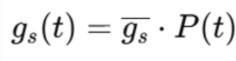
\includegraphics[width=0.80\textwidth]{images/image100.jpeg}
\end{figure}

Come per i canali voltaggio-dipendenti, ci serve la dipendenza della conduttanza dei canali postsinaptici dal tempo. Questa conduttanza dipende dal numero di canali aperti che può variare nel tempo. Avremo una conduttanza che è compresa tra 0 e la conduttanza massima relativa all'apertura di tutti i canali. La conduttanza variabile gs sarà espressa come prodotto tra la conduttanza massima (costante -- conduttanza del singolo canale moltiplicato per tutti i canali che ci sono) per la probabilità P che assume un valore tra 0 e 1, che pesa la quantità di canali aperti:

Cambia la \textit{P(t)}, ovvero cosa determina l'apertura dei canali (fenomeni presinaptici e fenomeni postsinaptici). P sarà data dal prodotto tra la \textbf{probabilità di rilascio del neurotrasmettitore \textit{Prel}}\textbf{\textit{ }}e la \textbf{probabilità di apertura sinaptica \textit{Ps}}. La probabilità di rilascio è la probabilità che si verifichino tutti i fenomeni presinaptici (arrivo del PA e rilascio del neurotrasmettitore). Mentre la probabilità di apertura sinaptica è la probabilità che il canale postsinaptico si apra, questo si apre solo se il neurotrasmettitore è stato rilasciato ovvero se è presente nella fessura sinaptica. P indica la \% di canali aperti dal neurotrasmettitore nel tempo. Non è un processo istantaneo, la conducibilità cambierà dunque nel tempo (e così la probabilità).

\begin{figure}[H]
  \centering
  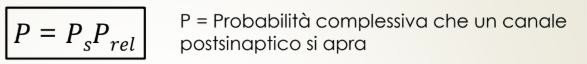
\includegraphics[width=0.80\textwidth]{images/image101.jpeg}
\end{figure}


\subsubsection{Probabilità di apertura sinaptica}

\begin{figure}[H]
  \centering
  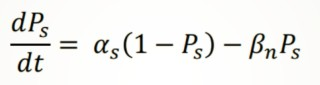
\includegraphics[width=0.80\textwidth]{images/image102.jpeg}
\end{figure}

La probabilità di apertura sinaptica (Ps) indica la probabilità che un canale postsinaptico si apra una volta rilasciato il neurotrasmettitore. Rappresenta quindi i meccanismi postsinaptici: legame del neurotrasmettitore ai recettori, velocità di apertura dei canali e dinamica di legame. Ps varia nel tempo in base al bilancio tra canali chiusi che si aprono (contributo positivo) e canali aperti che si chiudono (contributo negativo).

\begin{figure}[H]
  \centering
  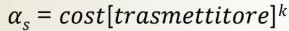
\includegraphics[width=0.80\textwidth]{images/image103.jpeg}
\end{figure}

I \textbf{tassi di apertura ($\alpha$) e chiusura ($\beta$) non dipendono dal potenziale di membrana}. \textbf{$\alpha$ }descrive la velocità di apertura dei canali chiusi ed è funzione della concentrazione di neurotrasmettitore: bassa concentrazione $\rightarrow$ legame lento; alta concentrazione $\rightarrow$ legame rapido. Se servono \textit{k }molecole per aprire un canale, questo valore compare come esponente nel termine di apertura. \textbf{$\beta$}, invece, è un tasso di chiusura costante, legato ai meccanismi che staccano il neurotrasmettitore dal recettore (degradazione, riassorbimento, diffusione).

\begin{figure}[H]
  \centering
  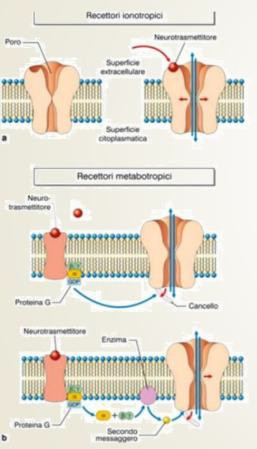
\includegraphics[width=0.80\textwidth]{images/image104.jpeg}
\end{figure}

Quando arriva un potenziale d'azione, la concentrazione di neurotrasmettitore aumenta rapidamente: $\alpha$ cresce, Ps sale. Poi, con la rimozione del neurotrasmettitore, $\alpha$ torna a zero e Ps decresce esponenzialmente. Diverse funzioni possono descrivere Ps in base al tipo di recettore coinvolto.

Questi possono essere di due tipi:

\begin{itemize}
  \item \textbf{\textit{Ionotropico:}}\textbf{\textit{ }}Il neurotrasmettitore si lega al canale e lo attiva direttamente. È più rapido (caratterizza riflessi)
  \item \textbf{\textit{Metabotropico:}}\textbf{\textit{ }}il neurotrasmettitore si lega ad un recettore distinto dal canale, il quale genera molecole dette \textit{messaggeri }che agiscono intracellularmente per attivare i canali. Si tratta di un meccanismo più lento che garantisce cambiamenti nel tempo che caratterizzano la plasticità e la flessibilità della cellula nervosa (memoria e apprendimento).
\end{itemize}
Per introdurre queste differenze si utilizzano \textbf{tre funzioni tipo o modelli principali}. Si vanno a graficare, sulla stessa scala temporale, il potenziale d'azione sul neurone presinaptico (spike), una corrente di membrana postsinaptica (EPSC) e il potenziale di membrana postsinaptica (EPSP). Per rappresentare la probabilità sinaptica, ovvero la probabilità che i canali siano aperti data la presenza del neurotrasmettitore, si usano:

\begin{itemize}
  \item \textit{Funzione esponenziale: }Si ha una costante di tempo pari all'inverso del tasso di chiusura. Questa equazione descrive una \textbf{apertura istantanea }(appena il neurotrasmettitore è presente), poi una \textbf{chiusura esponenziale }causata dall'aumento di $\beta$ che causa, in seguito all'apertura, i meccanismi che portano alla chiusura (riassorbimento, degradazione). Questa funzione rappresenta i canali a rapida apertura, per cui quando si hanno \textbf{sinapsi/recettori ionotropici}.
\end{itemize}
\begin{figure}[H]
  \centering
  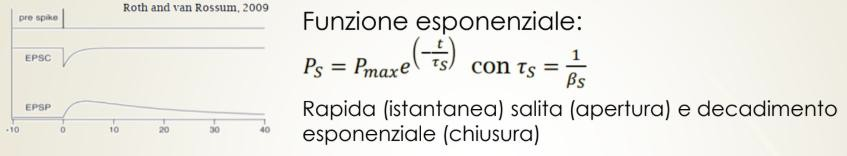
\includegraphics[width=0.80\textwidth]{images/image105.jpeg}
\end{figure}

\begin{itemize}
  \item \textit{Funzione alfa: }in questo caso la corrente raggiunge il picco seguendo un andamento esponenziale, il quale dipende dal tasso di apertura, questo modello rappresenta un tempo di \textbf{attivazione graduale}, il picco si raggiunge in corrispondenza di $\tau$s, poi la funzione decresce, la funzione modella sia la salita che la discesa con la stessa costante $\tau$s, utile per analizzare \textbf{sinapsi/recettori }con una risposta più lenta, per cui quelli di tipo \textbf{metabotropico}.
\end{itemize}
\begin{figure}[H]
  \centering
  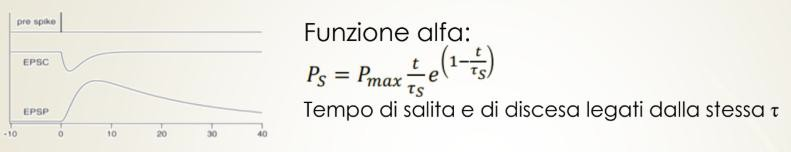
\includegraphics[width=0.80\textwidth]{images/image106.jpeg}
\end{figure}

\begin{itemize}
  \item \textit{Differenza tra due esponenziali: }Si tratta del caso più corretto in quanto tiene conto di una costante di tempo per la salita $\tau$1, e una per la fase di discesa $\tau$2; B rappresenta il fattore di normalizzazione per regolare il massimo della funzione; questa forma è molto flessibile e consente di rappresentare risposte sinaptiche che si attivano e disattivano con velocità diverse.
\end{itemize}
\begin{figure}[H]
  \centering
  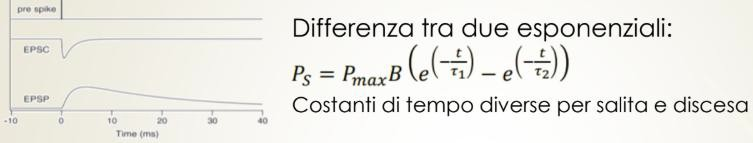
\includegraphics[width=0.80\textwidth]{images/image107.jpeg}
\end{figure}


\subsubsection{Probabilità di rilascio presinaptico}

Andiamo a vedere come varia la Probabilità di rilascio presinaptico \textbf{\textit{Prel}}. In condizioni normali, questa probabilità può considerarsi costante: un potenziale d'azione presinaptico causa il rilascio di neurotrasmettitore con probabilità fissa. Tuttavia, con \textbf{stimolazioni ripetute e ravvicinate}, Prel può cambiare nel tempo per effetto di due meccanismi principali:

\begin{figure}[H]
  \centering
  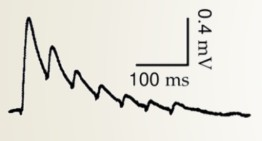
\includegraphics[width=0.80\textwidth]{images/image108.jpeg}
\end{figure}

Depressione sinaptica: Ogni volta che arriva uno stimolo, la probabilità di rilascio diminuisce. È un meccanismo che riduce la risposta sinaptica quando gli stimoli sono troppo ravvicinati, ad esempio perché le vescicole non hanno ancora fatto in tempo

a riformarsi per la successiva esocitosi del neurotrasmettitore. \textbf{\textit{f}}\textbf{\textit{D}}\textbf{\textit{ }}è un \textbf{fattore moltiplicativo }che regola quanto cala la probabilità, più è vicino a 0, più forte è la depressione. Nel grafico vediamo la risposta, ovvero che ESPS si indebolisce progressivamente.

\begin{figure}[H]
  \centering
  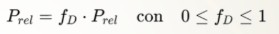
\includegraphics[width=0.80\textwidth]{images/image109.jpeg}
\end{figure}

\begin{figure}[H]
  \centering
  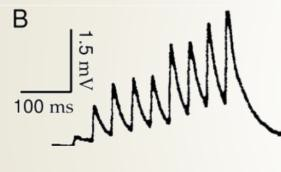
\includegraphics[width=0.80\textwidth]{images/image110.jpeg}
\end{figure}

Facilitazione sinaptica: in questo caso, la probabilità di rilascio aumenta ogni volta che arriva uno stimolo, perché la presenza continua di calcio residuo nel terminale presinaptico facilità il rilascio. fF è un fattore additivo che regola quanto cresce la probabilità, più è vicino a 1, più rapida è la facilitazione. Nel grafico vediamo l'aumento dell'ampiezza della risposta con stimoli successivi.


\subsubsection{Correnti sinaptiche}

Abbiamo detto che la conduttanza sinaptica dipende dal tempo e dalla probabilità che varia in base ai valori della probabilità di rilascio e apertura. Otteniamo così un valore di \textit{gs(t) }a cui corrisponde una \textbf{corrente sinaptica}, che quindi può essere inserita nel circuito. Si avrà un nuovo ramo che rappresenta l'effetto delle \textbf{correnti eccitatorie ed inibitorie}. Possiamo esprimere la \textbf{conduttanza sinaptica }come:

\begin{figure}[H]
  \centering
  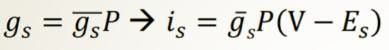
\includegraphics[width=0.80\textwidth]{images/image112.jpeg}
\end{figure}

dove Es rappresenta il potenziale di equilibrio elettrochimico dello ione relativo a quel tipo di canale

\begin{figure}[H]
  \centering
  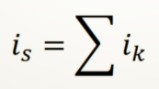
\includegraphics[width=0.80\textwidth]{images/image113.jpeg}
\end{figure}

Per k sinapsi si sommano le correnti, per comodità:

Quindi la corrente totale può essere scomposta in \textbf{due contributi}:

\begin{figure}[H]
  \centering
  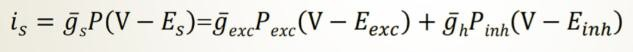
\includegraphics[width=0.80\textwidth]{images/image114.jpeg}
\end{figure}

\begin{itemize}
  \item \textbf{eccitatoria }(es. glutammato): tende a depolarizzare la membrana (cioè, aumentare V)
  \item \textbf{inibitoria }(es. GABA): tende a iperpolarizzare la membrana (cioè, diminuire V)
\end{itemize}
Queste due correnti possono essere aggiunte sia al modello integra e spara (in quanto sono attive anche sottosoglia) che al modello di Hodgkin e Huxley. In questo modello non abbiamo bisogno di correnti iniettate perché lo stimolo è generato dalle correnti sinaptiche.

\begin{figure}[H]
  \centering
  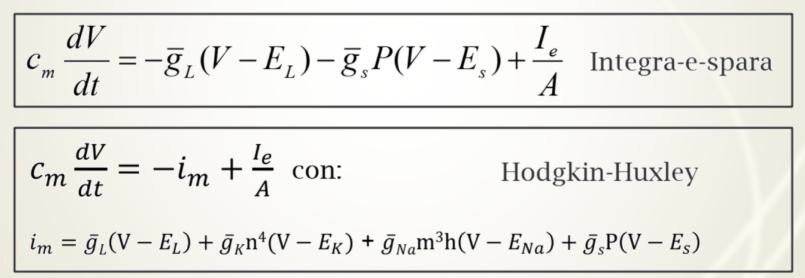
\includegraphics[width=0.80\textwidth]{images/image115.jpeg}
\end{figure}

\chapter{Modelli multicompartimentali della membrana neuronale}

\section{Modello di propagazione intracellulare}

Finora abbiamo ignorato la \textbf{dimensione spaziale}, scelta accettabile per descrivere i meccanismi di base (sinapsi, potenziale d’azione, sommazione temporale). Tuttavia, non è sufficiente quando si vogliono spiegare fenomeni come sommazione spaziale, propagazione lungo la membrana e conduzione del potenziale d’azione.

Anche se la struttura neuronale reale è tridimensionale e complessa, dendriti e assone possono essere \textbf{approssimati come cilindri}, o come combinazioni di cilindri $\Rightarrow$ questo permette di ridurre il problema alla sola dimensione \textbf{longitudinale ($x$)}: il potenziale di membrana $V$ dipenderà quindi dal tempo $t$ e dalla posizione $x$.

\begin{figure}[H]
  \centering
  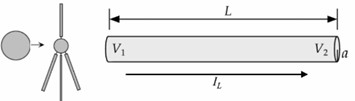
\includegraphics[width=0.80\textwidth]{images/image116.jpeg}
\end{figure}

\subsection{Propagazione passiva}

Il soma è rappresentato come un cilindro singolo, mentre l’albero dendritico come una serie di cilindri collegati.
Se in un punto della membrana si genera una variazione del potenziale ($V_1$), questa si ripercuote anche nelle zone vicine ($V_2$) per la propagazione passiva.

La depolarizzazione locale crea un gradiente di cariche all’interno del cilindro: gli ioni si spostano lungo questo gradiente generando correnti intracellulari longitudinali che modificano il potenziale nei punti vicini. Durante questo movimento, la corrente incontra una \textbf{resistenza longitudinale ($R_L$)}, che:
\begin{itemize}
  \item cresce con la lunghezza del cilindro;
  \item diminuisce con l’aumentare della sezione;
  \item è determinata da una resistenza specifica intracellulare $r_L$, tipicamente molto elevata (ordine dei k$\Omega\cdot$mm).
\end{itemize}

\begin{figure}[H]
  \centering
  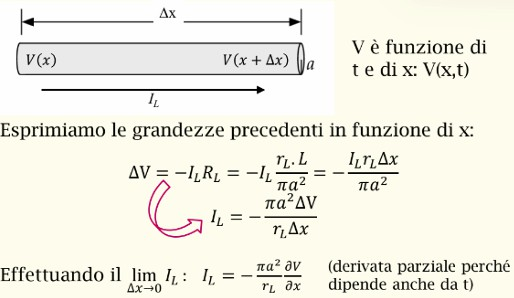
\includegraphics[width=0.80\textwidth]{images/image117.jpeg}
\end{figure}

\subsection{Teoria dei cavi}

Permette di descrivere il potenziale di membrana come funzione del tempo $t$ e della posizione $x$ lungo un cilindro che rappresenta un tratto di dendrite o assone. Questa teoria nasce dall’\textbf{analogia tra un neurone e un cavo elettrico}, adattata poi alle caratteristiche specifiche della membrana cellulare.

Considerando un piccolo segmento di cilindro di lunghezza $\Delta x$, si analizza la differenza di potenziale tra i suoi estremi, $V(x)$ e $V(x+\Delta x)$; questa è legata alla corrente longitudinale e alla resistenza interna. Facendo tendere $\Delta x$ a zero, la variazione $\Delta V/\Delta x$ diventa la derivata parziale di $V$ rispetto a $x$.

\begin{figure}[H]
  \centering
  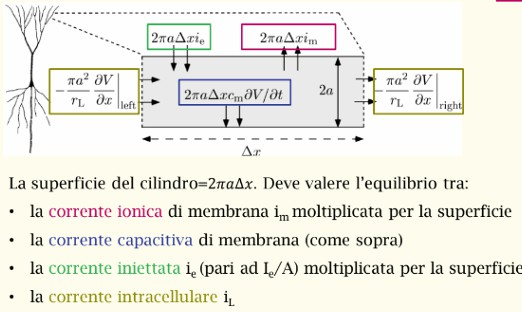
\includegraphics[width=0.80\textwidth]{images/image118.jpeg}
\end{figure}

Su un segmento infinitesimo agiscono tutte le correnti note del modello elettrico della membrana che devono rispettare il bilancio di corrente $\Rightarrow$ quello che entra nel cavo = quello che esce $\Rightarrow$ la loro somma deve essere nulla.
$$2\pi a \Delta x c_m \frac{\partial V}{\partial t} = \left. \left( \frac{\pi a^2}{r_L} \frac{\partial V}{\partial x} \right) \right|_+ - \left. \left( \frac{\pi a^2}{r_L} \frac{\partial V}{\partial x} \right) \right|_- - 2\pi a \Delta x i_m + 2\pi a \Delta x i_e$$
Dividendo tutto per la superficie laterale e semplificando si ottiene:
$$c_m \frac{\partial V}{\partial t} = \frac{1}{2\pi a \Delta x} \left[ \left. \left( \frac{\pi a^2}{r_L} \frac{\partial V}{\partial x} \right) \right|_+ - \left. \left( \frac{\pi a^2}{r_L} \frac{\partial V}{\partial x} \right) \right|_- \right] - (i_m - i_e)$$
Dividendo l’equazione per la superficie del cilindro ($2\pi a\Delta x$) e facendo tendere $\Delta x$ a zero, si ottiene l’\textbf{equazione dei telegrafisti}, che descrive come $V$ varia nel tempo e nello spazio (se la sezione non varia rispetto ad $x$ si può semplificare).
Per risolverla servono condizioni al contorno:
\begin{itemize}
  \item Il potenziale $V$ deve essere continuo per assicurare la continuità fisica del modello;
  \item Conservazione della carica o corrente nei nodi (leggi di Kirchhoff) per assicurare la corretta propagazione del segnale;
  \item Per avere coerenza elettrica, oltre che nei nodi, anche alle estremità ci sono diverse possibili condizioni, ma la più semplice è imporre la corrente di uscita nulla.
\end{itemize}


Poiché l’equazione completa è molto difficile da risolvere contenendo tutti i meccanismi di membrana, si \textbf{separano i processi di propagazione passiva da quelli di generazione del potenziale d’azione}. 

$$\text{se } V(t) < V_{th} : c_m \frac{dV}{dt} = -\bar{g}_L(V - E_L) + \frac{I_e}{A}$$
$$-\bar{g}_L(V - E_L) = -(V - V_{rest})/r_m$$

Per la propagazione passiva si usa il modello integra-e-spara in versione sotto soglia $\Rightarrow$ si possono trascurare i canali voltaggio-dipendenti e le correnti sinaptiche. La corrente di membrana è descritta come un semplice ramo resistivo.
$$c_m \frac{\partial V}{\partial t} = \frac{a}{2r_L} \frac{\partial^2 V}{\partial x^2} - (V - V_{rest})/r_m + i_e$$

La versione semplificata dell’equazione dei cavi è quindi adatta per descrivere la propagazione passiva, ma non la propagazione attiva del potenziale d’azione, per la quale servono modelli più complessi (multi-compartimentali).

\subsubsection{La Costante di Spazio ($\lambda$)}
Dalla risoluzione dell’equazione dei telegrafisti per la propagazione passiva in stato stazionario, emerge un parametro fondamentale: la \textbf{costante di spazio $\lambda$}, definita come:
\[ \lambda = \sqrt{\frac{r_m}{r_L}} \]
dove $r_m$ è la resistenza specifica di membrana e $r_L$ è la resistenza longitudinale interna. 
$\lambda$ rappresenta la distanza alla quale l’ampiezza del potenziale decade al 37\% (ovvero di un fattore $1/e$) del suo valore iniziale. La guaina mielinica, aumentando enormemente la resistenza di membrana $r_m$, fa aumentare drasticamente $\lambda$. Questo permette alla depolarizzazione di viaggiare passivamente per lunghe distanze all’interno dell’assone senza disperdersi, raggiungendo il nodo di Ranvier successivo con un’ampiezza ancora sufficiente per innescare un nuovo potenziale d’azione.


\section{Modello multi-compartimentale di propagazione del potenziale d’azione}

\subsection{Modelli multi-compartimentali}

Si spezza il modello in tanti compartimenti, spostando la dimensione spaziale dalla variabile $x$ alla numerazione dei singoli compartimenti $\Rightarrow$ ogni compartimento deve essere abbastanza piccolo da far sì che le variazioni spaziali di potenziale al suo interno siano trascurabili $\Rightarrow$ si approssima il potenziale continuo $V(x, t)$ in ogni compartimento (che però può variare da un compartimento all’altro).

\begin{figure}[H]
  \centering
  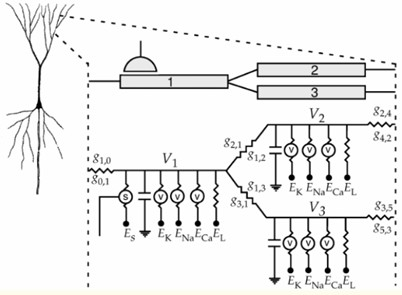
\includegraphics[width=0.80\textwidth]{images/image125.jpeg}
\end{figure}

Ogni compartimento si rappresenta con il modello circuitale di Hodgkin-Huxley: si inseriscono elementi circuitali a seconda di ciò che succede in un segmento di membrana.

\textbf{1) Compartimento “bottone sinaptico” (sinapsi):} ramo con le conduttanze sinaptiche ($S$) e canali ionici voltaggio-dipendenti $\Rightarrow$ rami potassio e sodio ($V$ indica resistenza variabile) + ramo effetti capacitivi e uno per leakage.

\textbf{2-3) Compartimenti intermedi:} non avendo sinapsi, hanno solo i canali ionici voltaggio-dipendenti con i relativi canali.

\begin{figure}[H]
  \centering
  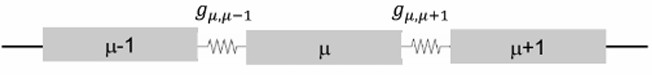
\includegraphics[width=0.80\textwidth]{images/image126.jpeg}
\end{figure}

Per tenere conto delle correnti intracellulari si inseriscono dei rami resistivi tra un compartimento e l'altro $\Rightarrow$ si separano i meccanismi di membrana (rappresentati nei compartimenti in parallelo) e i meccanismi di propagazione passiva (rappresentati dai rami resistivi longitudinali).

$$c_m \frac{dV_\mu}{dt} = -i_m^\mu + \frac{I_e^\mu}{A_\mu} + g_{\mu,\mu+1}(V_{\mu+1} - V_\mu) + g_{\mu,\mu-1}(V_{\mu-1} - V_\mu)$$

Quindi, per ciascun compartimento avremo la classica equazione che tiene conto delle correnti capacitive, delle correnti di membrana, delle correnti iniettate, e in aggiunta le correnti intracellulari; quest’ultime dipendono dalle conduttanze di raccordo e dalle differenze di potenziale tra il compartimento in esame e quelli adiacenti.

La \textbf{conduttanza di raccordo} rappresenta l’accoppiamento resistivo tra due compartimenti (il cilindro che li collega). Serve a modellizzare la caduta di potenziale che si verifica quando la depolarizzazione passa fisicamente da un compartimento al successivo.

La conduttanza specifica $g_{\mu,\mu+1}$ è calcolata per ogni tratto di raccordo (cilindrico) dividendo la $G_L$ per la superficie:

$$V_1 = V_\mu$$
$$V_2 = V_{\mu+1}$$
$$R_{L(\mu,\mu+1)} = \frac{r_L L}{\pi a^2}$$
$$G_{L(\mu,\mu+1)} = \frac{\pi a^2}{r_L L} \rightarrow g_{\mu,\mu+1} = \frac{\pi a^2}{r_L L} \frac{1}{2\pi a L} = \boxed{\frac{a}{2r_L L^2}}$$

Nell’equazione dei telegrafisti (modello continuo), si devono riportare le grandezze specifiche al caso fisico, in quanto le variazioni spaziali non sono trascurabili. Ma nel caso del modello multi-compartimentale si torna alle grandezze assolute $\Rightarrow$ la conduttanza di raccordo viene divisa per la superficie, ottenendo una formulazione più semplice da gestire.

Per semplificare la trattazione, consideriamo separatamente la propagazione continua da quella saltatoria.

\subsection{Propagazione continua del potenziale d’azione}

Nella propagazione continua, tipica degli \textbf{assoni non mielinizzati}, il potenziale d’azione si rigenera punto per punto lungo la membrana. Ogni tratto dell’assone si depolarizza e innesca la depolarizzazione del tratto successivo, mantenendo ampiezza e forma costanti.

Il modello compartimentale (es. a 100 compartimenti senza diramazioni) permette di:
\begin{figure}[H]
  \centering
  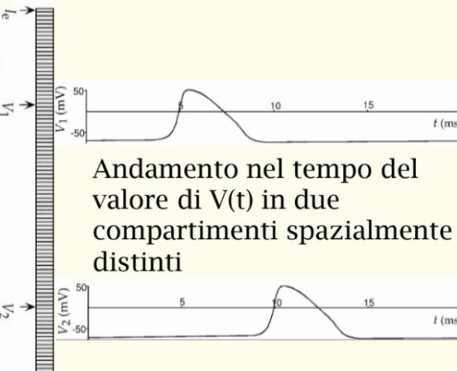
\includegraphics[width=0.80\textwidth]{images/image130.jpeg}
\end{figure}
rappresentare sia la componente temporale (osservando il singolo compartimento, dimensione continua), sia quella spaziale (spostandosi tra i vari compartimenti, dimensione discreta). Se la discretizzazione è fatta bene, non si perde molta informazione ed è più semplice rispetto all’equazione dei telegrafisti in forma continua.

Nel grafico a sinistra, si ha il modello=assone con tutti i compartimenti in serie e ognuno di essi con una $V$. Consideriamo solo 2 compartimenti ($V_1$ tra i primi, più vicino al soma; $V_2$ tra gli ultimi, più lontano).

\textbf{Per osservare la dimensione temporale}, ci concentriamo sul singolo compartimento. La corrente $I_e$ in alto è la corrente iniettata a $t = 0$ nel primo compartimento. Grazie alle conduttanze di raccordo, la perturbazione si propaga a quelli successivi in istanti di tempo diversi $\Rightarrow$ il modello emula ciò che succede nella cellula vera e sarà tanto più accurato quanto maggiore sarà la discretizzazione.

\textbf{Dal punto di vista spaziale}, per vedere come il potenziale viaggia lungo l’assone, riportiamo orizzontalmente il grafico. In questo caso non si considera tutto l’asse dei tempi, ma un istante specifico; cambiando istante, cambierà ciò che si vede nell’assone $\Rightarrow$ $V(x)$ è diversa istante per istante.
Scegliamo un istante di tempo fissato, per esempio \textbf{t = 9,75 ms} da quando si inietta la corrente.

\begin{figure}[H]
  \centering
  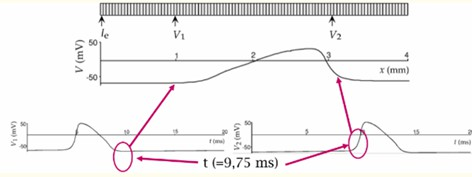
\includegraphics[width=0.80\textwidth]{images/image131.jpeg}
\end{figure}

\begin{itemize}
  \item Nel 1\textdegree{} compartimento non sarà presente il potenziale: la membrana è tornata allo stato di riposo poiché il potenziale d’azione dura molto meno di 10 ms.
  \item Nel tratto crescente la membrana si sta ripolarizzando: il potenziale è maggiore rispetto a quello di riposo perché è passato meno tempo da quando il potenziale è transitato in quel compartimento.
  \item Il picco corrisponde al compartimento in cui, in quell’istante, si ha il massimo del potenziale (+30 mV).
  \item Dopo il picco si trovano compartimenti in cui il potenziale d’azione non ha ancora raggiunto l’apice ma già risentono della depolarizzazione.
  \item Molto dopo si trovano compartimenti non ancora investiti dalla depolarizzazione, ancora in equilibrio.
\end{itemize}

\textbf{Attenzione:} i tratti orizzontali a sinistra rappresentano l’equilibrio a cui si è tornati dopo il passaggio del potenziale d’azione, mentre a destra l’equilibrio non è ancora stato perturbato.

Se si sceglie un istante di tempo maggiore, il grafico si sposterebbe verso destra, con un’area a riposo inferiore a sinistra $\Rightarrow$ l’unidirezionalità della propagazione è garantita dalla presenza nel modello H\&H dei canali del sodio voltaggio-dipendenti, che comportano la refrattarietà assoluta.

\subsection{Propagazione saltatoria del potenziale d’azione}
La propagazione saltatoria si verifica negli \textbf{assoni mielinizzati}, cioè fibre nervose ricoperte da una guaina mielinica formata da cellule (di Schwann o oligodendrociti) avvolte più volte attorno all’assone. Questo isolamento impedisce quasi totalmente il passaggio di corrente attraverso la membrana nei tratti mielinizzati.

\begin{figure}[H]
  \centering
  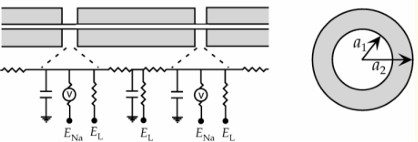
\includegraphics[width=0.80\textwidth]{images/image132.jpeg}
\end{figure}

La guaina non è continua: lascia delle piccole interruzioni chiamate \textbf{nodi di Ranvier}. Qui sono concentrati i canali ionici voltaggio-dipendenti, responsabili della generazione del potenziale d’azione. 
Anche in questo caso si usa un modello a compartimenti, ma con una differenza fondamentale:
\begin{itemize}
  \item \textbf{Nodi di Ranvier:} sono modellati con il circuito di Hodgkin-Huxley (contenente i canali voltaggio-dipendenti). Sono i punti in cui il potenziale d’azione viene realmente rigenerato.
  \item \textbf{Segmenti mielinizzati (internodi):} non hanno canali ionici $\Rightarrow$ non si usa né il modello H\&H né il modello “integra e spara”. Si equiparano i segmenti a zone con membrana spessa e senza canali ionici. Da un punto di vista circuitale sono dei condensatori in serie con una bassissima capacità. Gli effetti resistivi trasversali sono quasi infiniti (la mielina è un isolante), quindi si rappresentano con una resistenza di membrana molto elevata (conduttanza bassa).
\end{itemize}

I circuiti nodali sono poi raccordati da resistenze longitudinali che rappresentano la propagazione passiva all’interno degli internodi mielinizzati. Volendo si può aggiungere al modello un ultimo tratto che rappresenta il bottone sinaptico.
$$\frac{c_m 2\pi a L d_m}{\Delta a}$$

Interpretando la guaina mielinica come una serie di cilindri concentrici di spessore infinitesimo $\Delta a$, la capacità e la resistenza equivalente del tratto mielinizzato dipendono dai raggi interno ($a_1$) ed esterno ($a_2$) della guaina:
\begin{itemize}
    \item \textbf{Capacità equivalente ($C_{eq}$):} diminuisce logaritmicamente all’aumentare dello spessore della mielina:
    \[ C_{eq} \propto \frac{1}{\ln(a_2/a_1)} \]
    \item \textbf{Resistenza equivalente ($R_{eq}$):} aumenta logaritmicamente all’aumentare dello spessore della mielina:
    \[ R_{eq} \propto \ln(a_2/a_1) \]
\end{itemize}
Di conseguenza, maggiore è lo spessore della mielina (maggiore differenza tra $a_2$ e $a_1$), maggiore sarà la resistenza opposta alla fuoriuscita degli ioni e minore sarà la capacità che la cellula deve “caricare” per variare il potenziale.

\textbf{Come avviene la propagazione?}

La corrente che nasce da un nodo attivo scorre passivamente lungo il tratto mielinizzato, senza dispersioni verso l’esterno, grazie alla grande resistenza trasversale e alla bassa capacità della mielina.
Quando la corrente raggiunge il nodo successivo:
\begin{itemize}
  \item la depolarizzazione supera la soglia;
  \item si aprono i canali del sodio;
  \item si genera un nuovo potenziale d’azione.
\end{itemize}
$\Rightarrow$ Il potenziale d’azione quindi “salta” da un nodo all’altro, da cui il nome \textbf{propagazione saltatoria}.

Grazie alla mielina:
\begin{itemize}
  \item la membrana da caricare è molto meno (bassa capacità $\rightarrow$ si carica in fretta);
  \item la corrente si disperde pochissimo (alta resistenza trasversale);
  \item la depolarizzazione si trasmette molto più lontano (aumento della costante di spazio $\lambda$) e più rapidamente.
\end{itemize}
$\Rightarrow$ La velocità di conduzione è enormemente maggiore rispetto alla propagazione continua delle fibre non mielinizzate. In altre parole: più mielina = isolamento migliore = conduzione più veloce.

\clearpage
\section{Schemi Riassuntivi}

\subsubsection{Schema riassuntivo: Propagazione Passiva}
\begin{table}[H]
\centering
\renewcommand{\arraystretch}{1.5}
\begin{tabularx}{\textwidth}{l X}
\toprule
\textbf{Caratteristica} & \textbf{Descrizione} \\
\midrule
Tipo di modello & Teoria dei cavi (modello continuo spaziotemporale sotto soglia) \\
Correnti considerate & Solo correnti lineari di perdita (no canali voltaggio-dipendenti) e correnti longitudinali \\
Legge fisica & Equazione dei telegrafisti (versione semplificata) \\
Equazione & $\displaystyle \lambda^2 \frac{\partial^2 V}{\partial x^2} = \tau_m \frac{\partial V}{\partial t} + (V - E_L)$ \\
Limiti & Descrive solo l’attenuazione elettrotonica (passiva); non spiega la rigenerazione attiva del segnale. \\
\bottomrule
\end{tabularx}
\end{table}

\subsubsection{Schema riassuntivo: Propagazione Continua}
\begin{table}[H]
\centering
\renewcommand{\arraystretch}{1.5}
\begin{tabularx}{\textwidth}{l X}
\toprule
\textbf{Caratteristica} & \textbf{Descrizione} \\
\midrule
Tipo di modello & Hodgkin-Huxley (HH) multicompartimentale \\
Correnti considerate & Include i canali voltaggio-dipendenti (Na$^+$, K$^+$) \\
Equazione & Equazioni differenziali non lineari con variabili dinamiche ($m, h, n$) \\
Risultato & Propagazione \textbf{attiva} e continua lungo tutto l’assone \\
Esempio & Assone non mielinizzato modellato con $N$ compartimenti in serie \\
Osservazione & Il potenziale si rigenera e si propaga invariato nel tempo e nello spazio. \\
\bottomrule
\end{tabularx}
\end{table}

\subsubsection{Schema riassuntivo: Propagazione Saltatoria}
\begin{table}[H]
\centering
\renewcommand{\arraystretch}{1.5}
\begin{tabularx}{\textwidth}{l X}
\toprule
\textbf{Caratteristica} & \textbf{Descrizione} \\
\midrule
Tipo di modello & Modello ibrido: HH nei nodi di Ranvier + propagazione passiva (cavo) nei tratti mielinizzati \\
Struttura dell’assone & Alternanza di segmenti isolati (mielina) e segmenti nudi (nodi di Ranvier) \\
Modello fisico & Guaina modellata come condensatori in \textbf{serie} tra cilindri concentrici \\
Vantaggi fisici & Diminuzione drastica della capacità equivalente ($C_{eq}$) e aumento della resistenza ($R_{eq}$) \\
Conduzione & Velocità di conduzione enormemente maggiore, minore dissipazione di energia \\
Unidirezionalità & Garantita dall’inattivazione dei canali Na$^+$ (stato $h$) nei nodi appena attivati \\
\bottomrule
\end{tabularx}
\end{table}

\chapter{Modelli di encoding e decoding neuronale}

\section{4a. Funzione di risposta neuronale e frequenza di scarica}

\textbf{4a. Funzione di risposta neuronale e frequenza di scarica}

\subsubsection{Introduzione}

Questo argomento rappresenta il primo dei due principali modelli analizzati nel corso. Andiamo a riassumere il comportamento della cellula come una funzione che rappresenta un semplice legame ingresso-uscita:

Nello schema a lato (detto a scatola nera) è rappresentato rispettivamente: nella scatola al centro un insieme di neuroni che si comportano allo stesso modo e che indichiamo con il termine \textit{Neural Spiking System }(in cui spiking sta per: produce potenziali d'azione);

a sinistra l'\textit{input }che qui è una particolare caratteristica di un particolare stimolo ovvero un'unica variabile che varia nel tempo estratta da uno stimolo (esogeno se proveniente dall'esterno e endogeno se dall'interno); a destra invece c'è l'\textit{output }rappresentato da un treno di potenziali d'azione anche detti \textbf{spike }raffigurati come impulsi e non curve poiché quello che ci interessa in questo momento non è l'andamento del potenziale, bensì l'istante in cui questo avviene.

Si può dire che l'encoding/decoding neuronale consiste nel: misurare e caratterizzare il legame tra le caratteristiche di uno stimolo e i potenziali d'azione prodotti dalla cellula in risposta a quello stimolo. Vediamoli più in dettaglio:

Per \textbf{ENCODING }NEURALE si intende lo studio della risposta neuronale provocata da uno stimolo per cui si ha che: [Risposta neuronale = f(stimolo)] in cui l'obiettivo è descrivere come i neuroni rispondono a tanti stimoli. In altre parole l'encoding è una codifica da segnale continuo (ciò che riceve in ingresso) a binario (una risposta chiara per l'organismo). Per \textbf{DECODING }NEURALE invece si intende lo studio dello stimolo a partire dalla risposta da esso provocata ovvero l'operazione inversa alla precedente: [Stimolo = $f$$-$1(risposta neuronale)]. Qui l'obiettivo è risalire allo stimolo una volta ottenuto il treno di spike quindi una volta misurati i potenziali d'azione.

IL PROBLEMA DEL LEGAME STIMOLO-RISPOSTA

Nella realtà l'attività di un neurone non è sempre identica di fronte allo stesso stimolo poiché l'input non dipende solo dallo specifico stimolo ma anche dallo stato generale del soggetto in esame e inoltre il neurone fa parte di una rete, per cui le variazioni che agiscono su altri neuroni possono comunque modificarne il comportamento portandomi a dover studiare l'interconnessione tra neuroni. Quindi il treno di spike che viene prodotto risulta complesso e tale complessità porta a trattare il problema non deterministicamente (stimolo-> risposta) ma probabilisticamente (probabilità che un neurone risponda in un certo modo dato uno stimolo).

TRENI DI IMPULSI E FREQUENZA DI SCARICA

La misura dell'output neuronale può essere intra o extra cellulare. In questa trattazione utilizzeremo misure extra-cellulari le quali registrano le variazioni di carica all'esterno della membrana e consentono di studiare la risposta di uno o più neuroni in vivo, in relazione agli stimoli. In tali misure, ciò che interessa non è l'ampiezza del segnale, ma gli istanti in cui avvengono i potenziali d'azione, i quali vanno a identificare gli spike.

Posso andare a rappresentare la sequenza di spike come:
\[
\rho(t) = \sum_{i=1}^{n} \delta(t - t_i)
\]
dove $n$ è il numero di spike, $t_i$ l'istante in cui l'$i$-esimo spike ha avuto luogo, $i=1,2,\ldots,n$ e $0 \leq t_i \leq T$ dove $T$ è la durata del trial (singola presentazione dello stimolo). $\rho(t)$, somma di delta di Dirac, è detta \textbf{funzione di risposta neuronale} e descrive \emph{quando} un neurone genera potenziali, non quanto grandi questi siano.

\subsubsection{Ipotesi della codifica in frequenza}

Secondo l'ipotesi della codifica in frequenza: l'informazione ricavata dall'output della cellula non è contenuta né nell'ampiezza né nell'istante dei potenziali d'azione, bensì nella \textbf{frequenza di scarica }(firing rate) con cui essi si verificano. Questa ipotesi ha senso poiché la frequenza influenza il cosiddetto fenomeno della \textit{sommazione temporale}, secondo cui potenziali d'azione ravvicinati nel tempo (alta frequenza) si sommano ovvero il secondo stimolo arriva prima che il precedente sia completamente decaduto e quindi la risposta post-sinaptica viene amplificata. Se gli stimoli invece arrivano distanziati nel tempo (bassa frequenza) la probabilità che i potenziali si sommino diminuisce.

\begin{figure}[H]
  \centering
  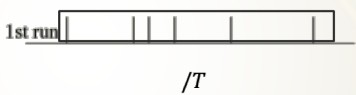
\includegraphics[width=0.80\textwidth]{images/image146.jpeg}
\end{figure}

\subsubsection{Frequenza di scarica}

Come abbiamo appena detto quindi la frequenza di scarica è la frequenza con cui un neurone invia potenziali d'azione ovvero con cui scarica uno stimolo elettrico, però è possibile illustrare 2 definizioni:

\textit{1° definizione:}

Data una risposta ottenuta come effetto diretto di uno stimolo, vado ad analizzare, per ogni trial, l'attività del neurone all'interno di una finestra temporale come in figura.

La frequenza di scarica si calcola come il rapporto tra \textit{n }numero di spike avvenuti nel trial e

\textit{T }durata di quest'ultimo che corrisponde ad integrare la funzione di risposta tra 0 e T.

La prima definizione, quindi, afferma che: la frequenza di scarica basata sul numero di spike è uguale alla media nel tempo dell'integrale della funzione di risposta neuronale effettuata sulla durata del trial. Es: se T=1s e n=6 -> r=6Hz

\textit{2° definizione:}

Uno svantaggio presente nella prima definizione è che non viene preservata l'informazione temporale e questo perché la frequenza viene calcolata sull'intero trial andando così a perdere risoluzione (non si tiene conto nelle variazioni nel trial). Per ovviare a questo, si prende un trial di lunghezza T come prima ma ora viene diviso per tanti $\Delta$t (con una finestratura arbitraria) così da effettuare la media non più sull'intero trial bensì su brevi

finestre temporali.

Anche qui però vi sono vantaggi e svantaggi perché: se $\Delta$t grande la risoluzione rimane bassa e se $\Delta$t piccolo si rischia di non avere nessuno spike all'interno della finestra.

Quest'ultimo problema si può risolvere effettuando registrazioni multi-trial e facendo la media lungo i trial. In figura abbiamo 3 trial e una finestra $\Delta$t e in base al numero di spike che si hanno in ogni trial nella finestra, è possibile esprimere la probabilità di avere uno spike in quest'ultima. L'ultimo grafico della figura (PSTH) è un istogramma che rappresenta la frequenza media di spike in funzione del tempo rispetto all'inizio di uno stimolo, calcolato su più trial. Quello che si osserva è che maggiore è il numero di spike e più la curva sale.

In conclusione, avere una registrazione di questo tipo permette di ridurre $\Delta$t e quindi di aumentare la risoluzione attribuendo alla frequenza di scarica un valore probabilistico. Si può anche effettuare la media sui trial e ottenere quindi una misura tempo variante di r(t).

n.b. anche la prima definizione può essere mediata sui vari trial

\subsubsection{Probabilità di scarica}

Sapendo che $r(t)\,\Delta t$ è il numero di spike tra t e $\Delta$t per ottenere il numero medio di spike su $\Delta$t maggiori basta integrare r(t) sull'intervallo di interesse. Ma se, come detto prima, $\Delta$t è piccolo, il numero di spike sarà sempre al massimo uno per trial e quindi $r(t)\,\Delta t$ è anche la frazione di trial in cui avviene uno spike nell'intervallo $\Delta$t intorno al tempo t. Per un numero molto grande di trial possiamo definire $r(t)\,\Delta t$ come la probabilità di scarica del neurone ovvero la probabilità che si generi un potenziale d'azione in un dato $\Delta t$.

\subsubsection{Limiti nel calcolo della frequenza di scarica $r(t)$}

Nella pratica, quanto appena detto, non avviene perché avrò un numero limitato di trial e quindi il calcolo della frequenza non sarà esatto bensì dovrà essere approssimato attraverso diversi approcci. Ora vedremo 4 approcci tutti su un singolo trial ma è possibile estenderlo al caso multi-trial semplicemente facendo la media lungo i trial.

\subsubsection{Calcolo di $r(t)$}

\textit{1° approccio}

Questo approccio consiste nel dividere il trial in finestre ed effettuare la media in ciascuna finestra. Nei grafici a lato, in cui si ha tempo in ascissa e frequenza in ordinata,

sono riportati rispettivamente: in A i potenziali d'azione in una finestra temporale pari a 3 secondi e in B invece la frequenza di scarica ottenuta andando a dividere in piccole finestre con dimensione a piacere; in questo caso le finestre sono da 100 ms quindi una volta visto quanti spike ci sono in 100 ms, come ad esempio 2, si fa la media e si ottiene la frequenza, pari a 20 Hz.

Il primo approccio presenta vari limiti ma il più importante è la bassa

risoluzione temporale poiché andando ad assumere che il numero di spike sia costante nelle finestre, qualcosa di rapido rischia di non essere rappresentativo. Quindi per risolvere dovrei andare a ridurre il $\Delta$t ma questo al contrario mi porta a

una diminuzione della risoluzione spettrale (al denominatore della formula avrei un valore più basso e quindi la frequenza risulterebbe un multiplo di 100 Hz invece che di 10 Hz). Bisogna quindi andare a scegliere un compromesso tra la risoluzione temporale e spettrale.

\textit{2° approccio}

\begin{figure}[H]
  \centering
  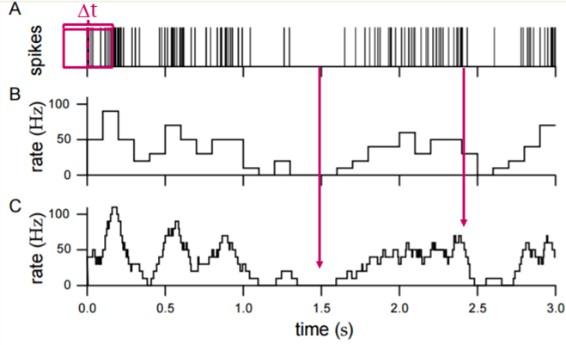
\includegraphics[width=0.80\textwidth]{images/image152.jpeg}
\end{figure}

Come nel primo approccio, anche qui si prende una finestra di ampiezza $\Delta$t ma invece di averne tante uguali disgiunte, se ne usa solo una e la si fa scorrere lungo il trial. Quello che si ottiene, rappresentato in figura C, è quindi una curva con una risoluzione temporale migliore (la frequenza cambia più velocemente) e il tutto senza perdere in termini di risoluzione spettrale (finestra più grande). Infatti vedendo il confronto con quello che abbiamo ottenuto prima è chiaro come i valori assunti sono gli stessi ma le variazioni nel tempo sono più veloci. Anche in questo caso però si stanno compiendo degli errori perché, quando si va a spostare la finestra, parte del contenuto sarà pari a quello della finestra precedente e quindi si andranno a

\begin{figure}[H]
  \centering
  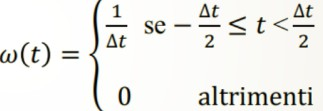
\includegraphics[width=0.80\textwidth]{images/image153.jpeg}
\end{figure}

prendere tutti gli spike della finestra precedente a meno di una piccola differenza.

Per risolvere questo bisognerebbe andare ad agire sul tipo finestra usata. Infatti in questo momento si sta utilizzando una funzione finestra mobile rettangolare $\omega$(t) con energia totale=1 che corrisponde ad uguagliare r(t) a una convoluzione tra $\rho$ e $\omega$:

\begin{figure}[H]
  \centering
  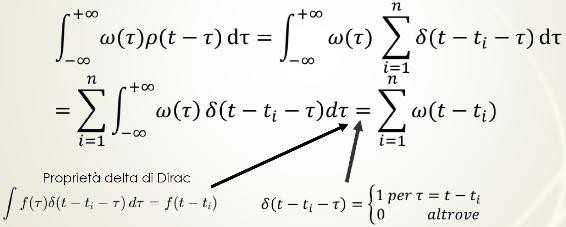
\includegraphics[width=0.80\textwidth]{images/image154.jpeg}
\end{figure}

n.b. le finestre risultano quindi correlate tra loro poiché i potenziali d'azione al suo interno vengono pesati allo stesso modo: questo significa che ogni spike che cade in una finestra contribuisce allo stesso modo al calcolo della frequenza e quindi non c'è differenza se avviene all'inizio, a metà o alla fine perché sarà sempre contato con lo stesso peso creando correlazione tra finestre vicine (ottengo risultati simili)

\textit{3° approccio}

\begin{figure}[H]
  \centering
  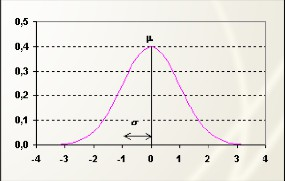
\includegraphics[width=0.80\textwidth]{images/image155.jpeg}
\end{figure}

Per ovviare al problema appena descritto può essere utile utilizzare una finestra non rettangolare, così da pesare meno i potenziali lontani da t e di più quelli vicino a t ricordando però che: il suo integrale nel tempo sia 1 e vada a 0 a breve distanza da t.

\begin{figure}[H]
  \centering
  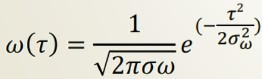
\includegraphics[width=0.80\textwidth]{images/image156.jpeg}
\end{figure}

Solitamente si prende una finestra Gaussiana a valor atteso nullo centrata nello 0: $\sigma$ ha lo stesso significato di $\Delta$t; $\sigma$$\omega$ regola la risoluzione temporale.

Quello che si ottiene in questo approccio non è più un andamento a

gradino dato dalla ripetizione nel conto degli spike, bensì una curva

\begin{figure}[H]
  \centering
  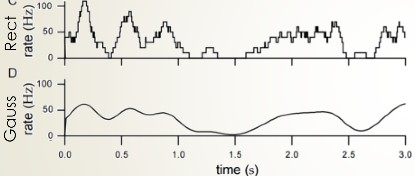
\includegraphics[width=0.80\textwidth]{images/image157.jpeg}
\end{figure}

molto liscia che riflette meglio l'influenza del neurone sulle cellule successive. Anche in questo caso però c'è qualcosa che non va e lo possiamo vedere confrontando le curve ottenute dai 3 approcci: tutte iniziano a salire anche prima che si verifichi lo spike e questo è dovuto al fatto che la finestra considera anche quello che avviene dopo quando nella realtà la risposta cellulare dipende solo da spike già avvenuti. Questo è dovuto al fatto che sto utilizzando finestre simmetriche rispetto allo zero, non casuali.

\begin{figure}[H]
  \centering
  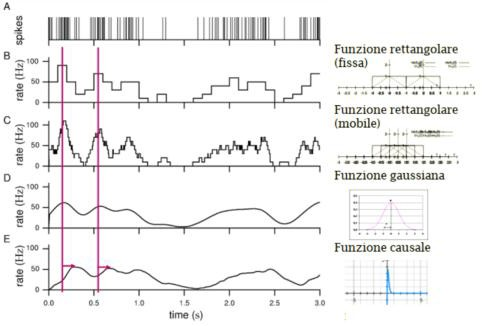
\includegraphics[width=0.80\textwidth]{images/image158.jpeg}
\end{figure}

\textit{4\textdegree{} approccio}

Per tenere conto di ciò si adotta un filtro CASUALE con $\omega$(t)=0 per t<0, di modo che nell'integrale di convoluzione vengano considerati solo gli spike passati. In questo modo la curva non presenta più anticipazioni ma i picchi corrispondenti a un aumento della densità di spike, appaiono più tardi riflettendo meglio la risposta reale della cellula.

Riassumendo:

\begin{figure}[H]
  \centering
  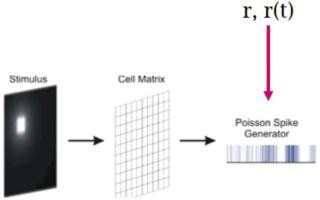
\includegraphics[width=0.80\textwidth]{images/image159.jpeg}
\end{figure}

\begin{figure}[H]
  \centering
  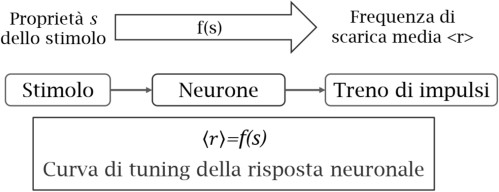
\includegraphics[width=0.80\textwidth]{images/image161.jpeg}
\end{figure}

\section{4b. Curve di Tuning}

\subsubsection{Introduzione}

Il concetto analizzato in questo capitolo è l'encoding e come abbiamo visto prima, un neurone o gruppo di neuroni ricevuto uno stimolo, produce una risposta, ossia una sequenza di potenziali d'azione. L'obiettivo però ora è quello di capire a cosa serve il neurone, quali stimoli riconosce e come reagisce. Per farlo, si sceglie una caratteristica quantificabile dello stimolo, che diventa l'input, mentre l'output è la frequenza

di scarica del neurone. Si considera quindi uno stimolo stazionario lungo il trial e si analizza la risposta r(t), che sarà costante e non tempo-variante come prima, media ottenuta da più trial.

La relazione tra la caratteristica dello stimolo \textbf{s }e la frequenza di scarica media

\textbf{<r> }è descritta da una funzione \textbf{f}, che prende il nome di \textbf{curva di tuning}.

Questa curva mostra come il neurone modula la sua risposta al variare di una

proprietà specifica dello stimolo ovvero come lo stimolo influenza la risposta neuronale.

\subsubsection{Costruzione di una curva di Tuning}

Costruire la curva equivale a risolvere il problema dell'encoding e per fare questo bisogna seguire 6 step:

\begin{itemize}
  \item Identificare la caratteristica dello stimolo s
  \item Far variare sistematicamente s effettuando diversi trial della stimolazione per ogni valore di s (fissando alcuni livelli di interesse, la s sarà costante su un trial ma diversa da trial a trial)
  \item Misurare ad ogni trial la risposta neuronale attraverso una registrazione extra-cellulare
  \item Calcolare la frequenza di scarica media lungo i trial <r> per ogni s
  \item Riportare i valori relativi alle coppie s/<r> su un grafico (ottenendo una curva sperimentale)
  \item Cercare una funzione matematica che approssimi i dati e al tempo stesso descriva il comportamento del neurone e permetta di fare previsioni anche per valori di s diversi da quelli testati.
\end{itemize}
\subsubsection{Stimolo costante, trial multipli}

Si può dimostrare che anche ripetendo più volte lo stesso stimolo, la risposta del neurone non è sempre uguale poiché il numero e la disposizione degli spike possono cambiare. Quindi per ottenere un risultato più stabile e rappresentativo, si calcola la frequenza media di scarica nei vari trial con un approccio probabilistico:
\[
\langle r \rangle = \frac{\langle n \rangle}{T} = \frac{1}{T}\int_0^T r(t)\,\mathrm{d}t
\]
dove $\langle n \rangle$ è il numero medio di spike su tutti i trial, $T$ la durata del trial, $r(t)$ la frequenza istantanea di scarica. Ovviamente più il numero dei trial è alto e più accurata sarà l'approssimazione della risposta reale.

\subsubsection{Esempi di curve di Tuning}

\textit{Esempio 1}

Consideriamo una stimolazione visiva: barra luminosa che viene ruotata e quindi cambia orientazione (stimolo esogeno). Il neurone della corteccia visiva primaria è specializzato nel riconoscere l'orientazione dello stimolo e quindi l'angolo rispetto all'orizziontale. Per ogni angolo si misura la risposta neuronale e si fa la media lungo i trial ottenendo così la frequenza di scarica media. Dopodichè si riportano sul grafico i punti che rappresentano le coppie angolo-frequenza di scarica (rispettivamente causa ed effetto) e si cerca una curva in

grado di interpolare questi punti. La curva in questione è una \textit{Gaussiana }che ha una espressione del tipo riportato a lato.

Dal grafico si osserva che: il neurone risponde solo a certe angolazioni mentre in altre è zero; esiste un angolo ottimale che provoca una risposta massima e man mano che ci si allontana da questo, la risposta diminuisce. Questo mi porta a dire che il neurone è tuned cioè è sintonizzato su una specifica orientazione.

Altri neuroni risponderanno ad angolazioni diverse così che l'insieme ricopra tutte le possibili orientazioni dello stimolo. La curva ottenuta ha un picco

centrale e una forma simmetrica, infatti angoli uguali ma con segno diverso producono la stessa frequenza di scarica, perciò conoscendo solo la frequenza non è possibile ricavare univocamente l'angolo. La curva è utile però a fare previsioni senza dover ripetere gli esperimenti.

\textit{Esempio 2}

\begin{figure}[H]
  \centering
  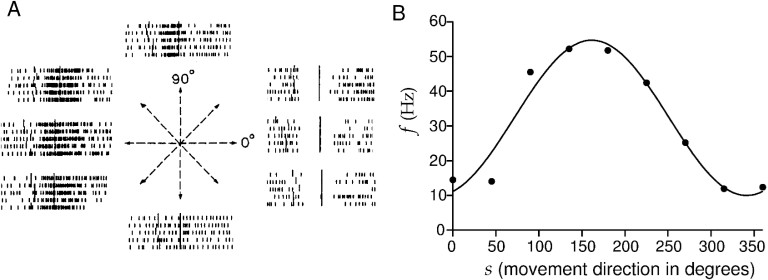
\includegraphics[width=0.80\textwidth]{images/image164.jpeg}
\end{figure}

In questo caso si studia uno stimolo endogeno, cioè un movimento volontario del braccio. La caratteristica analizzata è l'angolo del movimento (scelto dal soggetto ma comunque guidato attraverso oggetti verso cui muoversi) e le misure vengono fatte in vivo sui neuroni della corteccia motoria primaria. Per ogni angolo (0°-360°) il soggetto ripete il movimento per 5 volte, così da calcolare la media della frequenza di scarica del neurone per ogni angolo. I valori appena ricavati vengono poi rappresentati nel grafico che ha in ascissa

gli angoli e in ordinata la frequenza di scarica media. La curva che meglio approssima i dati sperimentali è la \textit{funzione coseno }(riportata a lato) ma dato che questa può dare anche valori negativi, a differenza della frequenza, si aggiunge un offset r0 per adattarla ai dati reali.

Dal grafico si osserva che: il punto più alto della curva s max indica la direzione preferita del neurone ovvero che provoca risposta massima r

max; il neurone risponde a tutti gli angoli anche se con intensità diversa; non è possibile ricavare in modo univoco l'angolo per lo stesso motivo di prima. Anche qui la curva descrive il comportamento del neurone e prevede le risposte di nuovi movimenti.

\textit{Esempio 3}

Nel primo esempio si è analizzato un neurone della corteccia occipitale sensibile all'orientazione dello stimolo visivo. In questo caso invece andremo ad analizzarne uno che risponde alla distanza di un oggetto rispetto all'osservatore.

Il cervello può calcolare la distanza grazie alla visione binoculare cioè l'uso di entrambi gli occhi: ogni occhio riceve l'immagine dell'oggetto in un punto leggermente diverso della retina e quando questo è perfettamente messo a fuoco, la sua immagine cade sulla fovea nel punto di fissazione F.

Se l'oggetto si avvicina -> l'immagine cade fuori dalla fovea formando un angolo con il piano del punto F negativo Se l'oggetto si allontana -> l'angolo è positivo

Se l'oggetto cade sul punto F -> l'angolo è 0

\begin{figure}[H]
  \centering
  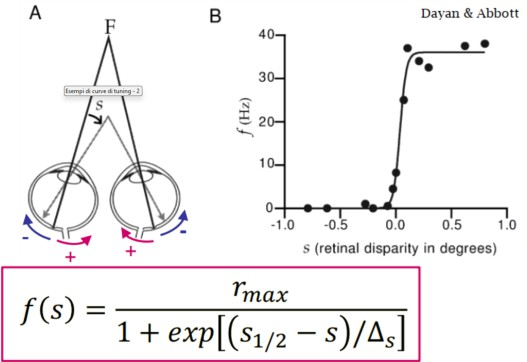
\includegraphics[width=0.80\textwidth]{images/image166.jpeg}
\end{figure}

L'angolo quindi mi dà informazioni sulla vininanza/lontananza dell'oggetto dagli occhi. Per i vari angoli e quindi per le diverse distanze degli oggetti si misurano le frequenze di scarica.

Dal grafico ottenuto si nota che: il neurone non risponde (frequenza = 0) per angoli negativi ovvero per oggetti molto vicini ma inizia a rispondere in modo crescente solo quando l'oggetto si avvicina al punto F (angolo 0); per oggetti lontani la frequenza si mantiene costante; si considera centro quello a cui otteniamo un valore pari a metà del massimo. Questo significa che il neurone è sensibile solo agli oggetti lontani rispetto ad F e non ha una risposta di tipo graduale bensì ha un salto molto netto:

lontano da F la frequenza è costante, l'unica differenza si ha tra la transizione max-min ovvero nell'intorno di F. Il neurone ha quindi una risposta binaria e per questo si parla di neurone far-tuned ovvero sintonizzato su distanze lontane.

Oltre a questi tipi di neuroni esisteranno ovviamente anche altri neuroni specializzati per oggetti più vicini così da coprire tutte le distanze visive.


\section{4c. Decoding neuronale}

Studio dello stimolo a partire dalla risposta provocata,si parte dagli effetti per risalire alle cause => stimolo=f\^{}-1(risposta neuronale)

Il problema si complica rispetto all'encoding poiché stimoli diversi producono una stessa risposta neuronale e bisogna adottare un approccio probabilistico per la complessità della rete di neuroni.

E per calcolare la probabilità dobbiamo prima descrivere il comportamento del neuroma in base allo stimolo => costruiamo un instrogramma

\begin{figure}[H]
  \centering
  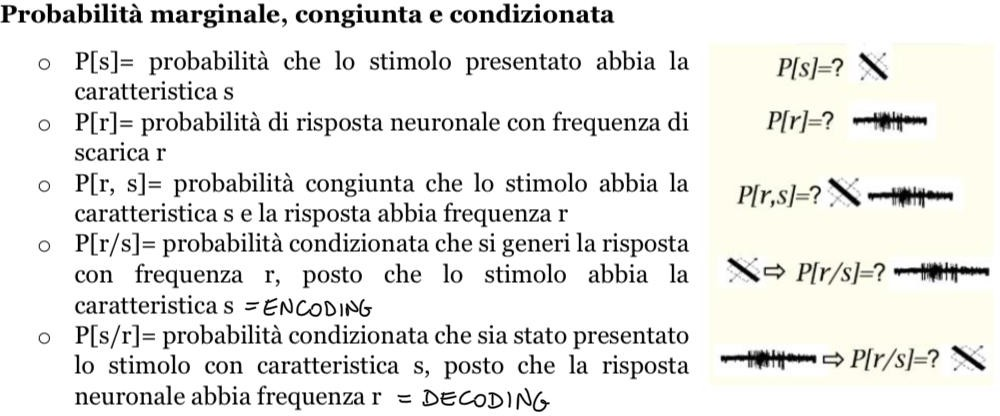
\includegraphics[width=0.80\textwidth]{images/image167.jpeg}
\end{figure}

\textbf{ESEMPIO DI ENCODING }=> considero un neurone della corteccia visiva effettuando misure invasive extracellulari sulla singola cellula in vivo

Il soggetto deve indicare la direzione di movimento dei punti sullo schermo (tra due direzioni opposte (+ -))

\begin{figure}[H]
  \centering
  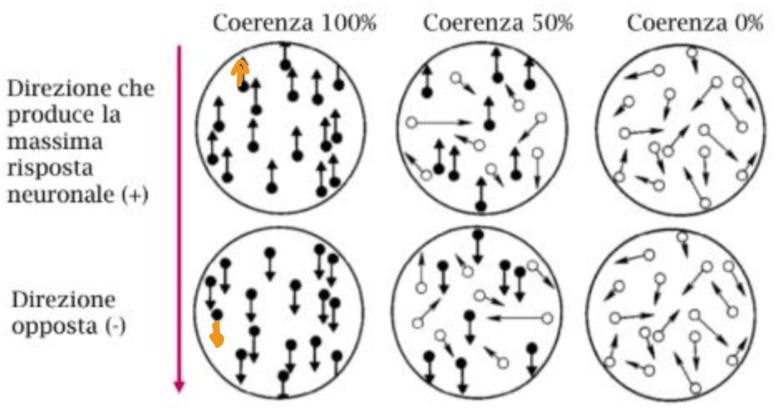
\includegraphics[width=0.80\textwidth]{images/image168.jpeg}
\end{figure}

Gli stimoli sono dei puntini in movimento di cui le frecce indicano la direzione (alto +, basso -) (la direzione che produce la massima risposte è +

Notiamo che i puntini neri si muovono coerentemente tra loro mentre quelli bianchi in maniera casuale,questo è indicato dal \textbf{livello di coerenza}=percentuale di punti che si muovono nella stessa direzione (100\% tutti stesso modo,0\% in maniera random)

=> direzione e coerenza sono i due fattori che posso manipolare nell'esperimento.

\textbf{DATI ACQUISITI }sono di 2 tipi:

\begin{itemize}
  \item NEURONALE=risposta neuronale e frequenza di scarica
  \item COMPORTAMENTALE=dato che si ottiene analizzando il comportamento del soggetto ovvero la funzione svolta e non l'attività cerebrale
\end{itemize}
\begin{figure}[H]
  \centering
  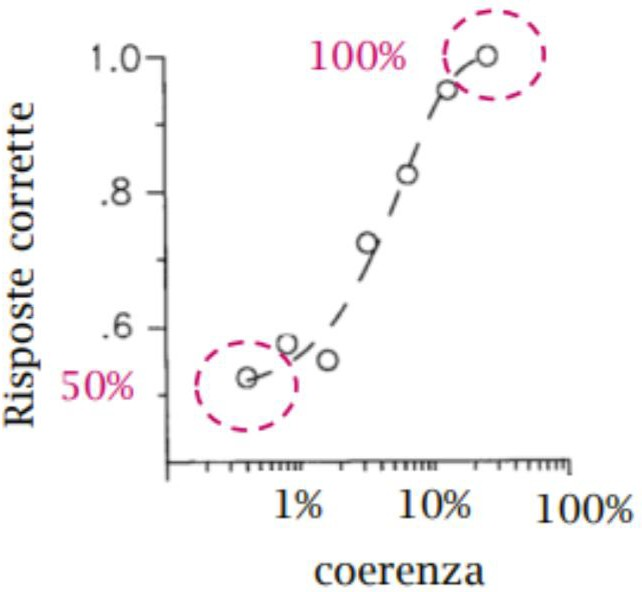
\includegraphics[width=0.80\textwidth]{images/image169.jpeg}
\end{figure}

X=livello di coerenza in scala logaritmica

Y=percentuali risposte corrette normalizzate a 1 (scala lineare)=(riconoscimento della direzione del movimento,dato comportamentale)

=>Ciò che si nota è che non vi sono valori inferiori a 0,5 (50\%) e si può affermare che il nostro cervello è molto bravo a riconoscere il movimento collettivo, poichè anche con un 90\% di rumore, è in grado di riconoscere la direzione corretta.

Va messa in relazione con il decoding neurale: l'obiettivo è capire se e quanto i neuroni registrati contengono informazioni che spiegano o predicono questo comportamento.


\subsubsection{Frequenza di scarica}

\begin{figure}[H]
  \centering
  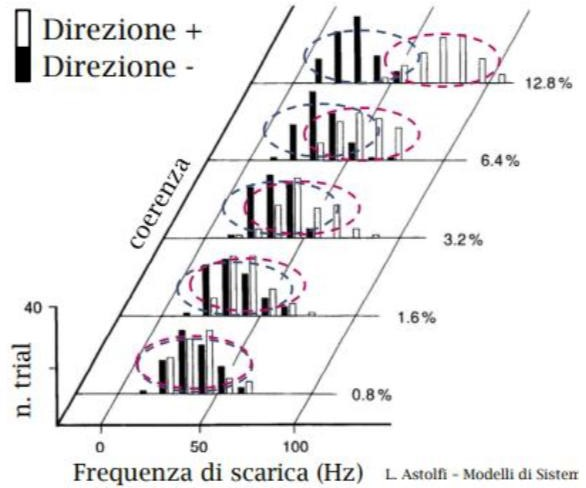
\includegraphics[width=0.80\textwidth]{images/image170.jpeg}
\end{figure}

Per calcolare la probabilità che, data una certa s, si abbia una certa r è necessaria una distribuzione empirica che si ottiene con un istogramma (numero di occorrenze) della frequenza di scarica r (X) calcolata per 60 trials (Y)

(Con infiniti trial, si otterrebbe la distribuzione esatta delle probabilità di risposta)

Combinazione dei due fattori:

\begin{itemize}
  \item Direzione del movimento [+ barre bianche; - barre nere]
  \item Livello di coerenza [0.8\%, 1.6\%,...,12.8\%]
\end{itemize}
Valori frequenti (es. 50 Hz) indicano risposte probabili, mentre valori mai osservati (es. 0 o 120 Hz) fanno dubitare che siano dovuti a quello stimolo.

Si costruiscono due istogrammi, uno per la direzione + e uno per la -- ,le due distribuzioni risultano diverse:

\begin{itemize}
  \item il picco per la direzione + è, ad esempio, a 50 Hz, mentre per la -- è a 30 Hz =>Il neurone è più sensibile direzione +
  \item si sovrappongono parzialmente: nella zona comune è difficile capire da quale direzione provenga lo stimolo; quando sono disgiunte, invece, la direzione si riconosce facilmente.
\end{itemize}
Ripetendo l'esperimento con diversi livelli di coerenza (cioè quanto i pallini si muovono in modo coordinato), si osserva che:

\begin{itemize}
  \item per la direzione -- la risposta del neurone resta sempre uguale (non è sensibile);
  \item per la direzione + la risposta aumenta con la coerenza dello stimolo $\rightarrow$ \textbf{ma}ggiore coerenza, maggiore risposta neuronale.
\end{itemize}
Per misurare quanto è facile distinguere le due direzioni si usa un \textbf{indice di discriminabilità}, che dipende:

\begin{figure}[H]
  \centering
  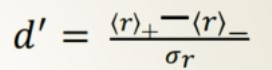
\includegraphics[width=0.80\textwidth]{images/image171.jpeg}
\end{figure}

dalla differenza tra le medie delle due distribuzioni (maggiore distanza $\rightarrow$ migliore discriminazione);

\begin{itemize}
  \item dalla \textbf{larghezza delle curve }(curve più strette $\rightarrow$ minore errore), assumiamo la deviazione standard uguale per entrambe
\end{itemize}
\textbf{CLASSIFICAZIONE A SOGLIA DELLA RISPOSTA}=metodo più semplice di decoding

si stabilisce un valore limite (\textbf{soglia z}) che separa le due distribuzioni di risposta (una per la direzione + e una per la direzione --).

\begin{itemize}
  \item Se la frequenza di scarica r $\geq$ z, si attribuisce la risposta alla direzione +.
  \item Se r < z, si attribuisce alla direzione --.
\end{itemize}
La soglia va scelta con attenzione: deve trovarsi \textbf{circa a metà tra le due distribuzioni}, per ridurre al minimo gli errori; la sua efficacia dipende sia dalla \textbf{scelta di z }(che possiamo controllare), sia dalla \textbf{forma delle distribuzioni }(che non possiamo controllare).

=>Una buona soglia consente di ottenere una classificazione accurata; se invece le distribuzioni sono troppo sovrapposte, anche la soglia migliore produrrà risultati meno precisi.

\textbf{VALUTAZIONE DELLA QUALITÀ DEL CLASSIFICATORE=}quanto bene il sistema distingue tra direzione +--si analizzano i possibili tipi di risposta:

\begin{figure}[H]
  \centering
  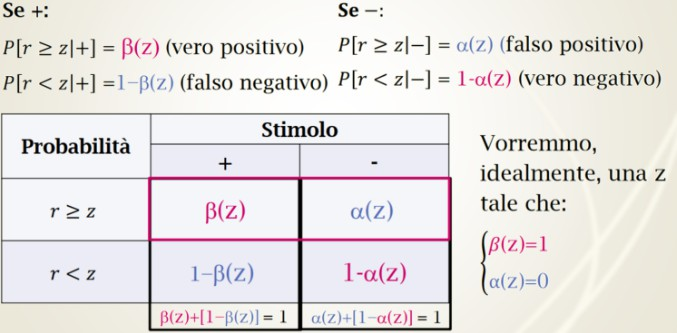
\includegraphics[width=0.80\textwidth]{images/image172.jpeg}
\end{figure}

Vero positivo ($\beta$(z)) $\rightarrow$ si riconosce correttamente uno stimolo positivo.

\begin{itemize}
  \item Falso positivo ($\alpha$(z)) $\rightarrow$ si indica come positivo uno stimolo che in realtà è negativo.
  \item Vero negativo (1$-$$\alpha$(z))
\end{itemize}
$\rightarrow$ si riconosce correttamente uno stimolo negativo.

\begin{itemize}
  \item Falso negativo (1$-$$\beta$(z))
\end{itemize}
$\rightarrow$ si indica come negativo uno stimolo che in realtà è positivo.

L'obiettivo ideale è eliminare gli errori (nessun falso positivo o falso negativo), ma spesso non è possibile: modificando la soglia z, si può ridurre un tipo di errore a scapito dell'altro.

Per questo si bilanciano sensibilità (capacità di riconoscere i veri positivi) e specificità (capacità di evitare falsi positivi), scegliendo la soglia ottimale che garantisce il miglior compromesso.

\begin{figure}[H]
  \centering
  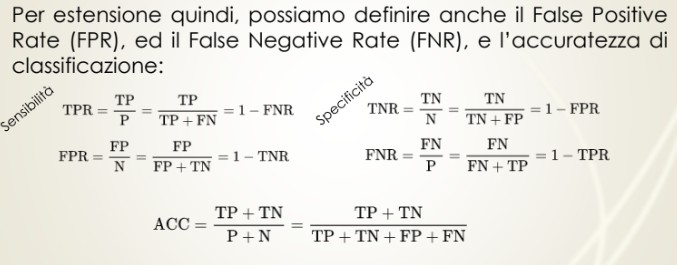
\includegraphics[width=0.80\textwidth]{images/image173.jpeg}
\end{figure}

I parametri $\alpha$ e $\beta$ dipendono da z: spostando la soglia cambiano i tassi di errore.

Inoltre, i quattro casi (VP, FP, VN, FN) non sono indipendenti: ad esempio, se aumentano i veri positivi, diminuiscono i falsi negativi, e la somma dei due deve sempre dare il totale dei casi=> i parametri sono correlati, e ne basta utilizzarne due.

Per rappresentare graficamente questo equilibrio e trovare la soglia migliore si utilizzano le curve ROC, che mostrano in modo immediato l'accuratezza del sistema.


\section{Teoria delle curve ROC}

Le curve ROC rappresentano graficamente la capacità di un \textbf{classificatore binario }di distinguere tra due classi, variando la soglia di decisione (threshold) per trovare il miglior equilibrio tra sensibilità e specificità.

\begin{figure}[H]
  \centering
  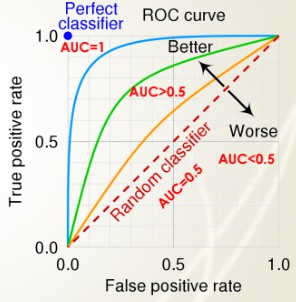
\includegraphics[width=0.80\textwidth]{images/image176.jpeg}
\end{figure}

Asse Y: TPR (True Positive Rate) = Sensibilità Asse X: FPR (False Positive Rate) = 1 - Specificità

=> è anche detta grafico sensibilità vs (1 - specificità).

Il \textbf{punto ideale }sul grafico è (0,1): rappresenta la classificazione perfetta (100\% sensibilità e 100\% specificità).

Una \textbf{classificazione casuale }produce invece una linea diagonale (da (0,0) a (1,1)), detta \textbf{linea di non discriminazione}.

\begin{itemize}
  \item Punti \textbf{sopra }la diagonale: buoni classificatori
  \item Punti \textbf{sotto }la diagonale: classificatori peggiori del caso
\end{itemize}
L'\textbf{area sotto la curva (AUC -- Area Under the Curve) }misura la capacità complessiva del classificatore di distinguere le due classi: rappresenta la probabilità che un'istanza positiva casuale sia classificata meglio di una negativa.

Un'AUC vicina a \textbf{1} indica prestazioni elevate, mentre un'AUC di \textbf{0.5 }corrisponde a un comportamento casuale.

\textbf{Determinazione della soglia ottimale }con due criteri principali:

\begin{itemize}
  \item Threshold in corrispondenza della distanza minima da [0,1];
  \item Threshold ad accuratezza più alta:
\end{itemize}

\subsubsection{Costruzione della curva ROC}

\begin{itemize}
  \item Costruire la matrice [y;d], dove y è la funzione discriminante (<r> neurone)(es output del neurone) e d è il vettore della classe corretta [0,0,0,\ldots{},1,1,1,\ldots{}].
  \item Ordinare i valori di y in ordine crescente.
  \item Calcolare, per ogni soglia y(i) con i=1:length(y): TP, TN, FP, FN, quindi TPR, FPR e Accuracy.
  \item Rappresentare TPR in funzione di FPR.
  \item Calcolare AUC = 1 - |trapz(TPR, FPR)|.
\end{itemize}

\subsubsection{Applicazione al decoding neurale}

\begin{figure}[H]
  \centering
  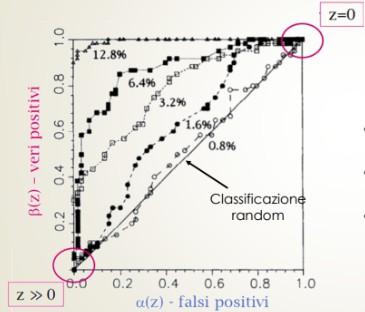
\includegraphics[width=0.80\textwidth]{images/image177.jpeg}
\end{figure}

Nel contesto del decoding neurale, le curve ROC sono utilizzate per valutare l'efficacia del decoder neurale nel distinguere tra due direzioni di movimento (+ e $-$).

Ogni punto della curva corrisponde a un valore di soglia \textit{z}, espresso come [$\alpha$(z),$\beta$(z)], e per ciascun \textbf{livello di coerenza }(es. 0.8\%, 12.8\%) si ottiene una curva distinta.

Gli estremi delle curve coincidono:

\begin{itemize}
  \item per z = 0 $\rightarrow$ a(z) = 1, b(z) = 1
  \item per z $\gg$ 0 $\rightarrow$ a(z) = 0, b(z) = 0
\end{itemize}
L'andamento della curva ROC riflette le prestazioni del classificatore:

\begin{itemize}
  \item una \textbf{curva vicina alla diagonale }indica una scelta casuale (\textasciitilde{}50\%),
  \item una \textbf{curva che sale rapidamente }verso l'angolo superiore sinistro indica una classificazione accurata (\textasciitilde{}100\%).
\end{itemize}
\begin{figure}[H]
  \centering
  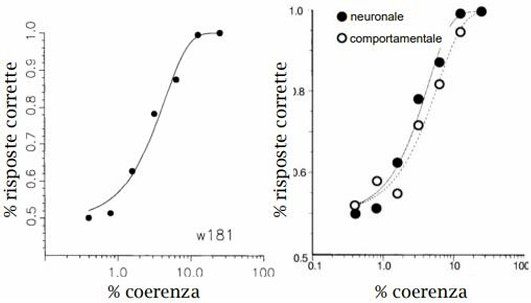
\includegraphics[width=0.80\textwidth]{images/image178.jpeg}
\end{figure}

L'AUC rappresenta la percentuale di corretti riconoscimenti da parte del neurone al variare della coerenza dello stimolo.
La capacità del classificatore di decodificare la risposta neuronale è quindi proporzionale alla capacità del soggetto di eseguire il compito percettivo, suggerendo che anche un singolo neurone può contenere informazioni sufficienti a spiegare il comportamento osservato.

\subsubsection{Conclusioni}

Per questo tipo di neurone, un modello a soglia può riprodurre la stessa dipendenza dalle condizioni di stimolo (\% di coerenza) osservata nei dati reali. Tuttavia, si tratta di un modello matematico semplificato, che non tiene conto dei meccanismi fisiologici reali (sinapsi, potenziali d'azione, integrazione temporale).
Sono quindi necessari modelli più realistici che includano:

\begin{itemize}
  \item reti di neuroni,
  \item variabilità biologica,
  \item meccanismi decisionali a livello del sistema nervoso.
\end{itemize}

\section{Applicazioni dell'encoding e decoding neuronale}

Le conoscenze derivate dallo studio del decoding neurale trovano applicazione nelle \textbf{interfacce cervello-computer (BCI).}
In questo contesto:

\begin{itemize}
  \item Microelettrodi impiantati nel cervello registrano l'attività elettrica di più neuroni.
  \item I segnali vengono trasmessi a un computer e analizzati tramite modelli di decoding (reti neurali, modelli statistici).
  \item Il sistema ricostruisce l'intenzione di movimento del soggetto (es. direzione o posizione desiderata).
  \item L'informazione viene inviata a un arto robotico o protesi.
  \item Il soggetto riceve feedback visivo o tattile per perfezionare il controllo in tempo reale.
\end{itemize}

\clearpage

\chapter{Modelli di reti cerebrali}
\section{Reti di neuroni e applicazioni}

\subsection{Complessità di modelli di neurone}
L'analisi dei modelli mostra come sia possibile costruire reti di neuroni che tengano conto della complessità cerebrale. Combinando diversi modelli, si può ottenere una rete in grado di rappresentare alcune proprietà del funzionamento organizzato del cervello. Si passa da modelli più semplici, che pur essendo meno recenti mantengono la loro utilità, a modelli più complessi che considerano tutti i meccanismi di membrana.

\subsection{Reti di neuroni}
\begin{figure}[H]
  \centering
  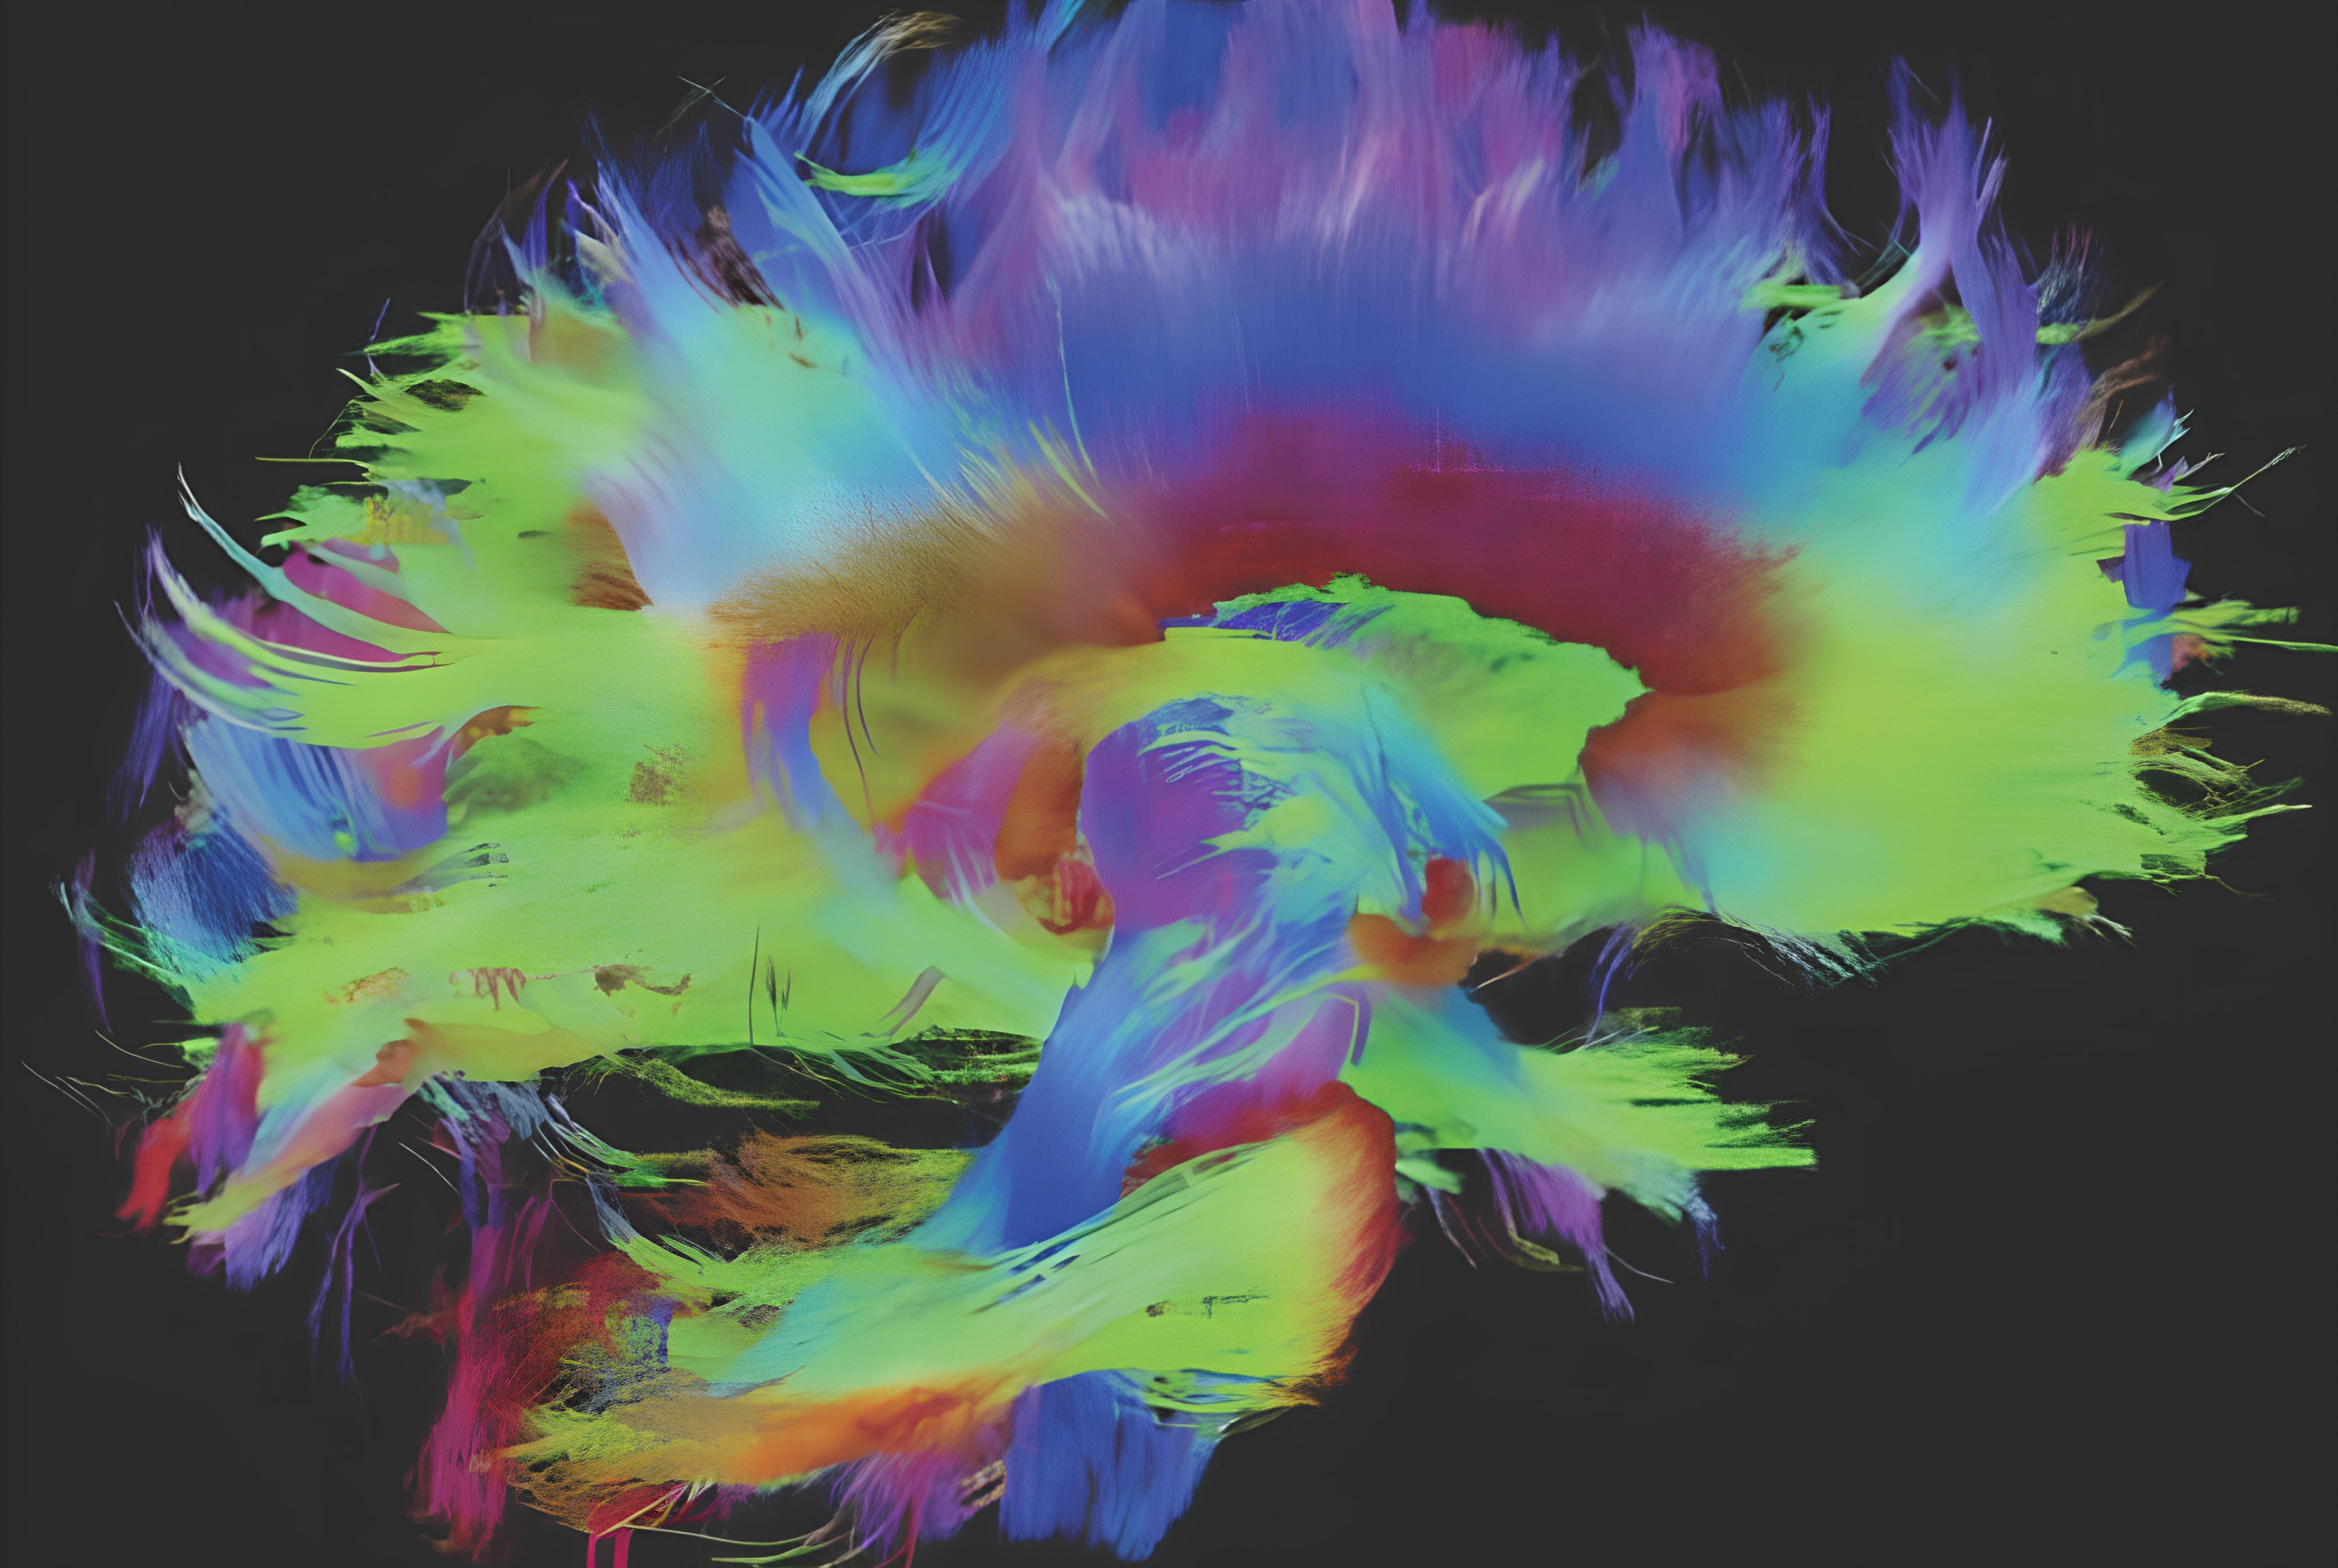
\includegraphics[width=0.80\textwidth]{images/image179(2).jpeg}
  \caption{Esempio di rete neuronale.}
  \label{fig:rete}
\end{figure}
Nel cervello umano, composto da circa 86 miliardi di neuroni, questi non lavorano isolatamente ma sono fittamente interconnessi, formando reti con numerosissimi punti di scambio di informazioni chiamati sinapsi (tra $10^{3}$ e $10^{5}$ per neurone). La complessità del cervello non dipende quindi dal numero dei neuroni, ma dalla quantità e dalla ricchezza delle loro connessioni, che consentono un'elaborazione delle informazioni estremamente complessa e performante, al punto da superare la nostra capacità di interpretarla.

\subsection{Connessioni cerebrali (fibre)}
La rete di neuroni può essere quantificata grazie a strumenti che analizzano le fibre nervose (assoni), spesso mielinizzate, che collegano i neuroni tra loro. Queste fibre non formano una rete disordinata, ma una struttura ordinata e simile tra diversi individui. I fasci di fibre, più o meno corposi, mettono in comunicazione varie aree del cervello e possono essere misurati con due tipi di metodi:
\begin{itemize}
  \item \textit{Metodi invasivi}, che prevedono la selezione del tessuto e il conteggio diretto delle fibre, danneggiando però il tessuto stesso;
  \item \textit{Metodi non invasivi}, che utilizzano immagini (spesso da risonanza magnetica) per ricostruire con precisione millimetrica il decorso delle fibre senza aprire la testa del paziente.
\end{itemize}
In questo modo è possibile ottenere la struttura della rete neuronale sia con strumenti invasivi che non invasivi.

\begin{figure}[H]
  \centering
  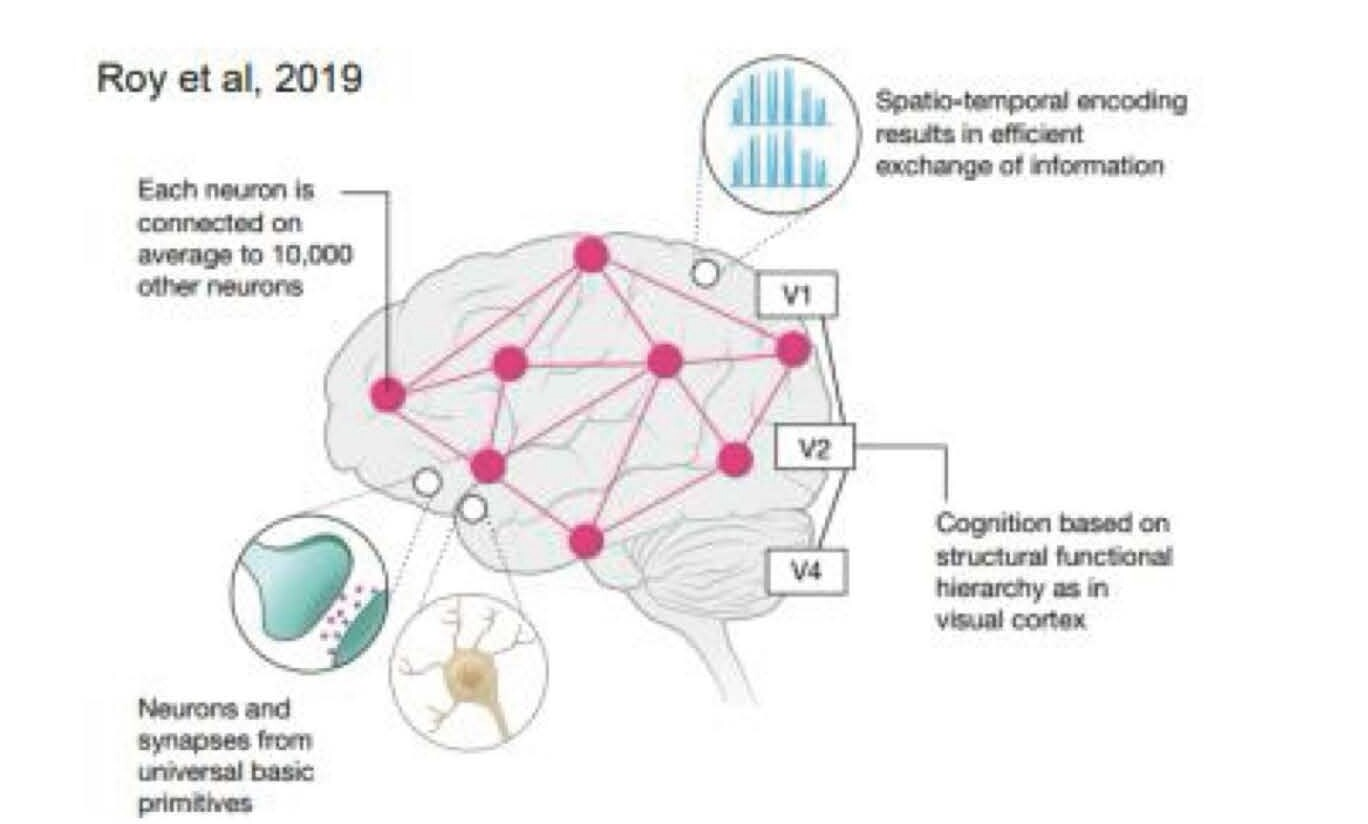
\includegraphics[width=0.80\textwidth]{images/image179(1).jpeg}
  \caption{Esempio di rete neuronale.}
\end{figure}


\textbf{Interazioni tra neuroni}
La rete di fibre forma circuiti di neuroni, in cui ogni neurone è un elemento collegato agli altri tramite interconnessioni fisiche. In media, con due sinapsi si raggiunge un altro neurone, ma possono esserci anche connessioni dirette o più lunghe, rendendo la rete molto fitta. Modellizzare il cervello come una rete è un problema complesso, poiché occorre capire come costruire una rete a partire dai modelli già studiati.

\textbf{Modelli elettrici (spiking models)}
I modelli che spiegano la generazione del potenziale d'azione, come quello di \textbf{Hodgkin-Huxley (H-H)}, rappresentano il modello di membrana più completo. Se si applicasse tale modello a ogni neurone (includendo tutti i rami sinaptici), si otterrebbe una rappresentazione molto complessa, utilizzabile solo per circuiti di piccole dimensioni.

Poiché è noto che il potenziale d'azione si genera al raggiungimento della soglia di apertura dei canali del sodio, non è necessario descrivere ogni volta il meccanismo: per questo si usa il modello \textbf{integra e spara}, che si concentra sul momento in cui si raggiunge la soglia e su come il potenziale influenza le cellule della rete.

Serve quindi un modello semplice che integri le conduttanze sinaptiche. Quando si vogliono analizzare alterazioni della generazione del potenziale d'azione, si usano modelli derivati e semplificati del modello di H-H, come quello di \textbf{Izhikevich}, che mostra cosa cambia in presenza di variazioni fisiologiche.

Questi modelli rappresentano in modo deterministico il comportamento della membrana nel tempo e vengono collegati in rete per simulare reti neuronali reali. Permettono di riprodurre il comportamento neuronale con precisione: sulla scala dei millisecondi per i potenziali d'azione e delle decine di millisecondi per i potenziali graduati. Tuttavia, richiedono molti parametri da stimare e grandi risorse di calcolo, oltre a segnali reali molto lunghi.

Registrazioni prolungate sono difficili da ottenere, perché il soggetto deve rimanere fermo a lungo e intervengono stanchezza, calo di attenzione e apprendimento. Anche mantenendo costanti stimoli e condizioni ambientali, nel tempo si verificano variazioni incontrollabili che introducono un aspetto stocastico, impedendo di considerare identiche le ripetizioni di uno stesso esperimento.

\textit{Limiti principali:}
\begin{itemize}
  \item Scala temporale molto dettagliata (da ms a centinaia di ms);
  \item Numerosi parametri da stimare;
  \item Elevata difficoltà computazionale;
  \item Mancata considerazione della stocasticità del comportamento neuronale;
  \item Difficoltà nel mediare su molti trial.
\end{itemize}

\textbf{Modelli encoding-decoding (firing models)}
Si tratta di modelli più semplici e computazionalmente leggeri, quindi più diffusi rispetto ai precedenti. Sono modelli a scatola nera, in cui non si fanno assunzioni ma si mette in relazione l'uscita del neurone con il suo ingresso. Ci si concentra su alcuni aspetti trascurandone altri: fenomeni come stanchezza o calo dell'attenzione vengono inclusi nella parte aleatoria del modello, rinunciando a descrivere ciò che non è rappresentabile e introducendolo nella componente probabilistica.

\textit{Vantaggi:}
\begin{itemize}
  \item Semplicità e leggerezza computazionale, grazie a una funzione che descrive il rapporto ingresso--uscita e quindi il comportamento del neurone;
  \item Scala temporale più contenuta, con meno trial e minori effetti di stanchezza;
  \item Introduzione della stocasticità, che permette a un singolo modello di rappresentare una famiglia di neuroni (reti più semplici);
  \item Possibilità di mediare le uscite su molti trial, ottenendo un comportamento più stabile; servono meno trial, quindi meno parametri e meno dati.
\end{itemize}

\textit{Limiti:}
\begin{itemize}
  \item Non considerano il sincronismo e funzionano bene solo con input scorrelati;
  \item Hanno minor accuratezza rispetto ai modelli di membrana: questi ultimi ricostruiscono la sequenza esatta dei potenziali d'azione, mentre i modelli semplici restituiscono solo la sequenza con la stessa frequenza di scarica, ma non identica;
  \item Si basano sulla curva di Tuning per simulare il comportamento del neurone, riproducendo spike con la stessa frequenza di scarica. Simulano quindi il neurone dal punto di vista del firing rate, perdendo risoluzione temporale ma compensandola con informazioni probabilistiche;
  \item Non descrivono i meccanismi fisiologici alla base della risposta neuronale, quindi non spiegano perché si generi un determinato potenziale d'azione.
\end{itemize}

\begin{figure}[H]
  \centering
  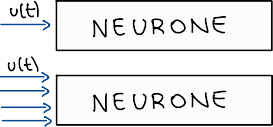
\includegraphics[width=0.80\textwidth]{images/image180.png}
  \caption{Confronto tra modello spiking e firing model.}
  \label{fig:confronto}
\end{figure}

In conclusione, non esiste un modello migliore: gli spiking models sono più dettagliati, precisi e spiegano i meccanismi fisiologici, ma sono più onerosi; i firing models sono più semplici e leggeri, ma con minore risoluzione e capacità esplicativa. I modelli basati su firing rate si avvicinano maggiormente alle reti di dimensioni paragonabili a quelle cerebrali reali. Il modello, pur definito per il singolo neurone, può essere applicato direttamente allo spiking system quando molti neuroni svolgono la stessa funzione, evitando di applicarlo a ciascuno singolarmente e semplificando così notevolmente la struttura complessiva.
\section{Applicazioni dei modelli computazionali dei sistemi neurali}

\textbf{Biomimetic Spiking Neural Network}

Si tratta di \textbf{reti neurali basate su modelli biomimetici spiking}: ``spiking'' indica l'uso di modelli elettrici realistici, mentre ``biomimetici'' significa che le reti imitano la biologia. Sono strumenti di \textbf{computazione artificiale}, realizzati tramite circuiti integrati programmabili (FPGA), che emulano circuiti neuronali reali per sfruttarne le capacità di calcolo.

Queste reti simulano \textbf{neuroni, sinapsi, membrana e plasticità}, corrispondenti alle sinapsi chimiche che permettono memoria e adattamento della risposta allo stimolo. La \textbf{plasticità }migliora le prestazioni del sistema, selezionando alcune funzioni e trascurandone altre.

L'approccio si basa sul \textbf{modello integra e spara}, versioni semplificate di Hodgkin-Huxley o modelli combinati come quello di Izhikevich. La rete viene poi implementata fisicamente in un circuito che replica \textbf{membrana, sinapsi, generazione del potenziale e plasticità}, modificandosi in base agli input.

Questo campo tecnologico potrebbe sostituire regioni cerebrali danneggiate, riproducendo dati fisiologici e fornendo stimoli corretti per ripristinare la funzione desiderata.

\textbf{Neuro-prostetica}

Le \textbf{neuro-protesi }sostituiscono o supportano funzioni compromesse (motorie, cognitive, sensoriali) a seguito di traumi o patologie.

Esempi:

\begin{itemize}
  \item \textbf{Protesi sensoriali in ingresso}: catturano segnali fisici (es. immagini) e li trasmettono al cervello, sostituendo percorsi naturali danneggiati.
  \item \textbf{Protesi motorie o ortesiche in uscita}: ripristinano la funzione muscolare; se l'arto esiste ma i muscoli non ricevono segnali, dispositivi esterni (esoscheletri) permettono la contrazione quando lo stimolo elettrico arriva.
\end{itemize}
I dispositivi possono \textbf{interfacciarsi direttamente con nervi o cervello}, sfruttando:

\begin{itemize}
  \item \textbf{Decodifica dei segnali cerebrali }per trasformare le intenzioni in azioni (output). La precisione e la velocità della decodifica sono cruciali.
  \item \textbf{Misura dei segnali fisici }per generare percezioni (input).
\end{itemize}
La precisione e la velocità della decodifica sono fondamentali. Questi sistemi si basano sulla conoscenza di come i neuroni rispondono a determinati input e permettono di stimolare o sostituire la funzione cerebrale, riproducendo i pattern fisiologici necessari. Ad oggi, non esiste nessuna protesi completamente efficiente nel replicare la funzione naturale.

\textbf{Neuroprotesi sensoriali}

\begin{itemize}
  \item \textbf{Uditive}: la più comune è l'impianto \textit{cocleare}, usato per restituire la funzione uditiva. Comprende un ricevitore, in grado di cogliere i segnali fisici che normalmente verrebbero colti, per poi convertirli in impulsi elettrici che stimolano il nervo acustico.
\end{itemize}
\begin{figure}[H]
  \centering
  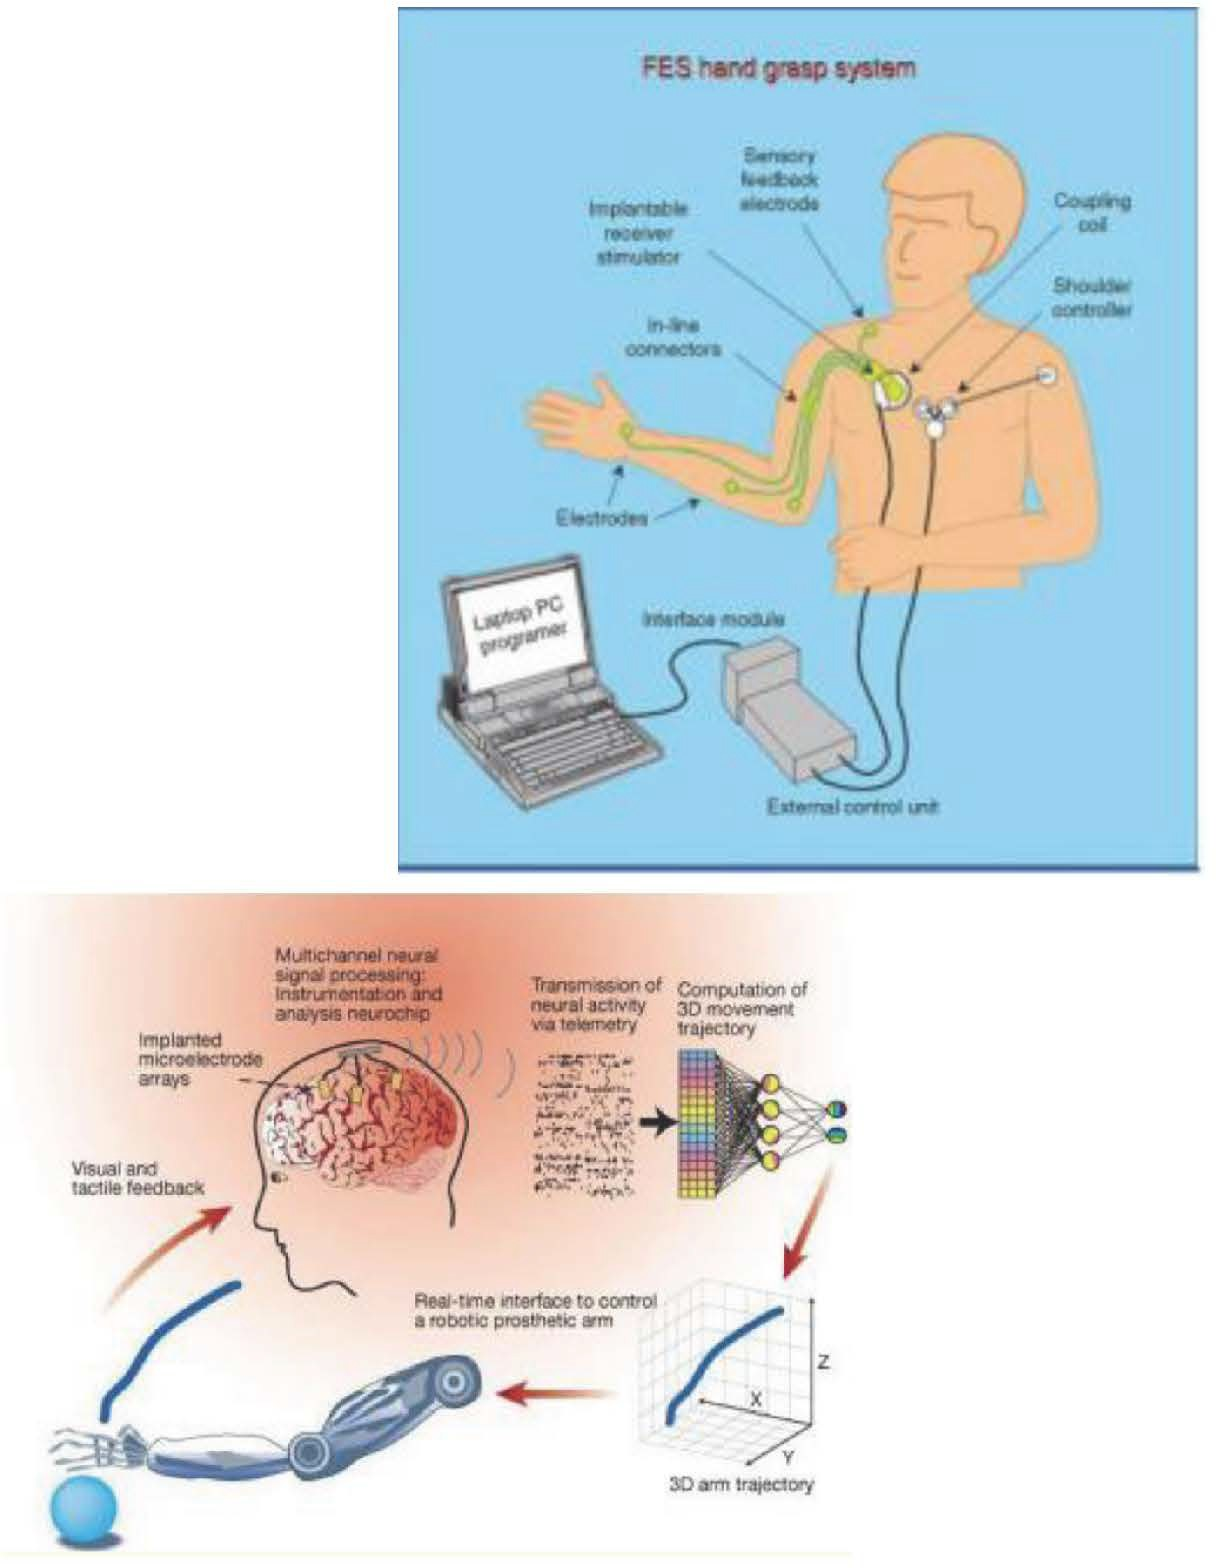
\includegraphics[width=0.80\textwidth]{images/image183.jpeg}
\end{figure}

Visive: attraverso una stimolazione della retina o della corteccia visiva, sono in grado di restituire la funzione visiva in caso di maculopatie o altre patologie. Per stimolare la corteccia, è necessaria una matrice di elettrodi che vadano a stimolare le famiglie neuronali.

\textbf{Neuroprotesi motorie}

Esistono \textit{arti robotici }dotati di tecnologie capaci di garantire movimenti precisi, accurati e rapidi, ma ancora poco efficaci nell'interfacciarsi direttamente con il cervello, mentre funzionano meglio se collegati ai muscoli. Da un lato vi è \textit{l'arto artificiale }che sostituisce quello mancante, dall'altro un sistema di \textit{stimolazione elettrica (FES) }applicato sulla cute per indurre la contrazione muscolare. Poiché la cellula muscolare è eccitabile,

la sua attività si basa sulla variazione del potenziale di membrana che genera un potenziale d'azione.

La stimolazione indiretta ha un ruolo importante nella neuro-riabilitazione, poiché permette di indurre la contrazione muscolare anche quando le connessioni tra

corteccia motoria e muscolo sono interrotte, come nelle lesioni spinali, dove il segnale inviato dalla corteccia non raggiunge il muscolo. In questi casi si misura l'attività corticale, si decodifica la volontà del soggetto e, bypassando le vie nervose danneggiate, si utilizza il segnale per controllare la stimolazione elettrica dei muscoli.

Quando l'arto è assente, il segnale decodificato viene inviato a un arto robotico che riproduce il movimento desiderato. In entrambi i casi è necessario un processo di \textit{decoding cerebrale}, realizzato mediante classificatori.

\textbf{Cervello artificiale}

Ad oggi, è in atto il progetto '\textit{The Human Brain Project}', il quale si basa su capacità e conoscenze modellistiche avanzate, così come le capacità di calcolo, conoscenze anatomiche e fisiologiche, in modo da ricostruire in maniera precisa i distretti e le aree del cervello.

\textbf{Reti neurali artificiali}

Le reti neurali artificiali sono una branca dell'informatica che mira a creare sistemi con altissime capacità di calcolo, in grado di elaborare grandi quantità di dati in tempi molto rapidi.

Alcuni sviluppatori di intelligenza artificiale hanno studiato la biologia del neurone per trarre ispirazione dalle reti naturali e progettare reti artificiali sempre più sofisticate. L'obiettivo non è sostituire le reti naturali, ma piuttosto integrarle e potenziarle.

\textbf{Modelli quantitativi in neuroscienze (conclusioni)}

I modelli quantitativi non si limitano a imitare la natura, ma aiutano a comprenderla: grazie, ad esempio, al modello di Hodgkin e Huxley si è potuto spiegare il funzionamento della membrana neuronale. Essi costringono inoltre a riformulare e formalizzare ipotesi sui fenomeni neurali. Possono integrare e riassumere osservazioni provenienti da esperimenti diversi, condotti con differenti risoluzioni e in vari laboratori, riunendo tutti i dati in un unico modello. Un buon modello permette anche di fare predizioni sperimentali: non solo riproduce le condizioni reali, ma consente di capire cosa accadrebbe in situazioni diverse, come mostrato dallo stesso modello di Hodgkin e Huxley sui canali ionici. Implementato in simulazioni, un modello quantitativo può contribuire alla creazione di dispositivi bio-ispirati, come robot, interfacce cervello-computer e reti neurali artificiali. Inoltre, un modello può rivelare la mancanza di dati, mettere in luce aspetti critici e suggerire esperimenti mirati, diventando così uno strumento utile per comprendere i limiti della ricerca e la direzione in cui progredire.

\end{document}